\documentclass[conference]{IEEEtran}
\IEEEoverridecommandlockouts
\usepackage{cite}
\usepackage{amsmath,amssymb,amsfonts}
\usepackage{algorithmic}
\usepackage{graphicx}
% All figures live in one directory alongside this file.
\graphicspath{{figures/}}
\usepackage{textcomp}
\usepackage{xcolor}
\usepackage{booktabs}
\usepackage{multirow}
\usepackage{array}
\newcolumntype{L}[1]{>{\raggedright\arraybackslash}p{#1}}
\usepackage{url}
\usepackage{placeins}
\usepackage{stfloats}

\makeatletter
\newcommand{\linebreakand}{%
  \end{@IEEEauthorhalign}
  \hfill\mbox{}\par
  \mbox{}\hfill\begin{@IEEEauthorhalign}
}
\makeatother

\begin{document}

\title{Spatial Transfer and Seasonal Sensitivity of Texture-Aware Sentinel-1/2 Land Use/Land Cover Classification in Madhya Pradesh}

\author{
\IEEEauthorblockN{Abhinav Kumar}
\IEEEauthorblockA{\textit{Department of Computer} \\
\textit{Science \& Engineering} \\
\textit{PDPM IIITDM} \\
Jabalpur, India \\
24bcs007@iiitdmj.ac.in}
\and
\IEEEauthorblockN{Aaditya Poddar}
\IEEEauthorblockA{\textit{Department of Computer} \\
\textit{Science \& Engineering} \\
\textit{PDPM IIITDM} \\
Jabalpur, India \\
24bcs002@iiitdmj.ac.in}
\and
\IEEEauthorblockN{Siddharth Ilayaraja}
\IEEEauthorblockA{\textit{Department of Computer} \\
\textit{Science \& Engineering} \\
\textit{PDPM IIITDM} \\
Jabalpur, India \\
24bcs292@iiitdmj.ac.in}
\and
\IEEEauthorblockN{Shivam Dubey}
\IEEEauthorblockA{\textit{Department of Computer} \\
\textit{Science \& Engineering} \\
\textit{PDPM IIITDM} \\
Jabalpur, India \\
23pcse03@iiitdmj.ac.in}
\linebreakand
\IEEEauthorblockN{Ashutosh Saxena}
\IEEEauthorblockA{\textit{Department of Computer} \\
\textit{Science \& Engineering} \\
\textit{PDPM IIITDM} \\
Jabalpur, India \\
24bcs041@iiitdmj.ac.in}
\and
\IEEEauthorblockN{Akshay Pandey}
\IEEEauthorblockA{\textit{Department of Computer} \\
\textit{Science \& Engineering} \\
\textit{PDPM IIITDM} \\
Jabalpur, India \\
drakshay@iiitdmj.ac.in}
\and
\IEEEauthorblockN{Aarav Jain}
\IEEEauthorblockA{\textit{Department of Computer} \\
\textit{Science \& Engineering} \\
\textit{PDPM IIITDM} \\
Jabalpur, India \\
24bcs004@iiitdmj.ac.in}
\and
\IEEEauthorblockN{Aniruddha}
\IEEEauthorblockA{\textit{Department of Computer} \\
\textit{Science \& Engineering} \\
\textit{PDPM IIITDM} \\
Jabalpur, India \\
aniruddha\_phd@iiitdmj.ac.in}
}

\maketitle

\begin{abstract}
Land use/land cover mapping over heterogeneous regions has to be assessed beyond the ground used for training. We evaluate five Google Earth Engine classifiers on Sentinel-2 reflectance and indices, optical texture, and Sentinel-1 backscatter and texture, for vegetation, water, built area, open land and agriculture in Madhya Pradesh. The 5,000 labelled points lie in four historical districts, which are excluded from every accuracy reported for the method; the remaining 44 are split by spatial block into 15 development districts, which carry every feature, model and hyperparameter choice, and 29 test districts scored once. Equal 59-day winter and summer windows of 2025 are compared. Feature composition matters more than feature count: two 19-band stacks of identical size differ by 4.91 points in summer on held-out ground. The selected Smile GTB pipeline agrees with a public-map consensus on 87.41\% of winter test samples (Kappa 0.843) and 73.85\% of summer samples (0.669), the summer figure falling to 71.71\% class-balanced because the consensus yields only 372 vegetation points against 580 of every other class. The winter ranking is not resolved: Holm-adjusted paired district tests give $p=0.125$ against SVM and Random Forest, and permuting the training rows alone moves the leading model by 0.38 points. Area-weighted over the domain the reference actually covers, 56.5\% of the test area and 95.86\% of it agriculture, agreement is 75.50\% $\pm$ 3.32, below the 95.86\% a constant agriculture predictor scores, so that estimator ranks maps by prevalence rather than by quality. At 1,350 locations sampled in both seasons under an unchanged reference label the seasonal fall is 8.67 points against 13.56 pooled, so the headline seasonal gap is partly a change of reference population. An independent product of comparable standing agrees with the consensus open-land label---the class the feature stack exists to separate---on only 28.1\% of the same winter points, so every figure here is conditional agreement over a stated domain and not verified accuracy.
\end{abstract}

\begin{IEEEkeywords}
Google Earth Engine, machine learning, Sentinel-1, Sentinel-2, LULC classification, Smile GTB, Madhya Pradesh.
\end{IEEEkeywords}

\section{Introduction}
Reliable land use/land cover (LULC) information underpins ecological monitoring, urban growth assessment, agricultural statistics and sustainable land management \cite{r1}, \cite{r3}. Ground surveys are slow, labour-intensive and limited in spatial coverage. Optical satellites such as Sentinel-2 and radar satellites such as Sentinel-1 now give free, repeated coverage of the same ground \cite{r4}, \cite{r6}. Machine learning can map those pixels to named classes \cite{r7}--\cite{r9}, and Google Earth Engine runs that work on large archives without moving the images to a local disk \cite{r10}.

Five classes are used throughout this paper: vegetation, water, built area, open land and agriculture. Water and vegetation are easy in optical data because water is dark in the near infrared and green plants are bright there \cite{r2}. Built area and open land are not. Taking the class median over the labelled points on the winter composite, we measured red reflectance of 0.222 for dry open ground against 0.226 for built surfaces, and short-wave infrared of 0.334 against 0.342, a separation smaller than the within-class spread of either. Colour alone cannot split those two materials. Texture (rough roofs versus smooth soil) and radar (double-bounce from walls) supply the missing evidence.

Accuracy also depends on how the map is checked. Labelled points sit in clusters, so a random train-test split often puts neighbouring 10\,m pixels on both sides and overstates skill \cite{r18}, \cite{r19}. Cultivated land is the largest land type in Madhya Pradesh and it is not spectrally stable: a field is green in winter and often bare earth in the pre-monsoon window, so agriculture and open land exchange members between seasons. This study therefore trains only on labels from Jabalpur and its immediate neighbourhood, scores every reported figure against a consensus of independent public products over 29 test districts that no model or feature choice was allowed to see, and reports both a winter and a summer window.

Random Forest, support vector machines and gradient boosting are the classifiers most often reported for Sentinel LULC \cite{r7}--\cite{r9}, \cite{r13}, and fusing optical with radar for regional land cover is established practice \cite{r33} rather than a contribution this paper claims. What such studies rarely isolate is the specific confusion that appears once vegetation and water are no longer the only classes: dry open land versus built area. Bright dry soil and concrete are near identical in Sentinel-2 reflectance, so a model that sees only per-pixel colour has little to work with. Texture is expected to help on the precision side, by refusing to call a smooth surface built, and radar on the recall side, since double-bounce from a wall-and-ground corner has no reflectance analogue. We test that expectation by controlled ablation on a held-out development population rather than by adding groups all at once, and we report what the ablation measures---predictive contribution---rather than treating it as a direct measurement of scattering physics.

The contribution is an explicitly partitioned, within-state transfer assessment of a texture-aware optical-radar LULC workflow. Development-only feature selection compares both feature count and feature identity, while held-out evaluation distinguishes pooled and class-balanced sample agreement from area-weighted agreement on the covered reference domain, and reports the trivial constant-class baseline that the last of these must be read against. The analysis also documents seasonal failure patterns and the dependence of conclusions on reference and validation design. It does not propose a new classifier and does not claim universal spatial generalisation.

Concretely, the paper contributes: (i) a GEE workflow that fuses Sentinel-2 reflectance, bareness and built-up indices, GLCM texture and Sentinel-1 radar for five land use/land cover classes; (ii) a controlled ablation that attributes the predictive gain of each feature family, and a feature-stack reduction chosen on development districts and re-tested on held-out ones, which shows that the identity of the retained bands, not their number, is what the reduction turns on; (iii) an evaluation over 44 historical districts of Madhya Pradesh against a public-map consensus whose per-class screening rules are stated explicitly and are not uniform across classes, partitioned by spatial block into disjoint development and test halves so that the 29 test districts carry every reported figure, with the consensus-covered fraction of that area reported alongside; (iv) a comparison of five machine-learning classifiers under that protocol in two seasons, with multiplicity-adjusted paired inference; (v) a quantified account of how much the reported accuracy depends on the validation protocol and on the class composition of the held-out fold rather than on the classifier, measured over eight contiguous block realisations with matched training budgets; (vi) four audits of the assessment itself---the grid the texture bands were actually computed on, the fitting variability the sampling intervals do not describe, the seasonal fall measured at fixed reference locations, and the class-specific disagreement between the consensus and an independent product---each of which changes how a headline figure may be read; and (vii) a served map interface that applies the same models to any drawn polygon, whose delivered raster is assessed separately from the raw classification the accuracies describe.

Every table, figure and quoted number in this paper is generated from one frozen result archive of flat files, listed in the Data and Code Availability section, and the arithmetic identities relating each confusion matrix to the metrics printed from it are asserted rather than assumed.

\section{Literature Review}
The field of Land Use and Land Cover (LULC) classification has undergone significant transformations, moving from traditional local-scale mapping using single-sensor data to planetary-scale monitoring using multi-sensor fusion and advanced machine learning in cloud environments. This section systematically reviews the literature, categorised into the evolution of cloud computing platforms, the use of optical and SAR data, the integration of spatial texture, machine learning applications, and the specific challenge of differentiating built-up surfaces from bare land; Table~\ref{tab_lit} summarises the studies closest to the present design.

\subsection{Cloud-Based Remote Sensing and Google Earth Engine}
Traditional remote sensing workflows required the downloading, storage, and local processing of large satellite imagery datasets, a bottleneck that severely limited large-scale and multi-temporal studies. The introduction of cloud computing platforms, notably Google Earth Engine (GEE) \cite{r10}, revolutionized this paradigm. GEE provides a massive, multi-petabyte catalog of satellite imagery and geospatial datasets, coupled with planetary-scale analysis capabilities. Researchers can now execute complex classification algorithms across thousands of scenes without the need for local data management. 
Numerous studies have demonstrated GEE's capability in regional and global LULC mapping. For instance, Zhao et al. \cite{r3} compared multiple machine learning algorithms within GEE for LULC classification, highlighting its efficiency in handling large-scale features. Similarly, the development of global products like Dynamic World \cite{r15} and ESA WorldCover \cite{r14} rely heavily on cloud infrastructure to process near real-time data. GEE's ability to quickly generate cloud-free composites by applying pixel-level masking (e.g., QA60 for Sentinel-2) over time series data has become a standard practice in modern remote sensing workflows.

\subsection{Optical Imagery in Land Cover Classification}
Optical remote sensing, primarily from the Landsat and Sentinel-2 programs, has been the foundational data source for land cover mapping. Sentinel-2 \cite{r4}, \cite{r5}, with its 10-meter and 20-meter spatial resolutions and 5-day revisit time, has enabled highly detailed and timely mapping of the Earth's surface. 
Optical data is particularly effective for mapping vegetation and water bodies due to distinct spectral signatures. The visible and near-infrared (NIR) bands are commonly used to compute indices that enhance these features. The Normalised Difference Vegetation Index (NDVI) \cite{r1}, \cite{r2} exploits the high reflectance of healthy vegetation in the NIR band and its strong absorption in the red band. The Soil-Adjusted Vegetation Index (SAVI) \cite{r24} improves upon NDVI in areas with sparse vegetation by minimizing soil background influences. For water bodies, the Normalised Difference Water Index (NDWI) \cite{r22} leverages the absorption of NIR by water to distinguish it from terrestrial features.
However, optical imagery alone faces significant challenges in complex landscapes. Cloud cover and shadows can severely limit data availability in certain regions and seasons, necessitating the use of multi-temporal composites. Furthermore, while optical indices are highly effective for vegetation and water, they often struggle with non-vegetated terrestrial surfaces, leading to spectral confusion.

\subsection{Synthetic Aperture Radar (SAR) and Sensor Fusion}
To overcome the limitations of optical sensors, Synthetic Aperture Radar (SAR), particularly from the Sentinel-1 mission \cite{r6}, is increasingly being integrated into LULC workflows. SAR operates in the microwave spectrum, allowing it to penetrate clouds and provide consistent data regardless of weather or solar illumination.
More importantly, SAR provides information about the physical structure and dielectric properties of the target surface, which is complementary to the chemical and physiological information provided by optical sensors. Sentinel-1 C-band SAR data typically includes co-polarized (VV) and cross-polarized (VH) backscatter. VV backscatter is highly sensitive to surface roughness and the double-bounce scattering mechanism characteristic of vertical structures in urban areas. VH backscatter is sensitive to volume scattering, making it useful for differentiating vegetation types.
The fusion of Sentinel-1 and Sentinel-2 data has been shown to yield higher classification accuracies than using either sensor independently \cite{r3}, \cite{r14}, \cite{r16}. By combining the spectral detail of Sentinel-2 with the structural and textural information of Sentinel-1, classifiers can better distinguish between classes that have similar spectral profiles but different physical structures, such as forests versus agricultural fields, or urban areas versus bare soil.

\subsection{The Role of Textural Features in Classification}
While pixel-based classification relies solely on the spectral value of individual pixels, texture analysis incorporates the spatial context by examining the relationships between a pixel and its neighbours. The Grey-Level Co-occurrence Matrix (GLCM) \cite{r20} is the most widely used method for extracting texture features in remote sensing.
GLCM calculates how often pairs of pixels with specific values and in a specified spatial relationship occur in an image, generating metrics such as contrast, variance, entropy, and homogeneity. In LULC classification, texture is particularly valuable for mapping heterogeneous classes like urban areas. Urban landscapes are characterized by a high spatial frequency of different materials (roofs, roads, shadows, vegetation), resulting in high GLCM contrast and variance. In contrast, surfaces like water or bare soil tend to be spatially homogeneous, resulting in lower contrast and higher homogeneity.
Adding optical GLCM texture, usually computed on the NIR band, has been shown to improve the separation of built-up areas from other non-vegetated surfaces \cite{r8}, \cite{r20}. Similarly, radar texture computed on Sentinel-1 VV backscatter further enhances the detection of urban fabric by capturing the local spatial variation of radar returns.

\subsection{Machine Learning Algorithms for Remote Sensing}
The application of machine learning has significantly improved the accuracy and automation of LULC classification compared to traditional maximum likelihood or rule-based methods. Several algorithms have become standard in the field \cite{r8}:
\begin{itemize}
    \item \textbf{Random Forest (RF):} An ensemble of decision trees whose output is the modal class \cite{r9}, \cite{r11}. Its popularity in remote sensing rests on robustness to outliers and to high-dimensional feature spaces, and on being comparatively forgiving of its settings, a property Section~\ref{sec:tuning} finds does not hold here.
    \item \textbf{Support Vector Machines (SVM):} SVM finds the maximum-margin separating hyperplane in a high-dimensional feature space \cite{r7}, \cite{r12}, and with a Radial Basis Function kernel can model non-linear class boundaries. It is computationally demanding on large training sets and, being distance-based, is sensitive to the relative scaling of its inputs.
    \item \textbf{Gradient tree boosting:} boosting \cite{r27} builds trees sequentially, each new tree fitting the residual error of the ensemble so far. It often outperforms RF on LULC tasks provided its learning rate, depth and tree count are tuned. Implementations differ more than the shared name suggests, and the distinction matters for reproducibility: this study uses the Smile library's gradient tree boosting as exposed by Earth Engine, which is not the XGBoost of Chen and Guestrin \cite{r13} and offers neither its regularised objective nor its sparsity-aware split finding.
    \item \textbf{k-Nearest Neighbours (KNN) and CART:} KNN classifies a pixel by majority vote among its $k$ nearest training samples, and Classification and Regression Trees construct a single decision tree. Both are usual baselines and generally trail ensemble methods in complex landscapes. KNN's dependence on a distance metric also makes it, with SVM, the classifier most exposed to unscaled features, a point Section~\ref{sec:models} returns to.
\end{itemize}

\subsection{Deep Learning versus Traditional Machine Learning}
In recent years, deep learning (DL), particularly Convolutional Neural Networks (CNNs), has gained immense popularity in remote sensing due to its ability to automatically extract hierarchical spatial features from imagery. Architectures such as U-Net, ResNet, and Fully Convolutional Networks (FCNs) have been successfully applied to semantic segmentation tasks, often outperforming traditional machine learning algorithms in terms of pixel-level accuracy \cite{r15}. 
However, traditional machine learning algorithms like Random Forest and Smile GTB remain highly relevant and widely used, especially within platforms like Google Earth Engine. DL models typically require massive amounts of labelled training data, extensive computational resources (GPUs), and complex hyperparameter tuning. Furthermore, DL models often act as ``black boxes,'' making it difficult to interpret feature importance, a critical requirement in many environmental studies where understanding the physical drivers of classification is as important as the classification itself.
In contrast, tree-based models permit a controlled ablation in which one feature family is added or removed and the change in a named error is read off directly. Given the constraints of server-side execution limits in GEE for custom architectures and that ablation requirement, this study uses traditional machine learning algorithms throughout. No deep-learning baseline was trained here, so nothing in this paper compares the two families: statements about their relative accuracy would need a CNN scored on the same reference, the same districts and the same split, and that experiment was not run.

\subsection{Feature Selection and Dimensionality Reduction}
The proliferation of satellite sensors has led to a dramatic increase in the dimensionality of remote sensing datasets. While adding more features (spectral bands, indices, texture metrics, multi-temporal composites) can provide more information, it also increases the risk of the ``Hughes phenomenon'' \cite{r32} or the curse of dimensionality. High-dimensional feature spaces can lead to model overfitting, increased computational complexity, and reduced classification accuracy if the training sample size is not proportionally large.
To address this, researchers employ feature selection and dimensionality reduction techniques. Principal Component Analysis (PCA) is commonly used to transform correlated spectral bands into uncorrelated components. Alternatively, feature importance metrics derived from Random Forest or gradient boosting models can be used to identify and retain only the most discriminative features.
Effective feature selection is particularly crucial in GEE workflows, where computational limits can cause memory exhaustion during the training of complex models over large areas. Identifying a lean, optimised feature stack not only accelerates the classification process but also enhances model generalization. This study incorporates a feature ablation methodology to identify a compact subset of features. Its result is a qualified one: a 19-band stack outperforms the full 27-band stack only when the 19 are selected on data held apart from the data they are scored on, and a differently chosen stack of the same size is markedly worse. Band count is therefore a poor proxy for the quality of a reduction.

\subsection{Spatial Autocorrelation and Accuracy Assessment Protocols}
A critical, yet often overlooked, aspect of remote sensing literature is the methodology used for accuracy assessment. Traditional random train-test splits assume that samples are independent and identically distributed. However, geospatial data exhibits strong spatial autocorrelation, governed by Tobler's First Law of Geography \cite{r31}: near things are more related than distant things.
When labelled pixels are sampled from clustered polygons, a random split often places spatially adjacent pixels into both the training and testing sets. Because adjacent pixels share nearly identical spectral and environmental characteristics, the model essentially ``memorizes'' the local spatial structure rather than learning generalizable class rules. This phenomenon leads to artificially inflated accuracy metrics, a problem highlighted by Roberts et al. \cite{r18} and Ploton et al. \cite{r19}.
To obtain a realistic estimate of model performance, rigorous spatial validation protocols are required. Techniques such as spatial block cross-validation or testing on entirely independent geographic regions provide a more honest assessment of a model's ability to generalize to unseen data. This study addresses this gap in the literature by employing a strict spatial generalization protocol: models are trained on labelled points from one district and its immediate neighbourhood, and every reported figure is measured against a high-confidence consensus of independent public maps over 29 districts that took no part in any modelling choice.

\subsection{The Challenge of Disambiguating Urban and Bare Land}
A persistent and significant challenge in remote sensing is the spectral confusion between built-up (urban) areas and bare, open land (or dry soil). Both classes typically lack vegetation cover and can exhibit high reflectance in the visible and short-wave infrared (SWIR) bands, while absorbing near-infrared (NIR) radiation.
Traditional indices designed to extract built-up areas, such as the Normalised Difference Built-up Index (NDBI) \cite{r21}, the Urban Index (UI), and the Index-based Built-up Index (IBI) \cite{r23}, frequently struggle to differentiate these two classes. For instance, dry riverbeds, fallow agricultural fields, and rocky outcrops often yield NDBI values similar to those of concrete and asphalt \cite{r26}.
Researchers have explored various techniques to resolve this confusion. One approach involves multi-temporal analysis, exploiting the temporal stability of urban structures compared to the seasonal variability of bare soil (which may become vegetated during wet seasons). Another approach relies on thermal infrared data to distinguish the thermal inertia of human-made materials from natural soil, although this is not possible with Sentinel-2.
The most promising approach, which forms the core of the present study, is the integration of physical and structural information. The double-bounce radar backscatter from Sentinel-1 is reported as a strong signature for vertical urban structures that flat bare soil does not reproduce. Simultaneously, the spatial roughness captured by GLCM texture metrics differentiates the complex physical arrangement of urban environments from the smooth surfaces of open land. This study contributes to the literature by quantifying the exact gain of these specific features through a controlled ablation study.

\subsection{Summary of State-of-the-Art LULC Products}
Recent years have seen the release of several global, high-resolution LULC maps generated using cloud computing and machine learning. ESA WorldCover \cite{r14} provides a 10m global land cover map based on Sentinel-1 and Sentinel-2 data, achieving high overall accuracy. Dynamic World \cite{r15} offers near real-time, 10m LULC probabilities by applying deep learning to Sentinel-2 imagery. Specialist products like WorldCereal \cite{r16} focus on specific classes, providing seasonal temporary-crop and active-cropland maps for the 2021 epoch. De Luca et al.\ \cite{r33} is the closest published design to the present one, applying an open-source Random Forest, with an exhaustive parameter search, to fused Sentinel-1 and Sentinel-2 data for regional land cover in a Mediterranean setting. It is a single-classifier study, so the multi-classifier comparison is a difference between that work and this one rather than a shared feature. The gap this paper addresses is not that sensor fusion is new but that regional studies of this shape rarely separate the population a choice was made on from the population it is reported on, and rarely state the domain a reference actually covers.
While these global products represent significant achievements, they often exhibit regional biases or reduced accuracy in transitional zones, such as the complex landscapes of Madhya Pradesh. Localized studies, tuned to specific regional characteristics and validated against robust independent protocols, remain essential for accurate environmental monitoring and planning. The present study utilises these state-of-the-art products not as competitors, but as a high-confidence consensus reference to validate the proposed regional models.

\begin{table*}[!t]
\caption{Summary of Key Literature in Cloud-Based Land Cover Classification}
\label{tab_lit}
\begin{center}
\renewcommand{\arraystretch}{1.3}
\begin{tabular}{p{2.5cm}p{2.5cm}p{3cm}p{3cm}p{5cm}}
\toprule
\textbf{Study} & \textbf{Sensors} & \textbf{Methodology} & \textbf{Study Area} & \textbf{Key Findings} \\
\midrule
Pal \& Mather \cite{r7} & Landsat ETM+ & SVM, Max Likelihood & Eastern England & SVM outperforms traditional classifiers but struggles with spectrally similar classes. \\
Gislason et al. \cite{r9} & Landsat MSS & Random Forest, CART & Colorado, USA & Random Forest provides higher accuracy and robustness to noise compared to single decision trees. \\
Gorelick et al. \cite{r10} & Multi-sensor & Google Earth Engine & Global & Introduced GEE, enabling planetary-scale fusion of optical and radar data for LULC. \\
Maxwell et al. \cite{r8} & Optical \& Radar & RF, SVM, KNN & Review Study & Emphasized the necessity of feature engineering (texture, indices) over simply choosing complex algorithms. \\
Zhao et al. \cite{r3} & Sentinel-1 \& 2 & RF, SVM, CART & Regional & Highlighted that multi-sensor fusion significantly improves accuracy over optical-only classifications. \\
Zha et al. \cite{r21} & Landsat TM & NDBI, NDVI & Nanjing, China & NDBI effectively extracts urban areas but shows significant confusion with bare land. \\
Xu \cite{r23} & Landsat ETM+ & IBI, NDBI & Fuzhou, China & IBI improves urban extraction by suppressing vegetation and water, but bare soil remains problematic. \\
Rasul et al. \cite{r26} & Landsat 8 & Multiple Indices & Erbil, Iraq & Comprehensive demonstration that optical indices fail to separate dry bare soil from built-up areas. \\
Zanaga et al. \cite{r14} & Sentinel-1 \& 2 & Gradient-boosted ensemble & Global & Global 10\,m map for the 2021 epoch utilising both optical and SAR data, with high global accuracy and known regional confusion. \\
Brown et al. \cite{r15} & Sentinel-2 & Deep Learning (FCN) & Global & Near real-time mapping; acknowledges confusion between built and bare classes in semi-arid environments. \\
Van Tricht et al. \cite{r16}& Sentinel-1 \& 2 & Machine Learning & Global & Temporary-crop and active-cropland products for 2021; used here only as the agriculture specialist, and only its annual \texttt{temporarycrops} layer, the seasonal active-cropland markers having returned no valid pixels over the study area. \\
De Luca et al. \cite{r33} & Sentinel-1 \& 2 & RF only & Mediterranean & Closest prior study in design: open-source classifiers on fused optical and SAR for regional land cover, and the comparison point for the workflow reported here. \\
\textbf{This Study} & \textbf{Sentinel-1 \& 2} & \textbf{Five GEE classifiers} & \textbf{Madhya Pradesh} & \textbf{Quantifies how much SAR and texture reduce built/open confusion, and separates class-balanced from area-weighted agreement on 29 districts held out before any selection.} \\
\bottomrule
\end{tabular}
\end{center}
\end{table*}

\section{Study Area and Data}

\subsection{Study area}
Training labels were collected in Jabalpur district, Madhya Pradesh, centred near $79.93^\circ\text{E}$, $23.18^\circ\text{N}$. The district mixes deciduous vegetation, the Narmada and smaller water bodies, the urban fabric of Jabalpur city, rocky open land, and cultivated fields, so all five classes occur in one place. The outline used throughout is the FAO GAUL 2015 level-2 polygon for Jabalpur, whose measured geodesic area is $4{,}021.3\text{ km}^2$; the same geometry drives the accuracy assessment and the interactive application, so a figure reported for ``Jabalpur'' always means this polygon. The labelled points were not confined to it: their bounding box spans $79.38^\circ$--$80.52^\circ\text{E}$ and $22.84^\circ$--$23.59^\circ\text{N}$, and 872 of them lie outside the polygon (Section~\ref{sec:labels}).

The evaluation region is the whole of Madhya Pradesh, located in the geographic heart of India, providing an exceptionally diverse testing ground for land cover classification models. Covering an area of approximately $308,252\text{ km}^2$, spanning roughly $74.0^\circ\text{E}$ to $82.8^\circ\text{E}$, the state was split into the 48 district polygons of FAO GAUL 2015 level~2, which is the boundary set used throughout this paper. That vintage predates the districts created between 2018 and 2023, so Madhya Pradesh now administers 55 districts against these 48 polygons. They are therefore described throughout as historical evaluation units rather than as the state's current districts. 

The climate is broadly characterized as subtropical, with a distinct monsoon season (June to September) that heavily influences the phenology of vegetation and the temporal dynamics of agriculture. The topography is highly varied. The Malwa plateau in the west is characterized by fertile black cotton soils that support intensive agriculture. The northern regions, including the Chambal valley, feature deep ravines and rugged terrain. The central and eastern parts of the state are dominated by the Vindhya and Satpura mountain ranges, which harbor dense deciduous forests and significant tribal populations. The southern regions transition into the Deccan plateau, characterized by varied geological formations and mixed land use.

This diversity means that a single land cover class carries a large intra-class spectral variance across the state. The ``agriculture'' class spans irrigated wheat in the Narmada valley, rainfed millet in the drylands and fallow fields waiting for the monsoon; ``open land'' spans the rocky outcrops of Bundelkhand, the dry riverbeds of the Chambal and barren soil on agricultural peripheries. None of these has a full counterpart in the Jabalpur training set, so scoring the models here measures spatial generalisation rather than interpolation.

\begin{figure*}[!t]
\centering
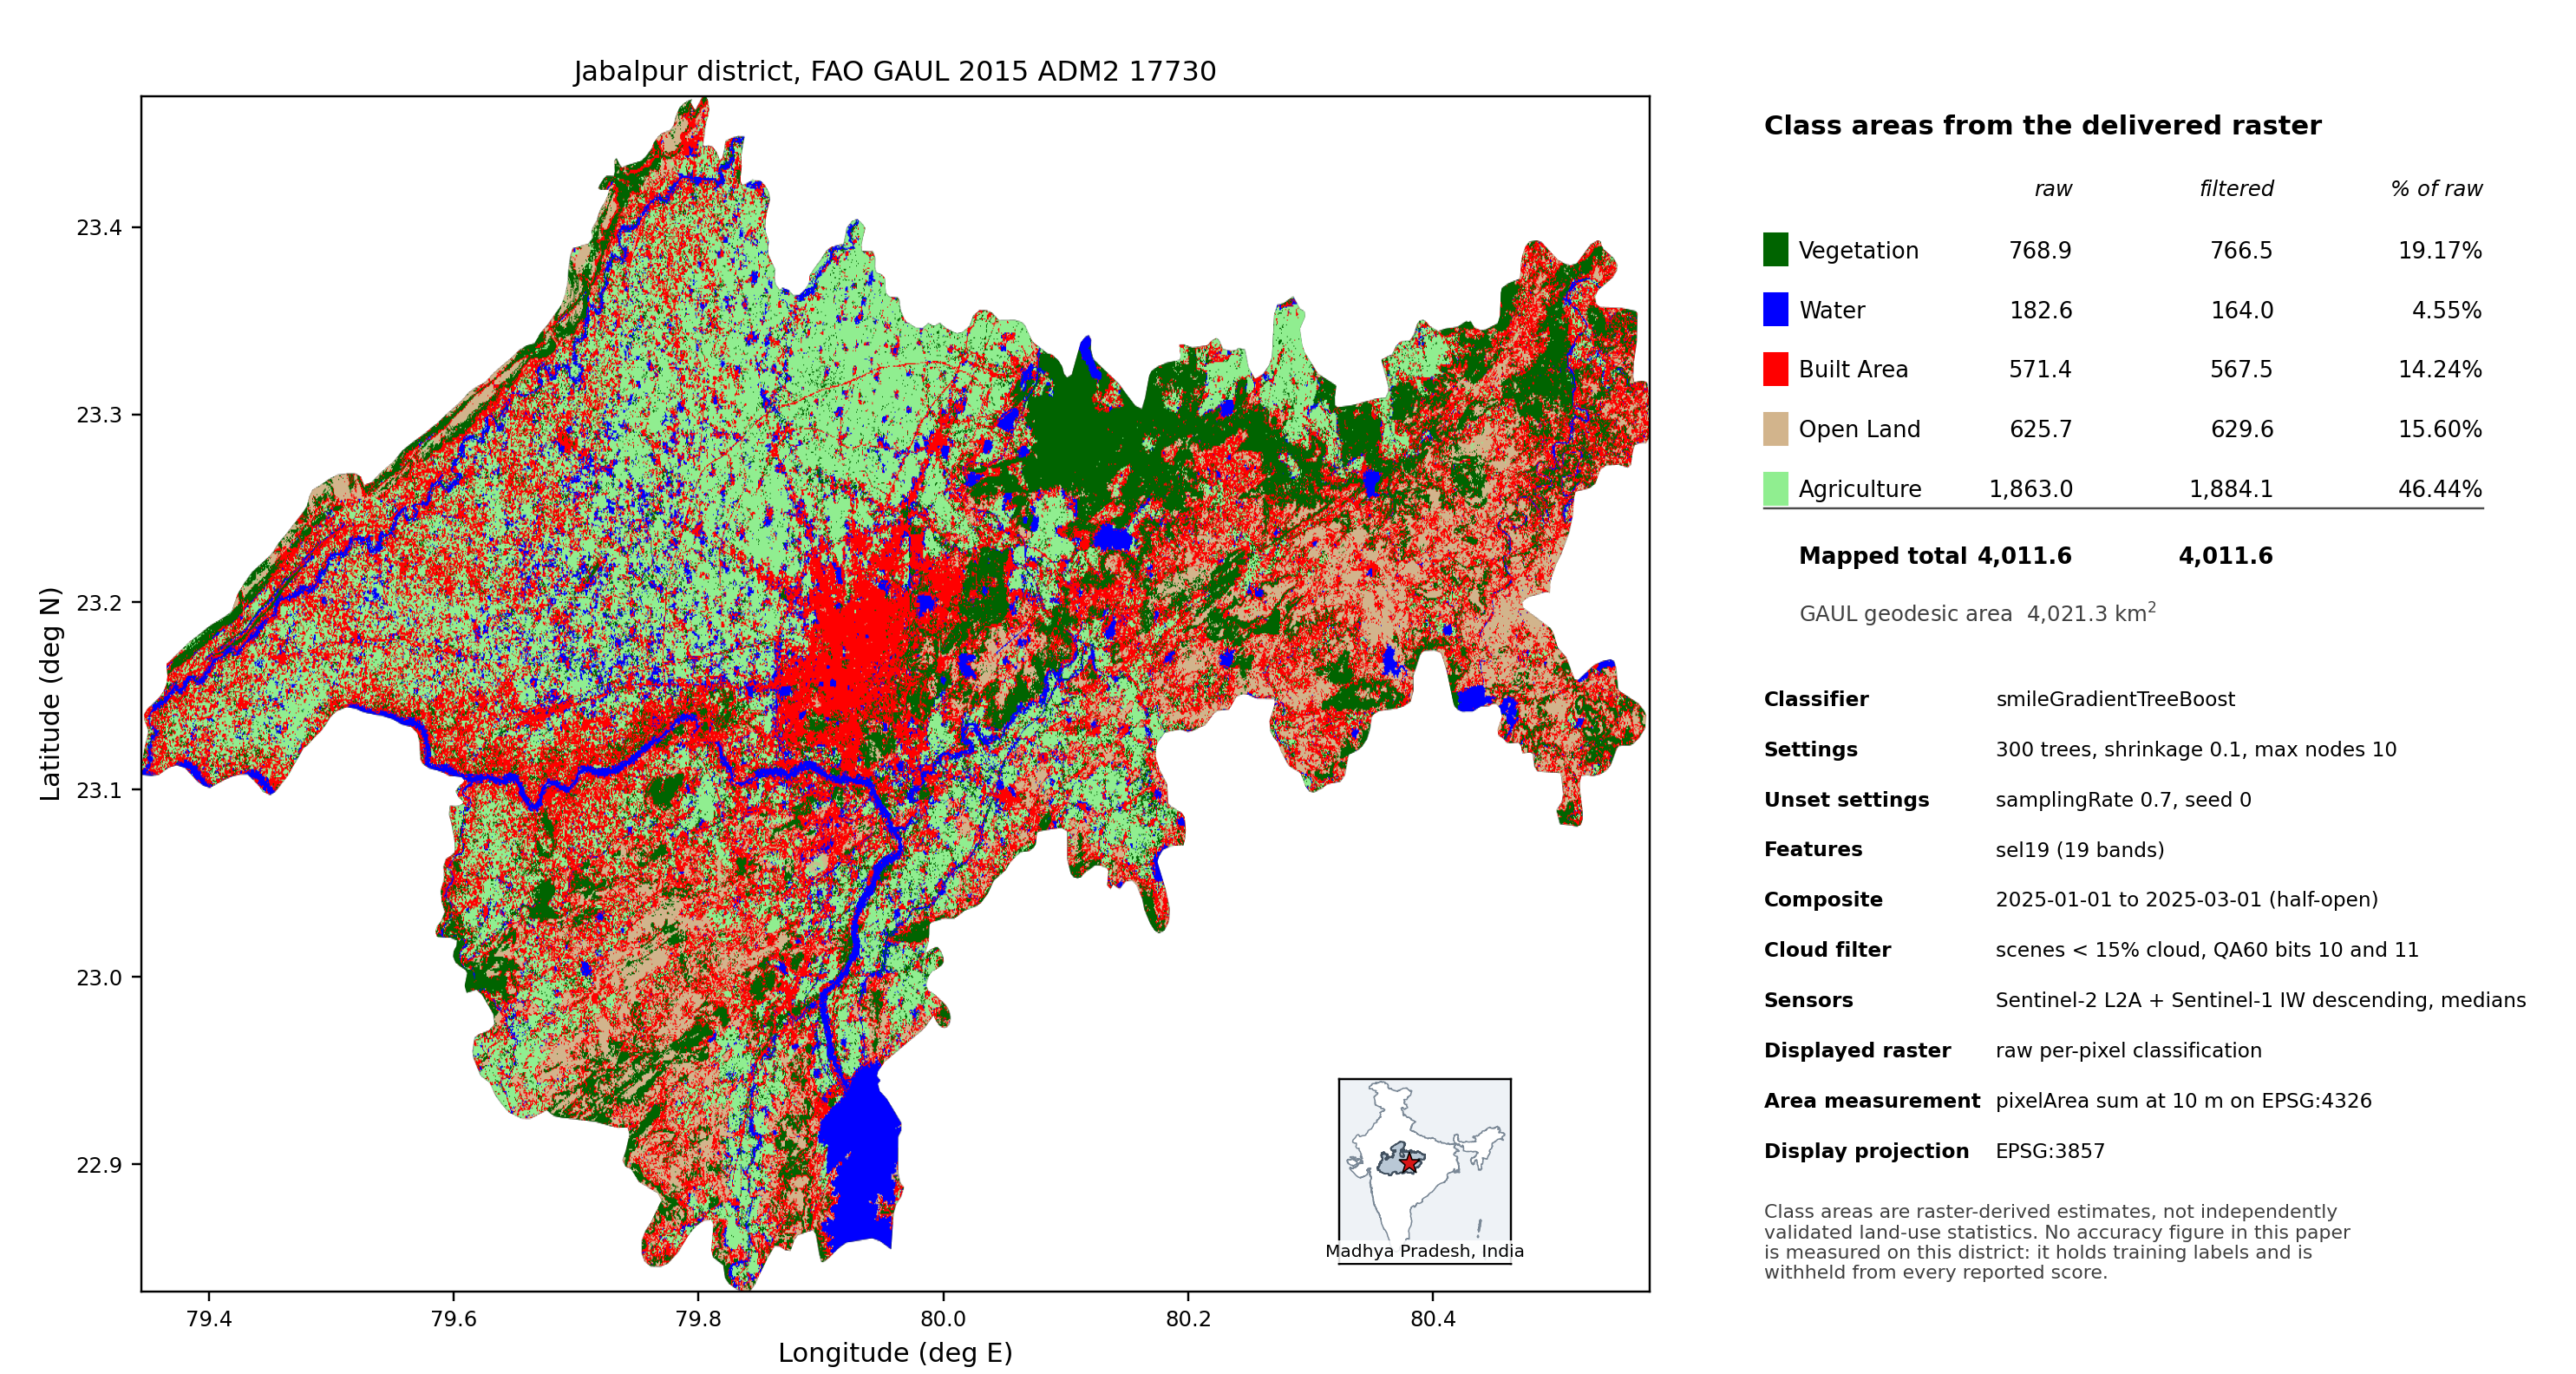
\includegraphics[width=0.95\textwidth]{fig1_jabalpur_map.png}
\caption{Five-class prediction for the FAO GAUL 2015 Jabalpur polygon (ADM2 17730) on a 10\,m grid, from the frozen Smile GTB model on the winter 2025 composite. The displayed raster is the raw per-pixel classification. Raw and majority-filtered class areas both total 4{,}011.65\,km$^2$ against the polygon's geodesic 4{,}021.33\,km$^2$; these are raster-derived estimates, not validated land-use statistics. The inset locates the state within India. Jabalpur is one of the four districts withheld from every reported accuracy (Fig.~\ref{fig:split_map}).}
\label{fig:jabalpur_map}
\end{figure*}

Fig.~\ref{fig:jabalpur_map} shows a 10\,m five-class map of the Jabalpur polygon, produced by the frozen classifier the dashboard serves. The urban core is mapped as built area, the Narmada as water, cultivated land as agriculture and the wooded ridges as vegetation. The raw raster also carries built-area speckle through the cultivated parts of the district, and the mapped built-area share of 14.24\% is larger than a settlement map of Jabalpur would be: this is the open-land and built-area confusion measured on the external reference samples, seen on a map rather than in a confusion matrix.

The plate is regenerated from the delivered raster rather than annotated, and two details of that regeneration are worth stating because both were wrong before. First, the areas are \texttt{ee.Image.pixelArea} sums under the same mask that produced the map. The 43{,}840{,}650 classified pixels cover 4{,}011.65\,km$^2$ against the polygon's geodesic 4{,}021.33; counting them at a nominal $100\,\text{m}^2$ instead would give 4{,}384\,km$^2$, high by precisely the $1/\cos(23.2^{\circ})$ that a degree grid implies. Second, the reduction runs at the map's own 10\,m, accumulated over 91 tiles because no single request at that scale returns. That is not a formality: the same classified image reduced at 200\,m, 100\,m, 30\,m and 10\,m gives built-area totals of 1{,}321, 1{,}207, 1{,}048 and 571\,km$^2$, so a 30\,m accounting of a 10\,m map overstates built area by 83\%. A scattered, small-patch class is preferentially captured by a coarse sampling grid when the class surrounding it is not, and any class-area table computed away from the map's own grid is measuring something else.

The $3\times3$ majority filter the dashboard applies does not change this picture. Between the plate's two columns, built area moves by $-0.7$\%, vegetation by $-0.3$\% and open land by $+0.6$\%; the one class it materially changes is water, which loses 10.2\% of its area, because isolated bright pixels are what a majority filter removes well. The delivered product therefore inherits the built-area behaviour of the raw raster while carrying no measured agreement figure of its own.

\begin{table*}[!t]
\caption{Sentinel-2 MSI Bands Used in this Study. ``Classifier Input'' Means the Band is One of the 19 in Table~\ref{tab_bands}}
\label{tab_s2}
\begin{center}
\begin{tabular}{lp{1.5cm}p{1.5cm}p{4.5cm}p{6cm}}
\toprule
\textbf{Band} & \textbf{Centre} & \textbf{Native grid} & \textbf{Role in stack} & \textbf{Physical Description} \\
\midrule
B2 (blue)  & 490 nm  & 10 m & Ingredient of BSI and BAEI only; neither is in the selected stack, so B2 does not reach it & Sensitive to atmospheric scattering, soil bareness and water clarity. \\
B3 (green) & 560 nm  & 10 m & Ingredient of NDWI and IBI, both selected, and of BAEI, which is not & Captures the green reflectance peak of healthy vegetation, and water turbidity. \\
B4 (red)   & 665 nm  & 10 m & Classifier input; NDVI, SAVI, BSI, BAEI & Absorbed strongly by chlorophyll; provides the key vegetative contrast. \\
B8 (NIR)   & 842 nm  & 10 m & Classifier input; indices; optical GLCM grey level & High cellular leaf reflectance and high water absorption; basis of optical texture. \\
B11 (SWIR1)& 1610 nm & 20 m & Classifier input; NDBI, BSI, IBI, SWIRratio, BAEI & Sensitive to soil moisture, canopy water content and bare surface composition. \\
B12 (SWIR2)& 2190 nm & 20 m & Classifier input; UI, SWIRratio & Highlights dry soil brightness, mineralogy and constructed materials. \\
QA60       & --      & 60 m & Cloud / cirrus mask & Quality assessment band flagging opaque cloud and high-altitude cirrus. \\
\bottomrule
\end{tabular}
\end{center}
\end{table*}

\subsection{Sentinel-2 optical data}
Sentinel-2 is the European Space Agency optical mission for land monitoring \cite{r4}, \cite{r5}. Twin satellites (Sentinel-2A and 2B) carry the MultiSpectral Instrument (MSI). They record 13 spectral bands from visible to short-wave infrared, at 10\,m, 20\,m or 60\,m, with a revisit of about five days at the equator. We use the Level-2A surface-reflectance collection \texttt{COPERNICUS/S2\_SR\_HARMONIZED} in GEE. Table~\ref{tab_s2} lists the Sentinel-2 bands that enter this study, either as direct classifier inputs or as intermediate ingredients for spectral indices. The two short-wave infrared bands B11 and B12 are recorded at 20\,m and resampled to a 10\,m output grid using nearest-neighbour interpolation.

Two points about that table are worth making explicit, because both bear on what the selected stack actually reads. B2 and B3 are computed on every composite but reach no classifier directly. Their fates then differ: B3 survives into the selected stack inside NDWI and IBI, whereas B2's only routes are BSI and BAEI, and the selected stack retains neither, so B2 contributes nothing to any reported classification. A dropped index does not pass its ingredients on to the bands that replace it. And five of the nineteen selected features derive from B11 or B12, which are acquired at 20\,m, so a 10\,m pixel of any of them carries no detail finer than 20\,m.

Scenes with \texttt{CLOUDY\_PIXEL\_PERCENTAGE} of 15\% or more are discarded; if a district-season window is empty, the threshold is relaxed to 30\% rather than leaving a hole. Two limits of this masking should be stated. QA60 is a 60\,m flag, so it cannot resolve cloud edges or small cumulus at the 10\,m output grid, and it does not flag cloud shadow at all. Most of the work is therefore done by the scene-level cloud filter and by the median over a 59-day window, which suppresses a residual bright cloud edge unless it recurs in the same place across most passes. A per-pixel cloud probability layer would mask more tightly than QA60 and is the obvious upgrade; it was not used here, and residual cloud contamination in the composites was not measured separately for the two seasons and is not shown to be equal between them; the observation-depth audit of Section~\ref{sec:seasonal_support} measures how many usable observations each season's median actually rests on, which is the part of this that was measured. After masking, digital numbers are divided by 10,000 to obtain reflectance. A per-pixel median composite is then formed for each season.

\subsection{Sentinel-1 radar data}
\label{sec:s1}
Sentinel-1 is ESA's C-band synthetic aperture radar (SAR) mission \cite{r6}. Radar is independent of sunlight and is only weakly affected by cloud, so it fills gaps in the optical record. Built surfaces return a dihedral double-bounce echo from the wall-and-ground corner, a return that smooth bare ground does not produce at any brightness and that has no reflectance analogue. That expected physical difference is why radar is in this stack; whether it is what the classifier exploits here is a separate question, and Section~\ref{sec:families} measures only the predictive contribution. We use Ground Range Detected imagery \texttt{COPERNICUS/S1\_GRD}, Interferometric Wide (IW) swath, descending orbit, with both VV and VH polarisations (Table~\ref{tab_s1}). The collection is filtered to a single orbit direction (\texttt{orbitProperties\_pass = DESCENDING}), because ascending and descending passes view the same slope, wall or furrow from opposite sides and a median over both would add a look-direction term to every radar feature. Counting scenes across all 48 districts and both seasons, every district-season window holds between 5 and 20 descending-orbit scenes, so no window is empty. No temporal fallback to imagery outside the stated window is permitted anywhere on the experimental path; the interactive dashboard alone may widen its window when a user-drawn polygon returns nothing, and no accuracy is claimed for that path.

The four scattering mechanisms in Table~\ref{tab_s1} are complementary rather than alternative: VV responds to surface roughness and to the dihedral double bounce of walls, VH to depolarised volume scattering inside canopies, their ratio suppresses the topographic term common to both, and the VV texture bands measure how variable that backscatter is over a neighbourhood. The polarimetric ratio is formed as the difference of the two decibel bands,
\begin{equation}
\mathrm{VV}_{\mathrm{dB}}-\mathrm{VH}_{\mathrm{dB}}
 \;=\; 10\log_{10}\!\left(\sigma^0_{\mathrm{VV}}\big/\sigma^0_{\mathrm{VH}}\right),
\label{eq:vvvh}
\end{equation}
so the band is ten times the base-ten logarithm of the linear-power ratio and carries the factor explicitly; dividing the decibel values, or dividing after the rescaling below, would be a backscatter ratio in no units at all.

A median composite is formed over the same date window as Sentinel-2. Backscatter in decibels is rescaled to $[0,1]$ by clamped linear stretch (VV from $[-25, 5]$\,dB, VH from $[-30,0]$\,dB, and the VV$-$VH difference from $[-5,20]$\,dB) so that distance-based classifiers are not dominated by the radar units. Three GLCM texture bands (contrast, variance and entropy) are then computed on the VV channel. The decibel image is first mapped onto $[0,1]$ over the same $[-25,5]$\,dB range, multiplied by 31 and cast to a byte, so grey levels run over the integers 0 to 31 and any backscatter outside that range is tied to an end level. Texture is evaluated with \texttt{ee.Image.glcmTexture} at \texttt{size}~$=3$, which is a neighbourhood radius: the footprint is $7\times7$ pixels, not $3\times3$, and the returned bands are averaged over the four directional offsets. All three are then rescaled onto $[0,1]$ by the bounds of Table~\ref{tab_scales}.

\begin{table*}[!t]
\caption{Sentinel-1 C-band SAR Quantities Used in this Study}
\label{tab_s1}
\begin{center}
\begin{tabular}{llp{4cm}p{6cm}}
\toprule
\textbf{Quantity} & \textbf{Source} & \textbf{Role} & \textbf{Scattering Description} \\
\midrule
VV                 & IW GRD & Classifier input & Co-pol backscatter; measures surface roughness and double-bounce. \\
VH                 & IW GRD & Classifier input & Cross-pol backscatter; measures volume scattering in canopy. \\
VV/VH              & Ratio  & Built/open contrast & Normalised polarimetric ratio isolating structural built targets. \\
VV GLCM contrast   & Texture & Roughness & Spatial grey-level roughness of local radar returns. \\
VV GLCM variance   & Texture & Backscatter spread & Local dispersion and edge intensity in radar backscatter. \\
VV GLCM entropy    & Texture & Structural disorder & Randomness of the local backscatter co-occurrence distribution. \\
\bottomrule
\end{tabular}
\end{center}
\end{table*}

\subsection{Seasons}
\label{sec:seasons}
Two 2025 windows of equal length are used everywhere: winter covers 1 January to 28 February and summer 1 April to 29 May, 59 days each. Earth Engine's date filter is half-open, so the arguments passed are \texttt{2025-01-01} to \texttt{2025-03-01} and \texttt{2025-04-01} to \texttt{2025-05-30}. Equal length matters because a shorter window sees fewer passes and so fewer chances of a cloud-free one, which would confound season with composite depth. Under the matched windows the two composites rest on a comparable number of scenes, counted across all 48 districts: a mean of 55.4 Sentinel-2 granules per district passing the 15\% cloud filter in winter against 53.3 in summer, and 13.5 against 13.5 Sentinel-1 scenes. Optical coverage is complete in every district in both seasons.

Equal-length windows and similar district-level scene counts remove one compositing imbalance. They do not establish identical pixel-level observation quality, which is a different quantity: a granule intersecting a district says nothing about how often a given pixel was seen through a gap in the cloud. Section~\ref{sec:seasonal_support} measures that per-pixel depth directly, along with the clipping the shared winter scaling bounds impose on summer. The observed summer reduction is consistent with seasonal spectral ambiguity, with a change in the reference-supported sample, and with residual data-quality differences; the present design does not isolate their individual contributions.

Both seasons are fitted separately. The same labelled locations, class inventory, feature list and frozen hyperparameters are used for each, and a classifier is trained on that season's own composite; the summer results therefore assess seasonal mapping under a common configuration, not the transfer of unchanged winter-trained model weights. What is shared between seasons is the configuration and the scaling bounds of Table~\ref{tab_scales}, not the fitted trees. Both fitted models are identified in the experiment manifest of the result archive.

\subsection{Google Earth Engine}
Google Earth Engine is a cloud platform for planetary-scale geospatial analysis \cite{r10}. It stores the Sentinel archives, runs map algebra and classifiers next to the data, and returns only the small result. All preprocessing, feature building, training, mapping and accuracy assessment in this paper were executed in GEE. A single request for the whole state exceeds the interactive limit, so scoring is split into 96 independently checkpointed jobs (48 districts $\times$ 2 seasons). The 29 test districts supply every headline figure; the 15 development districts supply the selection experiments of Sections~\ref{sec:families} and~\ref{sec:stacks}, which are reported as the basis of a choice and never as the accuracy of the method. A web application (Fig.~\ref{fig:dashboard}) calls the same GEE code: the user draws a polygon, picks a classifier, and receives class areas plus a 10\,m overlay.

\begin{figure*}[!t]
\centering
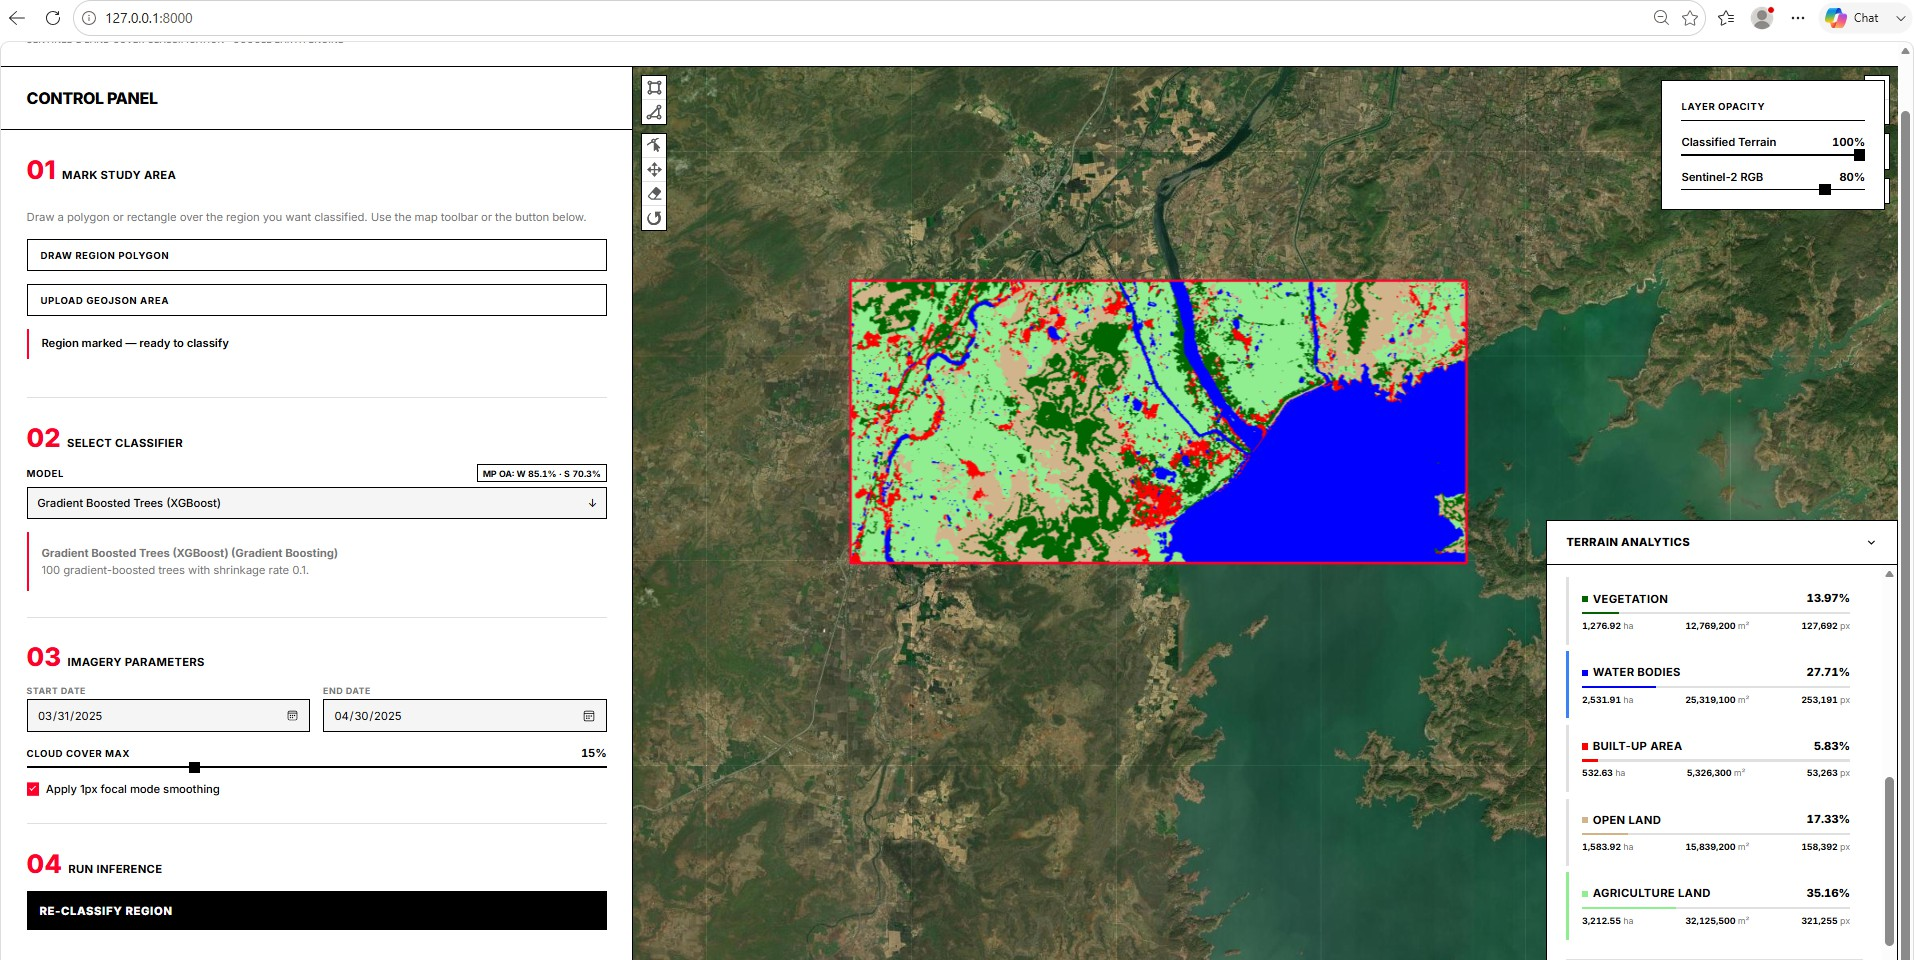
\includegraphics[width=0.92\textwidth]{fig2.png}
\caption{The served web dashboard, at full page width because its own controls and legends are otherwise unreadable in print. The left panel marks a study polygon and chooses a model (here Smile GTB); the map shows the Sentinel-2 background and the five-class overlay for the drawn area; layer opacity and class-area statistics are on the right. The raster shown here is the majority-filtered product, whose agreement is measured separately in Section~\ref{sec:delivered}.}
\label{fig:dashboard}
\end{figure*}

\FloatBarrier
\section{Methodology}
The workflow has six steps (Fig.~\ref{fig:methodology}). Satellite images are cleaned, 19 features are computed, five models are trained on labelled Jabalpur points, the chosen model is applied to the study area, and every headline accuracy figure is measured on independent public-map samples over the 29 held-out test districts. The same feature code is used for training and for mapping, so a training pixel and a map pixel are built in the same way.

\begin{figure}[!htbp]
\centering
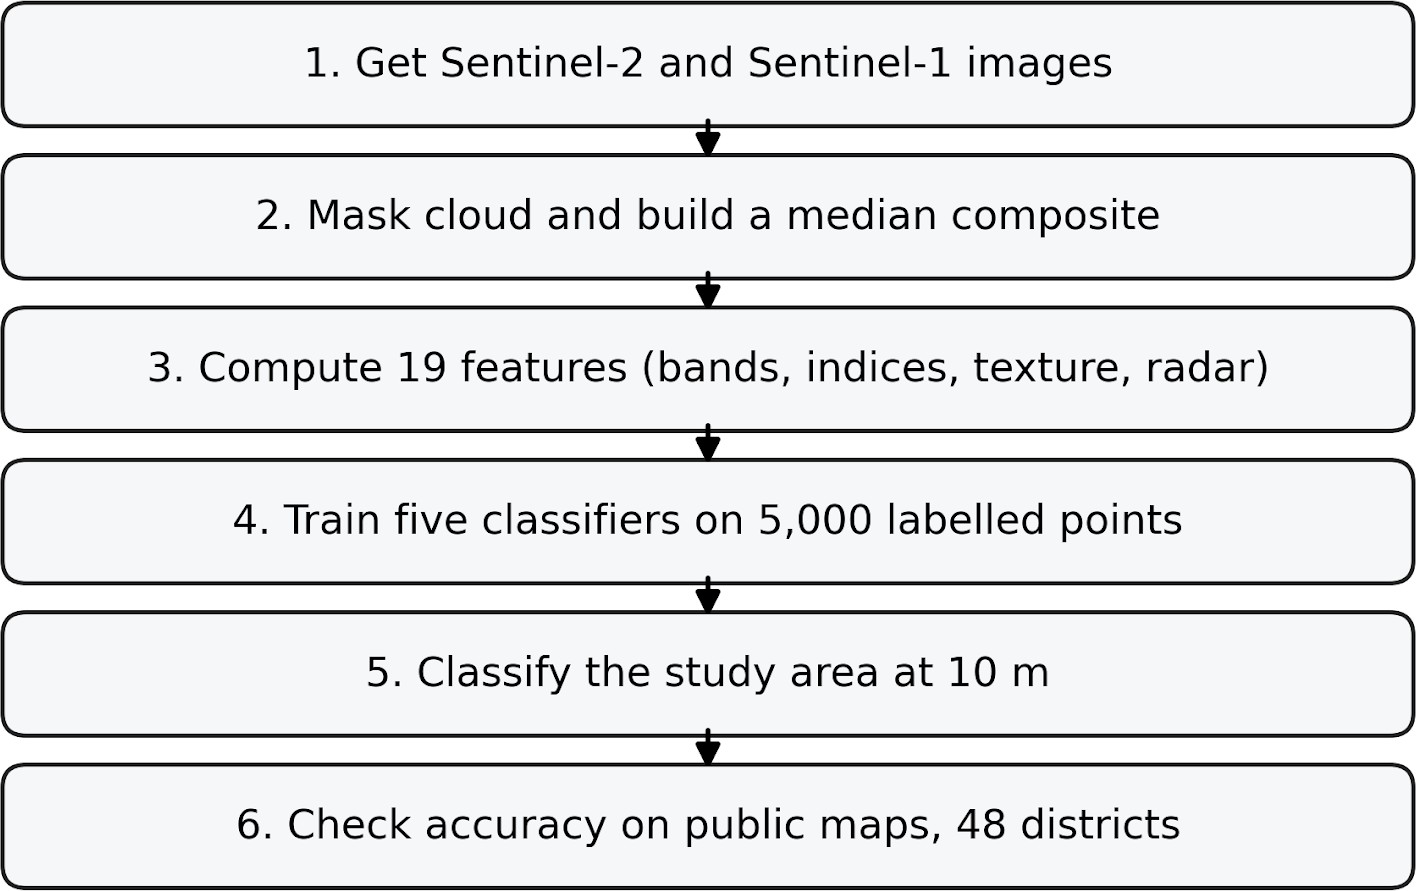
\includegraphics[width=\columnwidth]{fig3_methodology_flowchart.png}
\caption{The six steps, and the partition that decides what each number means. Twenty-seven candidate features are computed and nineteen reach the classifiers. Scoring happens against two disjoint populations: repeatedly on the 15 development districts, where every feature, model and hyperparameter choice was made, and once on the 29 test districts, which carry every accuracy this paper reports. The four districts holding labelled points are in neither.}
\label{fig:methodology}
\end{figure}

\subsection{Image cleaning}
Clouds corrupt optical reflectance. Each Sentinel-2 scene is masked with QA60 bits 10 (opaque cloud) and 11 (cirrus). A binary mask
\begin{equation}
M(x,y) = Q_{10}(x,y) \lor Q_{11}(x,y)
\end{equation}
is formed from those two bits at pixel $(x, y)$, so $M=1$ marks cloud or cirrus; pixels with $M=1$ are excluded from the median and pixels with $M=0$ contribute to it. Radar scenes in the same window are reduced by a median independently. Where the two composites are built is the only place the two lanes of Fig.~\ref{fig:methodology} differ: the training composite spans the bounding box of the labelled points, and the mapping composite spans whatever polygon is being classified. The band arithmetic that follows is one code path, so a training pixel and a map pixel are constructed identically.

An empty radar window would leave the radar bands masked and drop the affected reference points, making the loss visible in the sample count rather than hiding it in a substitution. Measured across all 48 districts and both seasons, no window is empty in either sensor.


\subsection{Features and spectral indices}
\label{sec:features}
\begin{table}[!t]
\caption{The 27 Candidate Features, and the 19 Retained by the Selected Stack}
\label{tab_bands}
\begin{center}
\setlength{\tabcolsep}{3.5pt}
\begin{tabular}{@{}L{1.5cm}L{4.3cm}c@{}}
\toprule
\textbf{Group} & \textbf{Features} & \textbf{Kept} \\
\midrule
Optical reflectance & \textbf{B4}, \textbf{B8}, \textbf{B11}, \textbf{B12}, B2, B3 & 4/6 \\
Core indices & \textbf{NDVI}, \textbf{NDWI}, \textbf{SAVI}, NDBI & 3/4 \\
Bareness, built-up & \textbf{UI}, \textbf{IBI}, \textbf{SWIRratio}, BSI, BAEI & 3/5 \\
Optical GLCM on B8 & \textbf{contrast}, \textbf{variance}, \textbf{IDM}, entropy, dissim., ASM & 3/6 \\
SAR amplitude & \textbf{VV}, \textbf{VH}, \textbf{VV$-$VH} & 3/3 \\
SAR GLCM on VV & \textbf{contrast}, \textbf{variance}, \textbf{entropy} & 3/3 \\
\midrule
\multicolumn{2}{@{}l}{\textbf{Total}} & \textbf{19/27} \\
\bottomrule
\end{tabular}

\vspace{2pt}
\parbox{\columnwidth}{\footnotesize Bold features are the 19 retained by the selected stack of Section~\ref{sec:stacks}, used for every accuracy figure in this paper. The other eight are computed on the same composite and enter the ablations of Section~\ref{sec:families} but are not given to the reported classifiers. All features are delivered on a 10\,m output grid; B11, B12 and everything derived from them carry no detail finer than their native 20\,m.}
\end{center}
\end{table}
Twenty-seven features are computed on every composite and nineteen of them go into the reported classifiers (Table~\ref{tab_bands}). The eight left out are B2, B3, NDBI, BSI, BAEI and three of the six optical GLCM measures (entropy, dissimilarity and angular second moment). Of the two dropped reflectance bands only B3 still enters the selected stack indirectly, through NDWI and IBI; B2 appears only in BSI and BAEI, both of which are also dropped, so nothing in the reported classification reads it. Which eight to drop was decided on the development districts alone, by the procedure of Section~\ref{sec:stacks}, and the full 27 are retained here so that the ablations of Section~\ref{sec:families} have something to ablate.

The indices are defined as follows. B2, B3, B4, B8, B11 and B12 are Sentinel-2 surface reflectance in $[0,1]$. NDVI (Normalised Difference Vegetation Index) \cite{r1}, \cite{r2} is $(B8-B4)/(B8+B4)$; green plants reflect near infrared and absorb red. NDWI (Normalised Difference Water Index) \cite{r22} is $(B3-B8)/(B3+B8)$. Water absorbs near infrared, so the index is high over open water. NDBI (Normalised Difference Built-up Index) \cite{r21} is $(B11-B8)/(B11+B8)$. Built surfaces are often brighter in SWIR than in NIR. SAVI (Soil-Adjusted Vegetation Index) \cite{r24} is $1.5(B8-B4)/(B8+B4+0.5)$. The extra term reduces soil brightness in sparse cover. BSI (Bare Soil Index) \cite{r25} uses blue, red, NIR and SWIR:
\begin{equation}
\text{BSI} = \frac{(B11+B4)-(B8+B2)}{(B11+B4)+(B8+B2)}
\end{equation}
It rises where soil is exposed. UI (Urban Index) \cite{r29} is $(B12-B8)/(B12+B8)$, a SWIR-NIR contrast aimed at built materials. IBI (Index-based Built-up Index) \cite{r23} is built from three normalised ratios of reflectance. Writing
\begin{equation}
u = \frac{2B11}{B11+B8}, \qquad
v = \frac{B8}{B8+B4} + \frac{B3}{B3+B11},
\end{equation}
the index is
\begin{equation}
\text{IBI} = \frac{u - v}{u + v}.
\end{equation}
It is meant to pick built land against vegetation and water, not against dry open land \cite{r26}. SWIRratio is $B11/(B12+\epsilon)$, with $\epsilon = 10^{-6}$ throughout; the SWIR slope differs slightly between soil and some built roofs. BAEI (Built-up Area Extraction Index) \cite{r30} is $(B4+0.3)/(B3+B11+\epsilon)$, a simple built-area contrast used as an extra cue.

GLCM texture \cite{r20} describes how grey levels sit next to each other in a neighbourhood. It is computed with Earth Engine's \texttt{glcmTexture} at \texttt{size}~$=3$. That argument is a radius and not a window width, so the footprint is $7\times7$ pixels; the function averages over its four directional offsets, and it is evaluated on whatever pixel grid the request establishes, which Section~\ref{sec:texture_grid} measures rather than assumes. The two grey-level images are quantised to the 32 integer levels 0--31: B8 is mapped linearly over reflectance $[0, 0.5]$ and VV over $[-25, 5]$\,dB, each clamped, so values beyond those bounds are tied to an end level before any co-occurrence is counted. Contrast, variance and dissimilarity are high on broken urban fabric; angular second moment and inverse difference moment are high on smooth open land. Texture is in the stack because a single pixel of dry soil and a single pixel of concrete can have the same colour, but a neighbourhood of roofs is rough and a neighbourhood of soil is not.

Features whose natural range is neither bounded nor comparable to reflectance are mapped onto $[0,1]$ before any classifier sees them. What is implemented is a table of twelve fixed constants, not a percentile computed at run time, and the two are worth separating because only the first is part of the trained pipeline. For the GLCM outputs, SWIRratio and BAEI the lower bound is exactly zero---these quantities are non-negative, so the 1st percentile was not used---and the upper bound is the 99th percentile of the winter labelled sample (Section~\ref{sec:labels}) rounded outward to the value printed in Table~\ref{tab_scales}; the three radar amplitude bands use the fixed decibel bounds of Section~\ref{sec:s1}. Values outside the bounds are clamped. Reflectance and the normalised-difference indices are already bounded and are left alone. The constants are frozen in \texttt{FEATURE\_RANGES} and reused unchanged by every experiment in this paper, which has one consequence that has to be declared: in the labelled-fold protocols of Section~\ref{sec:protocols} the scaling was not refitted on each fold's training rows, so the bounds were derived from a sample that includes the held-out rows. The leak is small---nine upper bounds rounded from percentiles of 5,000 rows---but it is a leak, and it inflates both protocols equally rather than the contrast between them. Without that step raw GLCM variance, which reaches about 143, dominates Euclidean distance, and SVM and KNN effectively ignore the optical and radar evidence. Table~\ref{tab_scales} lists the bounds themselves, because they are part of the trained pipeline and not a presentational choice: a reader who wants to reproduce a prediction needs them as much as the tree count.

Those bounds are fitted on the winter sample and reused unchanged in summer, which puts the two seasons on one scale and is also an asymmetry that has to be measured rather than assumed harmless. A summer distribution running hotter than its winter bound is clipped, and clipped values are tied. Section~\ref{sec:seasonal_support} reports how much of each band each season actually loses to that clipping, alongside the per-pixel observation counts the two composites rest on.

\begin{table}[!htbp]
\caption{Scaling Bounds Applied Before Every Classifier, Fitted on the Winter Labelled Sample and Reused in Summer}
\label{tab_scales}
\begin{center}
\setlength{\tabcolsep}{4pt}
\begin{tabular}{@{}lrrl@{}}
\toprule
\textbf{Feature} & \textbf{Lower} & \textbf{Upper} & \textbf{Source of the bound} \\
\midrule
SWIRratio    & 0.0 & 2.5  & winter p99 of the labelled sample \\
BAEI         & 0.0 & 9.0  & winter p99 of the labelled sample \\
\texttt{g\_contrast} & 0.0 & 22.0 & winter p99 of the labelled sample \\
\texttt{g\_ent}      & 0.0 & 4.2  & winter p99 of the labelled sample \\
\texttt{g\_var}      & 0.0 & 42.0 & winter p99 of the labelled sample \\
\texttt{g\_diss}     & 0.0 & 3.6  & winter p99 of the labelled sample \\
\texttt{s\_contrast} & 0.0 & 13.5 & winter p99 of the labelled sample \\
\texttt{s\_var}      & 0.0 & 34.0 & winter p99 of the labelled sample \\
\texttt{s\_ent}      & 0.0 & 4.0  & winter p99 of the labelled sample \\
\midrule
VV  & $-25$\,dB & $5$\,dB  & fixed decibel bounds \\
VH  & $-30$\,dB & $0$\,dB  & fixed decibel bounds \\
VV$-$VH & $-5$\,dB & $20$\,dB & fixed decibel bounds \\
\bottomrule
\end{tabular}

\vspace{2pt}
\parbox{\columnwidth}{\footnotesize Every listed feature is mapped linearly onto $[0,1]$ between its bounds and then clamped. The lower bound of every percentile-derived row is exactly zero rather than a 1st percentile, and the upper bound is a winter p99 rounded outward to the printed value; both are stored as constants and are not recomputed per run or per fold. The bounds come from the class-balanced labelled sample and not from a district-wide pixel sweep: districts are mostly vegetation and cropland, so a district p99 understates a built-up index badly on the class-balanced set the classifier actually sees. BAEI measured 2.7 on districts against 8.1 on the training samples, and a bound of 3.0 tied 12\% of winter rows to a single value.}
\end{center}
\end{table}

\subsection{What grid the texture bands were computed on}
\label{sec:texture_grid}
A GLCM neighbourhood is a number of pixels, so its footprint in metres is a property of the grid underneath it, and that grid was not documented by the statement that the classification is delivered at 10\,m. It has now been measured at every stage, because Earth Engine makes the answer non-obvious: a single Sentinel-2 scene carries EPSG:32644 at 10\,m for B8 and 20\,m for B11, but the median composite of many scenes carries the default WGS84 projection with a one-degree transform, a nominal scale of 111{,}319\,m, and every band derived from it inherits that. An image with a default projection is evaluated in the projection of the \emph{request}, so the texture footprint is set at the call site rather than in the feature code.

Two measurements settle what that means here. First, sampling the stack at \texttt{scale}~$=10$ returns texture values identical, to within $10^{-6}$ on the rescaled $[0,1]$ range over 60 test points, to those from a pipeline whose optical grey-level image is pinned to an explicit 10\,m grid with \texttt{reproject}. Training and evaluation both request 10\,m, so both saw \texttt{glcmTexture(size=3)} as a $7\times7$ window on a 10\,m grid: a 70\,m footprint, which is what every reported result rests on. Second, the footprint does follow the request. Sampling the same points at 20, 30, 60 and 100\,m moves optical GLCM contrast by a mean of 0.073, 0.158, 0.239 and 0.292 on its rescaled $[0,1]$ range, moves SAR contrast further, and changes the predicted class of 1, 3, 2 and 4 of the 60 points; pinning the optical grey-level image to a 30\,m grid and still sampling at 10\,m changes the three optical texture bands and 6 of the 60 predictions, while leaving the radar texture, which that pinning does not touch, unchanged.

That has no effect on the numbers in this paper and a direct one on the map the dashboard serves. The renderer asks for the drawn polygon's width in metres divided by ten, capped at 2{,}048 pixels, so an area up to about 20\,km wide is rendered on the 10\,m grid the model was fitted for, and anything larger is not: a 50\,km polygon is classified at 24.4\,m and a 200\,km one at 97.7\,m, giving GLCM footprints of 171\,m and 684\,m against the 70\,m of training. The delivered product for a large area is therefore not the assessed product, which Section~\ref{sec:delivered} takes up. \texttt{texture\_grid\_audit.json} carries the projection of every stage and the full scale sweep.

\subsection{Land-cover classes and labelled points}
\label{sec:labels}
Five classes are used throughout this paper, the dashboard and the GEE assets:
\begin{itemize}
    \item \textbf{Vegetation (label 0):} trees, dense foliage and other green cover.
    \item \textbf{Water (label 1):} rivers, lakes, ponds and other open water.
    \item \textbf{Built area (label 2):} buildings, roads and other constructed surfaces.
    \item \textbf{Open land (label 3):} bare rock, exposed soil and unvegetated ground.
    \item \textbf{Agriculture (label 4):} cultivated fields, seasonal crops and fallow farmland.
\end{itemize}

To provide sharper operational definitions, Table \ref{tab_ontology} lists inclusion and exclusion rules for difficult cases.

\begin{table}[!b]
\caption{Class Ontology Decision Rules and Difficult Cases}
\begin{center}
\begin{tabular}{p{2cm}p{3cm}p{2.5cm}}
\toprule
\textbf{Class} & \textbf{Includes} & \textbf{Excludes} \\
\midrule
Vegetation & Orchards, plantations, forests, urban parks & Seasonal crops \\
Water & Rivers, lakes, ponds & Dry riverbeds (Open) \\
Built area & Concrete, asphalt, buildings, roads & Construction sites (Open) \\
Open land & Bare soil, rocky outcrops, dry riverbeds, construction sites & Fallow cropland (Agri.) \\
Agriculture & Fallow cropland, harvested fields, seasonal crops & Plantations (Veg.) \\
\bottomrule
\end{tabular}
\label{tab_ontology}
\end{center}
\end{table}

Exactly 1,000 manually placed points were prepared per class, 5,000 in total, the counts verified against the point collections themselves. Two further counts belong beside that one, because a label count is not a count of independent evidence: the 5,000 features occupy 4,998 distinct coordinates, two being exact duplicates, and 4,988 distinct cells on the 10\,m grid the features are sampled at, so ten further pairs share a pixel with another point of the same class. Labels were placed by visual interpretation of 2025 Sentinel-2 composites and Google Earth very-high-resolution basemaps. Measured against the Jabalpur polygon, 872 of the 5,000 points fall outside it: 868 in Katni, 3 in Dindori, 1 in Mandla, every one within 23\,km of the boundary. Katni was separated from Jabalpur in 1998, so a wider historical outline explains the placement, but under the boundaries used for evaluation those three districts hold training data, and they are withheld from all reported accuracy together with Jabalpur itself. The points are tightly clustered. The median nearest-neighbour distance within a class ranges from 29\,m (open land) to 371\,m, and 984 of the 1,000 open-land points lie within 100\,m of another point of the same class. On a 10\,m grid 100\,m is ten pixels and the 29\,m median is under three. That clustering is the mechanism behind the inflated random-split accuracy of Table~\ref{tab_protocols}, discussed in Section~\ref{sec:protocols}. No formal double-annotation by a second interpreter was performed, and the assets carry no interpreter, source-image or date attribute, so per-point provenance cannot be reconstructed. Each point carries its own integer label. Pixel values are read with GEE \texttt{sampleRegions} on a 10\,m output grid. That is an output grid and not a uniform native resolution: B11 and B12 are acquired at 20\,m and QA60 at 60\,m, and Earth Engine resamples them by nearest neighbour when the request specifies 10\,m, so a 10\,m pixel of B11 carries no information finer than 20\,m. Five of the nineteen model inputs derive from the 20\,m bands. Rows with a missing label or a missing band are dropped. The training composite is the bounding box of the points themselves, so no labelled point can fall outside the stack it is sampled from.

The sampled table is audited per season rather than assumed intact. All 27 candidate features are computed for every point, and all 5,000 rows survive the \texttt{notNull} filter in both seasons, 1,000 in each class: no row is lost to a masked optical band or an empty radar window, so the two seasons train on the same rows and a seasonal difference in accuracy cannot be a seasonal difference in training size. Those counts are asserted before training, not checked afterwards.

Label integrity is enforced rather than assumed. \texttt{sampleRegions} drops rows whose label is null without raising, so a collection that has lost its attributes contributes zero training rows and the model simply trains on fewer classes. Every source asset therefore carries its own label attribute, and a pre-training audit asserts the expected label histogram and point count per asset. A schema version string is stamped into every stored result so that runs computed under different class inventories cannot be merged.

\subsection{Classifiers}
Five supervised machine-learning algorithms were selected for their prominence in remote sensing literature and their native server-side implementation within Google Earth Engine (Table~\ref{tab_hyper}). Each algorithm employs a fundamentally different mathematical approach to partition the feature space, allowing for a comprehensive comparison of classification strategies:
\begin{enumerate}
    \item \textbf{Random Forest (RF):} An ensemble learning method \cite{r11} that constructs a multitude of decision trees during training and outputs the mode of the classes. It introduces randomness by bagging (training each tree on a bootstrapped sample) and randomly selecting a subset of features at each split, making RF highly resistant to overfitting. It is implemented with \texttt{ee.Classifier.smileRandomForest}.
    \item \textbf{Support Vector Machine (SVM):} SVM \cite{r12} locates the optimal separating boundary (hyperplane) that maximizes the margin between classes in the feature space. We used the Radial Basis Function (RBF) kernel to implicitly map inputs into higher-dimensional spaces for complex, non-linear distributions. It is implemented with \texttt{ee.Classifier.libsvm}.
    \item \textbf{Smile GTB:} gradient tree boosting \cite{r27} builds trees sequentially, each new tree fitting the residual errors of the ensemble so far. Earth Engine exposes the Smile library's implementation as \texttt{ee.Classifier.smileGradientTreeBoost}, which is what this study uses. The three arguments searched here---tree count, shrinkage rate and node cap---are its capacity controls, not the whole of its interface: it also takes a sampling rate, a loss function and a seed, which are left at their defaults and reported as such in Table~\ref{tab_hyper}. Results obtained with it should not be reported under the name of another boosting implementation \cite{r13}.
    \item \textbf{CART:} Classification and Regression Trees construct a single decision tree by recursively partitioning the feature space using binary splits based on information gain. While highly interpretable, a single CART model is prone to overfitting. It serves as a baseline, implemented with \texttt{ee.Classifier.smileCart}.
    \item \textbf{k-Nearest Neighbours (KNN):} KNN classifies a pixel based on the majority vote among its $k$ closest training samples using Euclidean distance. As a non-parametric method, it is sensitive to features with large numerical ranges, necessitating our rigorous normalisation step. It is implemented with \texttt{ee.Classifier.smileKNN}.
\end{enumerate}
The trained model is applied to any polygon. A $3\times3$ majority filter removes isolated speckle. Outputs are class areas, a tiled PNG overlay and a GeoTIFF. The filter is a cartographic post-process on the delivered product only: every accuracy figure in this paper is computed on the unfiltered per-pixel classification, so none of them borrows the smoothing that the map a user sees has received. The consequence runs the other way as well: the filtered raster the dashboard serves is a different product from the one every accuracy here describes, and the class areas it yields differ from the raw ones, which is why Fig.~\ref{fig:jabalpur_map} lists both. It is measured separately in Section~\ref{sec:delivered} rather than assumed equivalent.

\begin{table}[!htbp]
\caption{Classifier Settings, Selected on the 15 Development Districts and Then Frozen}
\label{tab_hyper}
\begin{center}
\setlength{\tabcolsep}{3.5pt}
\begin{tabular}{lp{3.0cm}p{3.1cm}}
\toprule
\textbf{Classifier} & \textbf{Grid searched} & \textbf{Selected} \\
\midrule
Random Forest & trees $\{100,300\}$, max nodes $\{10,50,\text{none}\}$ & 300 trees, bag fraction 0.5, min leaf 1, no node cap \\
SVM           & cost $\{10,100\}$, $\gamma\in\{0.1,0.5,1.0\}$ & RBF kernel, cost 10, $\gamma=0.1$ \\
Smile GTB     & trees $\{100,300\}$, shrinkage $\{0.05,0.1\}$, max nodes $\{10,50\}$ & 300 trees, shrinkage 0.1, max nodes 10 \\
CART          & max nodes $\{10,20,50,\text{none}\}$ & max nodes 20 \\
KNN           & $k\in\{3,5,9,15\}$ & $k=9$ \\
\bottomrule
\end{tabular}

\vspace{2pt}
\parbox{\columnwidth}{\footnotesize Twenty-eight configurations in total per season, summed across the five models. Each model's configuration is the one with the highest winter development accuracy, and the same configuration is used in both seasons and in the dashboard. Bag fraction 0.5 and min leaf population 1 were held fixed for Random Forest. Arguments not listed are left unset and therefore take the Earth Engine defaults, which are part of the trained pipeline even though they were not searched: for Smile GTB that is a sampling rate of 0.7 and seed 0, and for Random Forest seed 0. Smile GTB exposes further arguments than the three searched here; the three are the capacity controls, and the others were not exercised.}
\end{center}
\end{table}

\subsection{How accuracy is measured}
\label{sec:accuracy}
Project labels are used for training, and every headline accuracy figure in this paper is instead agreement with an independent reference. The single exception is the two labelled-set protocols of Table~\ref{tab_protocols}, which deliberately score the project's own labels in order to measure what the validation protocol is worth; those rows are never quoted as the accuracy of the method. The screening rule is class-specific rather than uniform, and the exact Boolean condition implemented for each of the five classes is given below, transcribed from \texttt{evaluation/references.py} of the released code. $\mathrm{WC}$ is the ESA WorldCover \cite{r14} class code; $\mathrm{DW}$ is the Dynamic World \cite{r15} class whose mean probability over the season window is highest, taken as the arg-max of the nine per-class mean probability bands rather than as a modal label; $p_{\mathrm{DW}}$ is that mean probability; and the specialist layers are OPERA DSWx for water, the GHSL built-surface layer for built area (at least $50\text{ m}^2$ of built surface inside the $100\text{ m}^2$ of a 10\,m cell, that is a built fraction of one half or more), and WorldCereal \cite{r16} for agriculture:
\begin{equation}
\small
\begin{aligned}
\text{Vegetation}  \;&:\; \mathrm{WC}{=}10 \wedge \mathrm{DW}{=}1 \wedge p_{\mathrm{DW}}\!\ge\!0.70 \\
\text{Water}       \;&:\; \mathrm{WC}{=}80 \wedge \mathrm{DW}{=}0 \wedge p_{\mathrm{DW}}\!\ge\!0.70 \wedge \mathrm{OPERA} \\
\text{Built area}  \;&:\; \mathrm{WC}{=}50 \wedge \mathrm{DW}{=}6 \wedge p_{\mathrm{DW}}\!\ge\!0.70 \wedge \mathrm{GHSL} \\
\text{Open land}   \;&:\; \mathrm{WC}{=}60 \wedge \mathrm{DW}{=}7 \wedge \neg\,\mathrm{specialist} \\
\text{Agriculture} \;&:\; \mathrm{WC}{=}40 \wedge \mathrm{WorldCereal}
\end{aligned}
\label{eq:refrules}
\end{equation}
Two of these five rows are weaker than the other three, and the difference is material to every number in this paper. Open land carries the Dynamic World \emph{label} but not the 0.70 confidence threshold, so a low-confidence bare pixel can enter the reference where a low-confidence tree pixel cannot. Agriculture carries neither: it requires only that WorldCover call the pixel cropland and that WorldCereal call it temporary crops, with Dynamic World taking no part in the decision. The reference is therefore a set of class-specific screens and not the single high-confidence consensus a uniform rule would produce, and the classes are not screened at equal strictness. Section~\ref{sec:limits} carries the consequence: because agriculture is the least strictly screened class and also the largest by area, class coverage, class-conditional reference error and the area weights of Section~\ref{sec:area} all inherit this asymmetry, and no experiment reported here separates a classifier error from a reference-screening artefact. Disagreement under whichever rule applies is left out of the reference rather than guessed.

Agreement between two products with different legends is only defined once those legends are mapped onto the five classes, so Table~\ref{tab_crosswalk} gives that mapping. It is deliberately incomplete. WorldCover grassland and Dynamic World grass and shrub have no unambiguous home in an inventory whose vegetation class is woody and whose agriculture class is cultivated, so they are assigned to no class and a pixel carrying either of them can never enter the reference. The same is true of snow, ice and moss, which do not occur in the study area. This is the main reason the consensus domain covers only part of the state, and it is why the area-weighted figures of Section~\ref{sec:area} describe that domain rather than Madhya Pradesh.

Each reference layer is used at a fixed epoch and on its own native grid, and both matter. WorldCover is v200, whose observation year is 2021, at 10\,m. WorldCereal is the 2021 v100 \texttt{temporarycrops} product at 10\,m, mosaicked over the study area and used unchanged in both windows. The seasonal active-cropland markers were evaluated first and returned no valid pixels over Madhya Pradesh in either window, so the annual temporary-crops layer stands in their place. The consequence is larger than one layer, because the agriculture row of Eq.~\eqref{eq:refrules} consults nothing else that moves: WorldCover v200 is a fixed 2021 epoch, WorldCereal is a fixed 2021 annual product, and Dynamic World takes no part in that row at all. The agriculture stratum is therefore \emph{static in its entirety}, not merely static in its specialist. Its eligible area is the same 167{,}250.56\,km$^2$ over the 48 districts in both windows and identical district by district in all 48 of them, and because the stratified draw is seeded on an identical mask it returns the same agriculture locations in both seasons. Nothing in the agriculture reference is seasonal; only the imagery read at those fixed locations is, which is what makes the fixed-location control of Section~\ref{sec:fixed} possible. The GHSL built-surface layer is P2023A, whose observation epoch is 2018, at 10\,m. OPERA DSWx-HLS is posted at 30\,m, so the water specialist is the one condition in the consensus that cannot resolve a 10\,m cell and instead carries its 30\,m neighbourhood's water classification. The ESRI arbiter is the 2024 annual product at 10\,m. Dynamic World alone is composited over the same season window as the classification it checks, because it is a per-scene product. Every one of these identifiers, with its epoch, grid and remap, is listed in \texttt{reference\_inventory.csv} of the result archive. The epoch spread---2018 for built surface, 2021 for two of the general products, 2024 for the arbiter, 2025 for the imagery---is a real source of apparent error, bounded against the arbiter below and carried into the limitations rather than corrected.

\begin{table*}[!t]
\caption{Crosswalk from the Reference Products to the Five Classes}
\label{tab_crosswalk}
\begin{center}
\begin{tabular}{@{}L{2.2cm}L{5.4cm}L{4.2cm}L{4.6cm}@{}}
\toprule
\textbf{Class} & \textbf{WorldCover v200} & \textbf{Dynamic World} & \textbf{Specialist} \\
\midrule
Vegetation  & tree cover (10) & trees (1), $p\ge0.70$ & --- \\
Water       & permanent water (80) & water (0), $p\ge0.70$ & OPERA DSWx \\
Built area  & built-up (50) & built (6), $p\ge0.70$ & GHSL $\ge$ 1/2 \\
Open land   & bare / sparse (60) & bare (7), \emph{no threshold} & none may claim \\
Agriculture & cropland (40) & \emph{not used} & WorldCereal \\
\midrule
\emph{unassigned} & grassland (30), shrubland (20), herbaceous wetland (90), mangroves (95), snow/ice (70), moss (100) & grass (2), crops (4), shrub \& scrub (5), flooded veg.\ (3), snow/ice (8) & --- \\
\bottomrule
\end{tabular}

\vspace{2pt}
\parbox{\textwidth}{\footnotesize This table is the executable rule of Eq.~\eqref{eq:refrules} and not a summary of it; each row is exactly the mask built in \texttt{evaluation/references.py}. The screening is not uniform across rows. Three classes require WorldCover, the matching Dynamic World label and a Dynamic World probability of at least 0.70; open land requires the label but no probability threshold; agriculture requires WorldCover and WorldCereal and consults Dynamic World not at all. Wetland, flooded vegetation and mangrove codes are \emph{unassigned} rather than folded into water or vegetation, so no pixel carrying them can enter the reference. Exclusion by the unassigned row is not symmetric between the two general products, and the asymmetry is the same one the rest of this table records. Every row requires a specific WorldCover code, so a pixel whose WorldCover label is unassigned can enter no class. A pixel whose \emph{Dynamic World} label is unassigned is excluded from vegetation, water, built area and open land, but not from agriculture, which never reads Dynamic World: a Dynamic World grass or shrub pixel that WorldCover calls cropland and WorldCereal calls temporary crops enters the reference as agriculture. Unassigned WorldCover codes are the main reason the covered domain does not reach the whole state, and the Dynamic World conditions are the main reason the part it does cover is dominated by one class.}
\end{center}
\end{table*}

Sampling is 20 points per class per district at 10\,m over all 48 district polygons. Any candidate within 100\,m of a training point is removed. Because every training point lies inside the four districts that are withheld in the next step, this buffer removes nothing from the reported test half; it is retained so that the development and test samples are constructed by the same procedure as the withheld districts. The four districts that contain training points are then withheld entirely, and the remainder is split by spatial block into 15 development and 29 test districts (Table~\ref{tab_splits}, Fig.~\ref{fig:split_map}). The quota is a ceiling and not a guarantee, because a district need not contain 20 pixels of every class that clear the consensus. After the buffer and the split, 2,900 winter and 2,692 summer reference points remain in the test half, and 1,500 winter and 1,418 summer in the development half. The two winter counts are exactly $20\times5\times29$ and $20\times5\times15$: in winter the quota was met in every class of every district. Summer falls 208 points short in the test half and 82 in the development half. Those missing points are not spread across the classes and do not come from agriculture or open land: \emph{every one of the 208 is vegetation}. The summer test sample holds 372 vegetation points against 580 of each of the other four classes, and the winter sample holds 580 of all five. The eligible vegetation area inside the test districts falls from 2,039\,km$^2$ in winter, 1.90\% of the covered domain, to 121\,km$^2$ in summer, 0.12\% of it. That is the background condition and not by itself an explanation, so Table~\ref{tab_shortfall} audits the twelve short strata district by district on the same 10\,m grid the sample is drawn on. Every one of the twelve holds fewer than twenty eligible vegetation pixels, eight of them none at all, and in the four that hold any the sampler returned as many points as there were pixels to find, or one more where a boundary pixel falls between the two measurements. The shortfall is therefore scarcity in the reference and not a property of the sampler.

That conclusion depends on the grid. Measured at 30\,m, as an earlier version of this paper measured its stratum areas, Bhind appears to hold about 4{,}400 eligible vegetation pixels while returning none, which invites exactly the wrong explanation; on the 10\,m grid the sample is actually drawn on, Bhind holds none. A coarse area measurement manufactures eligible area for a class that survives only in scattered single pixels, and the shortfall audit is one of the places where that shows. Which class the shortfall falls on matters, because vegetation is also the class whose summer recall is weakest at 44.09\%.
\begin{table}[!htbp]
\caption{Every Test Stratum that Missed the 20-Point Quota. All Twelve are Summer Vegetation; Winter Missed None}
\label{tab_shortfall}
\begin{center}
\setlength{\tabcolsep}{4pt}
\footnotesize
\begin{tabular}{@{}lrrr@{}}
\toprule
\textbf{District} & \textbf{km$^2$} & \textbf{Pixels} & \textbf{Drawn} \\
\midrule
Raisen     & 0.0013 & 13 & 14 \\
Vidisha    & 0.0007 & 7 & 8 \\
Chhatarpur & 0.0006 & 6 & 7 \\
Panna      & 0.0003 & 3 & 3 \\
Bhind, Burhanpur, Dewas, E.\ Nimar, & \multirow{2}{*}{0.0000} & \multirow{2}{*}{0} & 0, 0, 0, 0, \\
Gwalior, Morena, Ratlam, Ujjain & & & 0, 0, 0, 0 \\
\bottomrule
\end{tabular}

\vspace{2pt}
\parbox{\columnwidth}{\footnotesize ``Pixels'' converts the eligible area, measured on the 10\,m sampling grid, to 10\,m cells. The drawn count exceeds the measured pixel count by one in three rows, which is the resolution of a boundary pixel rather than a sampling anomaly. No stratum here holds twenty eligible pixels, so no draw could have met the quota. From \texttt{reference\_shortfall\_audit.json}.}
\end{center}
\end{table}

This has a direct consequence for how the summer headline figure may be described. With one class at 372 points and four at 580, the pooled summer accuracy is no longer class-balanced. Pooled summer agreement is 73.85\%, and the class-balanced figure, the unweighted mean of the five per-class recalls, is 71.71\%. Both are reported throughout: the winter sample is exactly balanced so its two figures coincide at 87.41\%, and only in summer do they separate. The seasonal gap is therefore 15.70 points on the class-balanced reading rather than the 13.56 points a pooled-to-pooled comparison suggests, and neither number is a fixed-location comparison, since the two seasons do not sample the same reference domain. Summer accuracy is therefore measured on a slightly smaller and slightly differently composed sample than winter, which is a further reason not to read the seasonal gap as a pure phenology effect. 
We report overall accuracy (OA), Cohen's Kappa \cite{r28} and per-class F1, with per-class precision and recall given for the two classes that carry the argument (Table~\ref{tab_families}). Every one of those is computed from the stored confusion matrix $C$ and from nothing else, by the identities $n=\sum_{ab} C_{ab}$, $\mathrm{OA}=\mathrm{tr}(C)/n$, $\mathrm{recall}_a = C_{aa}/\sum_b C_{ab}$, $\mathrm{precision}_a = C_{aa}/\sum_b C_{ba}$ and $F1_a = 2C_{aa}/(\sum_b C_{ab} + \sum_b C_{ba})$, with Kappa taken from the same matrix and its marginals. The archive rebuild asserts each identity for every matrix it prints a metric from, so a table and a figure cannot disagree about the same run. Kappa is reported because the LULC literature this work is compared against reports it, not because it adds information beyond OA; Olofsson et al.\ \cite{r17} recommend against it, and no conclusion here rests on it.

\subsection{Area-weighted agreement over the covered domain}
\label{sec:area}
The sample above takes 20 points per class per district, so it describes a landscape in which the five classes are equally common. They are not. An overall accuracy read off that sample answers a question about the sample design; a question about ground needs the strata weighted by the area they occupy. The estimator below is the standard stratified one \cite{r17}, and what it estimates has to be stated as carefully as how it is computed, because it is not statewide accuracy.

\subsubsection{Population and strata}
For season $s$, let $\mathcal{C}_s$ be the set of pixels in the 29 test districts that pass the consensus and specialist rules of Table~\ref{tab_crosswalk}. This is the covered reference domain, and it is smaller than the test districts: it is 107,437\,km$^2$ of their 190,330\,km$^2$ in winter (56.5\%) and 104,670\,km$^2$ (55.0\%) in summer. Nothing outside it is assessed by any figure in this paper. A stratum $h$ is one (district, consensus class) cell, which is exactly the unit the sample was drawn by. Its eligible area is $A_h$, measured on the same 10\,m grid the sample is drawn on and under the same masks that build the reference, its sample count is $n_h$, and its weight is $W_h = A_h/\sum_h A_h$. There are 145 strata in winter and 137 in summer.

The grid the areas are measured on is part of the estimator and not an implementation detail, which an earlier version of this paper treated it as. Measuring at 30\,m for a sample drawn at 10\,m under-measures whichever classes are fragmented, and it did: recomputing on the sampling grid raises built area's share of the winter domain from 0.29\% to 0.30\% and vegetation's from 1.86\% to 1.90\%, lowers agriculture's from 95.92\% to 95.86\%, and raises weighted user's accuracy for built area from 3.29\% to 3.43\% and for vegetation from 32.33\% to 32.75\%. The weighted overall estimate is unmoved at 75.50\%, so the conclusions drawn from it did not depend on the grid; two accounting defects that did depend on it are gone, as the next paragraph records.

\subsubsection{Estimator}
Let $z_{hi}=1$ when the prediction and the consensus label agree for sampled pixel $i$ in stratum $h$, and 0 otherwise. Then
\begin{equation}
\widehat{\mathrm{OA}}_{\mathcal{C}} = \sum_h W_h \, \bar{z}_h,
\qquad
\bar{z}_h = \frac{1}{n_h}\sum_{i=1}^{n_h} z_{hi},
\label{eq:oac}
\end{equation}
and the full weighted error matrix has cells
\begin{equation}
\hat{p}_{ab} = \sum_h W_h \, \frac{1}{n_h} \sum_{i=1}^{n_h} \mathbb{I}\!\left(r_{hi}=a,\; \hat{y}_{hi}=b\right),
\label{eq:pab}
\end{equation}
with $r$ the reference label and $\hat{y}$ the prediction, so that $\widehat{\mathrm{OA}}_{\mathcal{C}} = \sum_a \hat{p}_{aa}$ and the row and column margins give consensus-relative producer's and user's accuracies. The strata are defined by the reference and not by the map, so the weights come from the reference class areas and never from the classifier's own mapped proportions.

Treating each stratum as a simple random sample of its pixels, the design-based variance is
\begin{equation}
\widehat{V}\!\left(\widehat{\mathrm{OA}}_{\mathcal{C}}\right)
 = \sum_h W_h^2 \, \frac{\bar{z}_h\left(1-\bar{z}_h\right)}{n_h - 1},
\label{eq:var}
\end{equation}
and the reported $\pm$ figure is $1.96\sqrt{\widehat{V}}$. Three properties of that interval should be read with it. No finite-population correction is applied: the within-stratum sampling fraction is of order $10^{-7}$, so the correction is negligible, but it is omitted rather than absent. A stratum with $n_h < 2$ contributes its point estimate and no variance. And the interval answers a different question from the district bootstrap used elsewhere in this paper: this one says how precisely the sample pins down the agreement of a fixed mapped area, while resampling whole districts asks how much the answer depends on which districts were drawn. Both are reported and neither substitutes for the other.

Two accounting defects that the 30\,m weights carried are worth recording because they are what a mismatched grid produces. Two summer strata then had nonzero area and no sampled point, so the estimate had to be renormalised onto the area the sampled strata represented; and three summer test points fell in strata of no measured area and therefore carried no weight, leaving the summer weighted estimate resting on 2,689 of the 2,692 points the unweighted figure uses. On the sampling grid neither survives: every stratum with area has a sample, every sampled point carries weight, and both seasons use all of their points.

\subsubsection{What the two numbers are}
Table~\ref{tab_coverage} gives the pair for each season and population. The sample estimate and the area-weighted estimator address different questions.

Before either is interpreted, the composition of the weighted domain has to be stated, because it decides what a high weighted score would mean. Summing the eligible stratum areas of \texttt{stratum\_areas.csv} over the 29 test districts, the covered domain is 95.86\% agriculture by area in winter and 98.39\% in summer; vegetation, water, built area and open land share the remaining 4.14\% and 1.61\% between them, and summer vegetation is 0.12\% of it. A domain that skewed admits a trivial baseline, and it must be reported beside the estimate: a constant predictor that labels every pixel agriculture and is never trained on anything achieves an area-weighted agreement of 95.86\% in winter and 98.39\% in summer, against the trained pipeline's 75.50\% and 58.67\%. On this metric, over this domain, the trained pipeline loses to the constant baseline by 20.4 and 39.7 points.

That comparison is not evidence that the classifier is worthless, and it should not be read as one: the same predictions score 87.41\% and 73.85\% on the sample, where the same constant predictor scores 21.55\% pooled in summer, 20.00\% pooled in winter and 20.00\% class-balanced in both, and a map that calls all of Madhya Pradesh cropland has no use whatever. What the comparison does establish is that $\widehat{\mathrm{OA}}_{\mathcal{C}}$ over this domain is not a measure of practical mapping quality and cannot be quoted as one, because a degenerate map outscores a trained one on it. It is not that the estimator is maximised by the degenerate map---perfect agreement would score 100\%---but that the ranking it induces over maps is not a ranking by map quality. The weighted figure answers only how often the map agrees with the reference on the area the reference covers, in a domain the reference construction made overwhelmingly agricultural; the imbalance is an artefact of Eq.~\eqref{eq:refrules}, under which agriculture is the least strictly screened class, rather than a property of the state.

The informative version of this estimator is the per-class one, and Table~\ref{tab_weighted_class} gives it. Decomposing $\hat{p}_{ab}$ by row and column recovers the same 75.50\% and 58.67\% on the diagonal, so the decomposition is an identity and not a second measurement, and it changes what the headline can be read to mean. Weighted producer's accuracy is high for every class in winter, 87.5\% to 100\%, so the map finds the minority classes where they are. Weighted user's accuracy is not: built area is 3.43\%, open land 1.83\%, vegetation 32.75\% and water 48.42\%. In summer open land falls to 0.77\% and vegetation to 1.49\%.

The arithmetic behind that is prevalence, not a collapse in the classifier. Agriculture occupies 95.86\% of the winter domain and 25.31\% of it is given some other label; the absolute area of those false positives is many times the entire true area of built land or open land, which together hold 0.53\% of the domain. A minority class can therefore be found almost perfectly and still be swamped, and any user of a map over this domain who asks ``where the map says built, is it built'' gets a very different answer from one who asks ``how often does the map agree''. Both are properties of the reference domain's composition as much as of the classifier, and neither is a statewide statement. This is the strongest single reason the weighted overall figure should not be quoted alone.

\begin{table}[!htbp]
\caption{Area-Weighted Agreement by Class over the Covered Domain, Smile GTB, 29 Test Districts}
\label{tab_weighted_class}
\begin{center}
\setlength{\tabcolsep}{3.5pt}
\footnotesize
\begin{tabular}{@{}lrrrrrr@{}}
\toprule
 & \multicolumn{3}{c}{\textbf{Winter}} & \multicolumn{3}{c}{\textbf{Summer}} \\
\cmidrule(lr){2-4}\cmidrule(lr){5-7}
\textbf{Class} & \textbf{Area} & \textbf{Prod.} & \textbf{User} & \textbf{Area} & \textbf{Prod.} & \textbf{User} \\
 & \% & \% & \% & \% & \% & \% \\
\midrule
Vegetation  &  1.90 &  89.13 & 32.75 &  0.12 &  30.34 &  1.49 \\
Water       &  1.72 & 100.00 & 48.42 &  0.79 & 100.00 & 15.73 \\
Built area  &  0.30 &  99.61 &  3.43 &  0.37 &  99.01 &  4.17 \\
Open land   &  0.23 &  87.40 &  1.83 &  0.33 &  61.10 &  0.77 \\
Agriculture & 95.86 &  74.69 & 99.72 & 98.39 &  58.21 & 99.85 \\
\midrule
\textbf{Overall} & & \multicolumn{2}{c}{\textbf{75.50}} & & \multicolumn{2}{c}{\textbf{58.67}} \\
\bottomrule
\end{tabular}

\vspace{2pt}
\parbox{\columnwidth}{\footnotesize Computed by \texttt{scripts/weighted\_per\_class.py} from \texttt{stratum\_areas.csv} and \texttt{district\_confusion\_matrices.csv}, using the strata and weights of Eqs.~\eqref{eq:oac}--\eqref{eq:pab}. ``Area'' is the class's share of the covered domain, ``Prod.'' its weighted producer's accuracy and ``User'' its weighted user's accuracy. The diagonal of the weighted matrix sums to the overall row, which reproduces the values of Table~\ref{tab_coverage} and confirms the decomposition is exact. Summer weights are renormalised onto the sampled strata as Section~\ref{sec:area} describes.}
\end{center}
\end{table} Sample agreement gives similar weight to each reference class within a district, whereas area-weighted agreement reflects the prevalence of reference strata within the consensus-covered test domain. Neither estimate applies automatically to pixels excluded by the reference construction, and neither removes systematic errors shared by the reference products.

\begin{table}[!htbp]
\caption{Reference-Domain Coverage and the Two Agreement Estimates}
\label{tab_coverage}
\begin{center}
\setlength{\tabcolsep}{3pt}
\footnotesize
\begin{tabular}{@{}lrrrrr@{}}
\toprule
\textbf{Season, population} & \textbf{Area} & \textbf{Covered} & \textbf{$n$} & \textbf{Unwtd.} & \textbf{Wtd.} \\
 & km$^2$ & \% & & \% & \% \\
\midrule
Winter, dev.\ (15)  &  94{,}954 & 58.8 & 1{,}500 & 87.13 & 77.10 $\pm$ 4.58 \\
Winter, test (29)   & 190{,}330 & 56.5 & 2{,}900 & 87.41 & 75.50 $\pm$ 3.32 \\
Summer, dev.\ (15)  &  94{,}954 & 58.2 & 1{,}418 & 75.25 & 56.21 $\pm$ 5.60 \\
Summer, test (29)   & 190{,}330 & 55.0 & 2{,}692 & 73.85 & 58.67 $\pm$ 4.01 \\
\bottomrule
\end{tabular}

\vspace{2pt}
\parbox{\columnwidth}{\footnotesize ``Area'' is the total area of the district polygons and ``covered'' the percentage of it the consensus assigns to one of the five classes; in absolute terms that is 55{,}833 and 107{,}437\,km$^2$ in winter and 55{,}257 and 104{,}670\,km$^2$ in summer, all measured on the 10\,m sampling grid. The covered domain is the population described by the area-weighted column and the only domain assessed by those estimates. Smile GTB throughout. The area-weighted column is~\eqref{eq:oac} with the half-width $1.96\sqrt{\widehat{V}}$ of~\eqref{eq:var}; the unweighted column is the same predictions scored without weights. Both seasons' weighted estimates use every sampled point and every stratum that carries area, which the 30\,m weights did not achieve in summer. Every quantity in this table is reproduced in \texttt{reference\_domain\_coverage.csv} and \texttt{stratum\_areas.csv} of the result archive.}
\end{center}
\end{table}

The consensus reference is a useful external benchmark, but it is not equivalent to field-verified ground truth. The constituent products (WorldCover, Dynamic World, OPERA DSWx, GHSL, WorldCereal) have their own classification errors, use overlapping Sentinel inputs, and several reference epochs do not match the 2025 composites. The ESRI 2024 map provides an additional inter-product agreement check because it is not used in constructing the consensus and its epoch is the closest of any candidate to the 2025 composites. Agreement of 83.8\% in winter and 81.1\% in summer on the test reference samples (82.7\% and 80.5\% over all 44 evaluation districts) indicates substantial label disagreement across products: roughly one reference point in six is contested by an independent product of comparable standing.

That aggregate hides the only part of it that matters for this paper's argument, so Table~\ref{tab_arbiter} gives it by class. Four of the five reference classes are almost uncontested: the arbiter assigns the same class to 96.0\% of winter vegetation points, 98.4\% of water, 100\% of built area and 96.2\% of agriculture. Open land is not in that group. The arbiter agrees with only 28.1\% of the consensus open-land points in winter and 17.4\% in summer, and the disagreement is overwhelmingly in one direction: 319 of the 580 winter open-land points and 337 of the summer ones are called cropland by the arbiter, with a further 59 and 93 called water. The class this paper's feature stack exists to separate from built area is therefore the class whose reference label an independent product of comparable standing rejects three times out of four. Every open-land figure below---the 42.0\% baseline recall, the 73.3\% after texture and radar, the 0.800 winter F1---is agreement with a label that is itself contested at that rate, and the ablation gains are gains in agreement with it. Nothing in this design can say whether a model that called those pixels cropland would be right. The agriculture row of the table is identical in the two seasons, down to the individual disagreement counts, which is the static-mask signature of Eq.~\eqref{eq:refrules} showing up in a second place: the same locations, screened by the same static rule, checked against the same static arbiter.

The other half of the objection is the domain the reference refuses: if the consensus drops the difficult pixels, the reported accuracy is an accuracy on the easy half by construction. A pilot audit samples both halves directly. In three test districts, 40 points drawn from pixels the winter consensus assigns to no class and 40 from pixels it accepts, each read against the ESRI arbiter and against the model's own prediction, the model agrees with the arbiter on 52.5\% of the rejected domain against 56.7\% of the accepted one. The excluded half is therefore not dramatically harder for the model, but it is differently composed: the arbiter calls 57.5\% of it cropland against 85.0\% of the accepted half, with vegetation and built area taking most of the rest, and the model assigns a fifth of it to open land, a class the arbiter never assigns there because its rangeland code has no counterpart in this ontology. This is 120 points in three districts and settles nothing on its own; it is reported because the question could not previously be answered at all. \texttt{rejected\_domain\_audit.json} carries it.

These values do not identify the correct label, do not estimate a reference-error bound, and do not correct the 2018-to-2025 epoch spread. Independent field or dated high-resolution interpretation is needed for that purpose, and none has been carried out here. Nor is the aggregate figure a ceiling on measurable accuracy: the models are fitted to the consensus ontology and can agree with it more often than a third product does, which is why the winter figures of Section~\ref{sec:models} sit above it.

\begin{table}[!htbp]
\caption{Class-Specific Disagreement between the Consensus and the ESRI 2024 Arbiter, 29 Test Districts}
\label{tab_arbiter}
\begin{center}
\setlength{\tabcolsep}{3pt}
\footnotesize
\begin{tabular}{@{}lrrl@{}}
\toprule
\textbf{Class} & \textbf{$n$} & \textbf{Agrees} & \textbf{Where the rest go} \\
\midrule
\multicolumn{4}{@{}l}{\emph{Winter}} \\
Vegetation  & 580 & 96.0\% & agri.\ 22 \\
Water       & 580 & 98.4\% & agri.\ 8 \\
Built area  & 580 & 100.0\% & --- \\
Open land   & 580 & \textbf{28.1\%} & agri.\ 319, water 59, built 37 \\
Agriculture & 580 & 96.2\% & built 18 \\
\midrule
\multicolumn{4}{@{}l}{\emph{Summer}} \\
Vegetation  & 372 & 98.4\% & agri.\ 6 \\
Water       & 580 & 99.5\% & open land 2 \\
Built area  & 580 & 100.0\% & --- \\
Open land   & 580 & \textbf{17.4\%} & agri.\ 337, water 93, built 49 \\
Agriculture & 580 & 96.2\% & built 18 \\
\bottomrule
\end{tabular}

\vspace{2pt}
\parbox{\columnwidth}{\footnotesize Rows are consensus classes at the same sampled points the accuracy assessment uses; ``arbiter agrees'' is the share the ESRI 2024 product places in the same class. ESRI rangeland and flooded vegetation have no counterpart in this ontology and are left unmapped, so those points do not participate. This measures disagreement between two products, not the error of either. From \texttt{mp\_consensus\_arbiter\_audit.json}.}
\end{center}
\end{table} Table~\ref{tab_splits} summarises the datasets and splits used across the experiments, and Fig.~\ref{fig:split_map} shows where they are.

\begin{figure*}[!t]
\centering
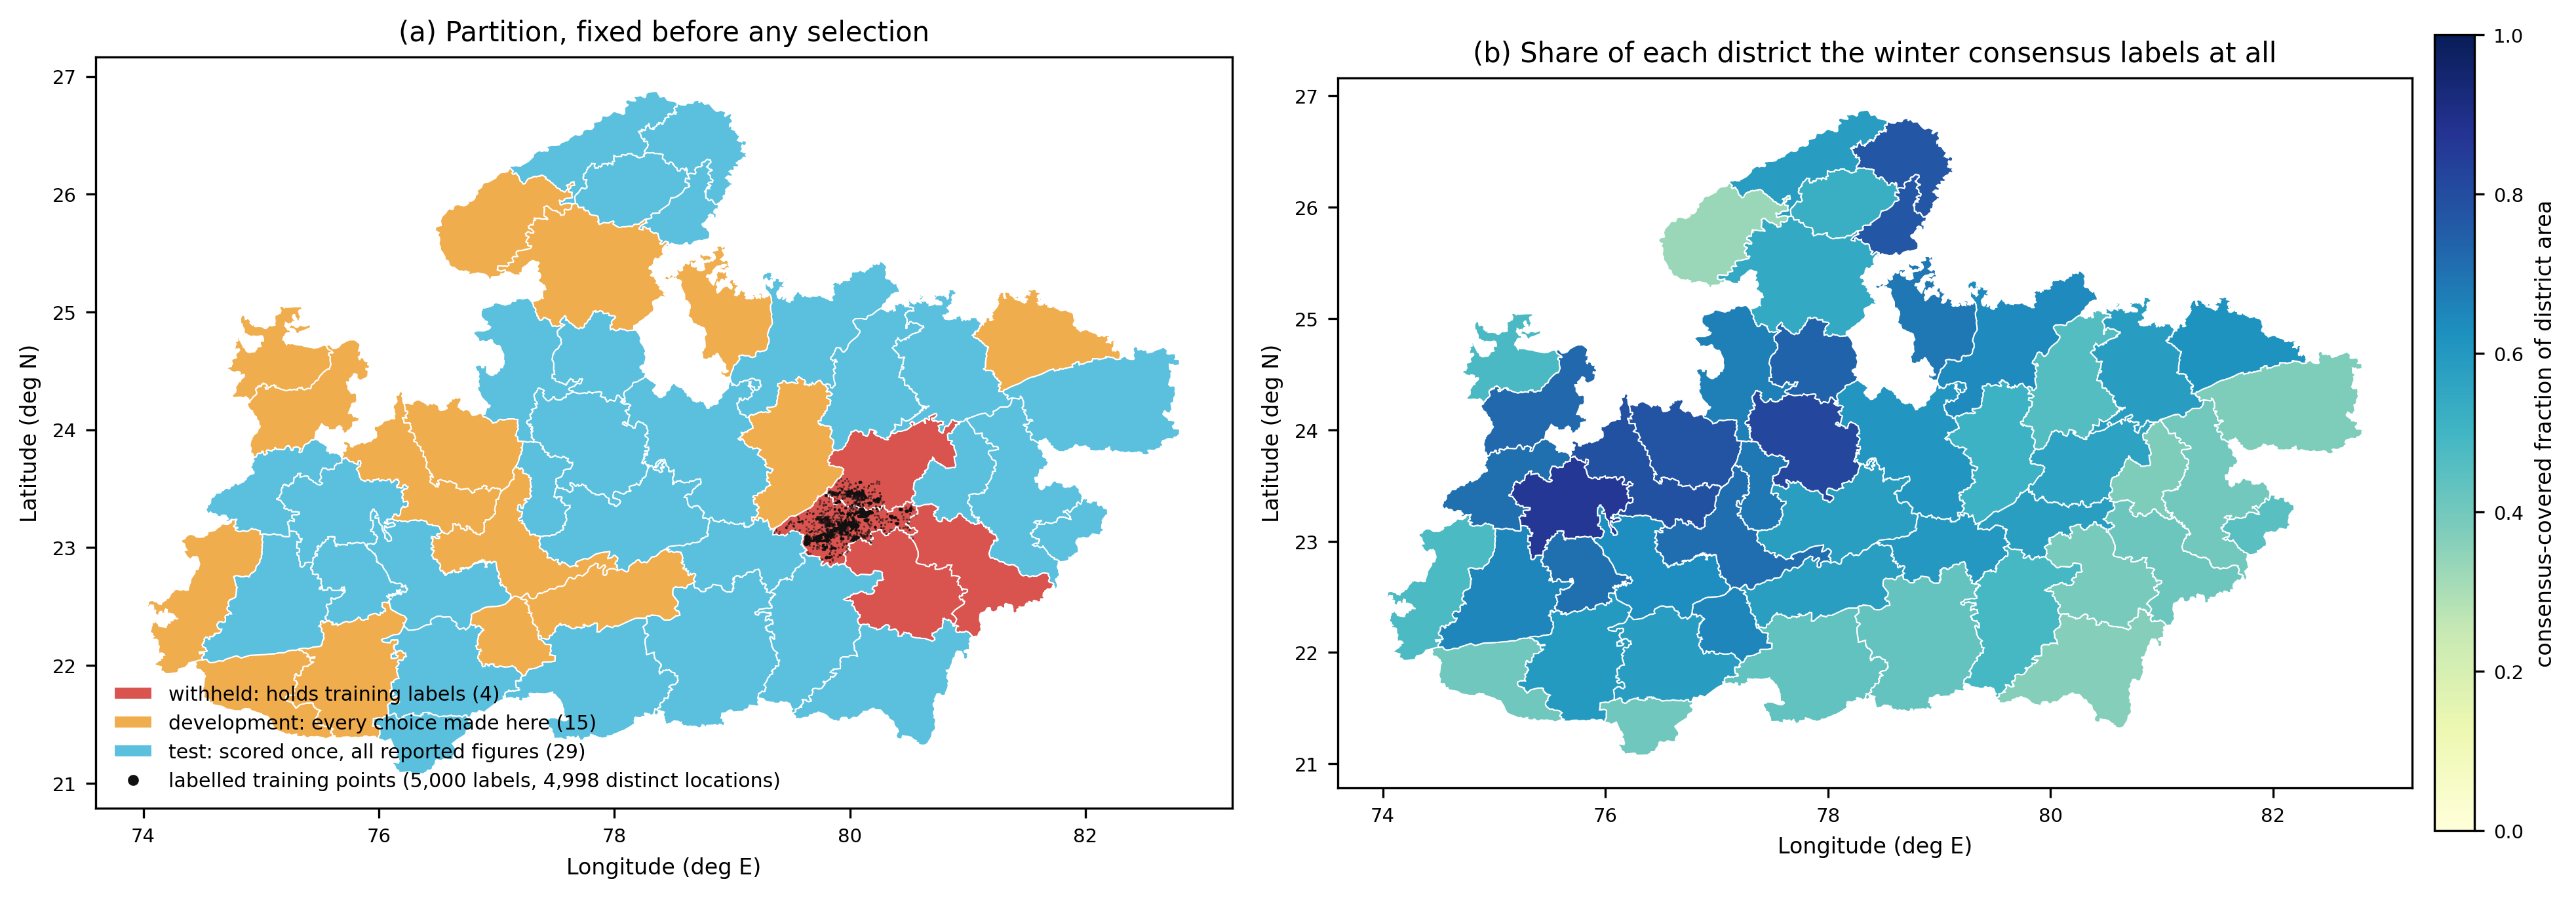
\includegraphics[width=0.95\textwidth]{fig_split_map.png}
\caption{Where the partition and the reference domain are. (a) The four withheld districts holding all 5,000 labelled points, the 15 development districts and the 29 test districts; development blocks span the state's longitude range rather than one corner. (b) The fraction of each district the winter consensus assigns to any of the five classes---the domain the area-weighted estimates of Section~\ref{sec:area} describe, its complement carrying no reported figure. Membership, blocks, sample counts and areas are in \texttt{district\_split.csv}.}
\label{fig:split_map}
\end{figure*}

\begin{table}[htbp]
\caption{Dataset and Split Manifest}
\begin{center}
\begin{tabular}{p{2.4cm}rp{3.7cm}}
\toprule
\textbf{Dataset} & \textbf{Count} & \textbf{Purpose / Notes} \\
\midrule
Jabalpur-region training & 5,000 & Model training; 1,000 per class; 100\,m buffer from every test point. Influenced model choice by construction. \\
Development, winter & 1,500 & Feature stack, classifier and hyperparameter choice; 15 districts. \\
Development, summer & 1,418 & As above; 15 districts. \\
Test, winter & 2,900 & Final winter reporting, scored once; 29 districts. No influence on any choice. \\
Test, summer & 2,692 & Final summer reporting, scored once; 29 districts. No influence on any choice. \\
Withheld districts & -- & Jabalpur, Katni, Dindori and Mandla contain labelled training points and are excluded from all reported accuracy. \\
\bottomrule
\end{tabular}
\label{tab_splits}
\end{center}
\end{table}

\FloatBarrier
\section{Results and Analysis}

\subsection{What each feature family adds}
\label{sec:families}
Table~\ref{tab_families} starts from a ten-band optical baseline and adds feature families one at a time, scored district by district on the 15 development districts against the same five-class consensus every other number in this paper uses. No new labels are added, so the gains are from features only.

\begin{table}[!htbp]
\caption{Feature-Family Attribution, Smile GTB, Selected and Scored on the 15 Development Districts Only. Each Row is the Cumulative Set Named, Not the Family Alone. ``Open R'' is Open-Land Recall and ``Built P'' Built-Area Precision.}
\label{tab_families}
\begin{center}
\setlength{\tabcolsep}{2.5pt}
\begin{tabular}{@{}llrrrr@{}}
\toprule
\textbf{Season} & \textbf{Feature set} & \textbf{Bands} & \textbf{OA} & \textbf{Open R} & \textbf{Built P} \\
\midrule
Winter & optical & 10 & 75.9\% & 42.0\% & 57.8\% \\
       & optical + bareness & 15 & 77.0\% & 40.7\% & 57.5\% \\
       & \dots + optical texture & 21 & 80.2\% & 57.3\% & 62.5\% \\
       & \dots + SAR, SAR texture & 27 & 86.7\% & 73.3\% & 73.1\% \\
\midrule
Summer & optical & 10 & 60.2\% & 32.7\% & 56.5\% \\
       & optical + bareness & 15 & 60.4\% & 30.7\% & 56.6\% \\
       & \dots + optical texture & 21 & 66.8\% & 53.7\% & 64.8\% \\
       & \dots + SAR, SAR texture & 27 & 74.8\% & 55.0\% & 72.8\% \\
\bottomrule
\end{tabular}

\vspace{2pt}
\parbox{\columnwidth}{\footnotesize Every row is a development-district figure and none is an accuracy of the method. The last row adds SAR amplitude and SAR texture together, so the table attributes their sum and not either alone; the leave-one-family-out sweep of Fig.~\ref{fig:ablation} separates them. Every figure in this table is the pooled development matrix from one stored record, \texttt{band\_ablation\_v4.json}. That sweep and the leave-one-band-out sweep were run before the hyperparameter search of Table~\ref{tab_hyper}, so the 27-band row sits 0.26 points under the same stack's tuned development accuracy in Table~\ref{tab_stacks} in winter and 0.77 points above it in summer. Comparisons within a column are unaffected, because every row is scored under one setting.}
\end{center}
\end{table}

On the development districts, the optical baseline alone reaches 75.9\% overall accuracy in winter at 42.0\% open-land recall. Adding the bareness and built-up indices moves winter open-land recall from 42.0\% to 40.7\%; adding optical texture raises it to 57.3\%, and adding SAR amplitude and SAR texture raises it further to 73.3\%. In summer the corresponding sequence is 32.7\%, 30.7\%, 53.7\% and 55.0\%. The combined feature families therefore improve discrimination substantially, but the incremental benefit of the SAR family is season dependent: 16.0 points of open-land recall in winter against 1.3 in summer. The bareness indices are the one family that does not help this confusion in either season, which is consistent with their design, since NDBI, UI and IBI were built to separate built land from vegetation rather than from dry soil \cite{r21}, \cite{r26}. These numbers quantify the predictive contribution of the tested feature sets on this reference. They are not direct measurements of individual scattering mechanisms, and the sequence is cumulative, so each row inherits everything above it. Fig.~\ref{fig:ablation} asks the same question by removal rather than by addition, which avoids crediting whichever family is added first with everything two families share: SAR amplitude is the family the stack can least afford to lose in either season, and the bareness indices are the only family whose removal ever helps.

\begin{figure*}[!t]
\centering
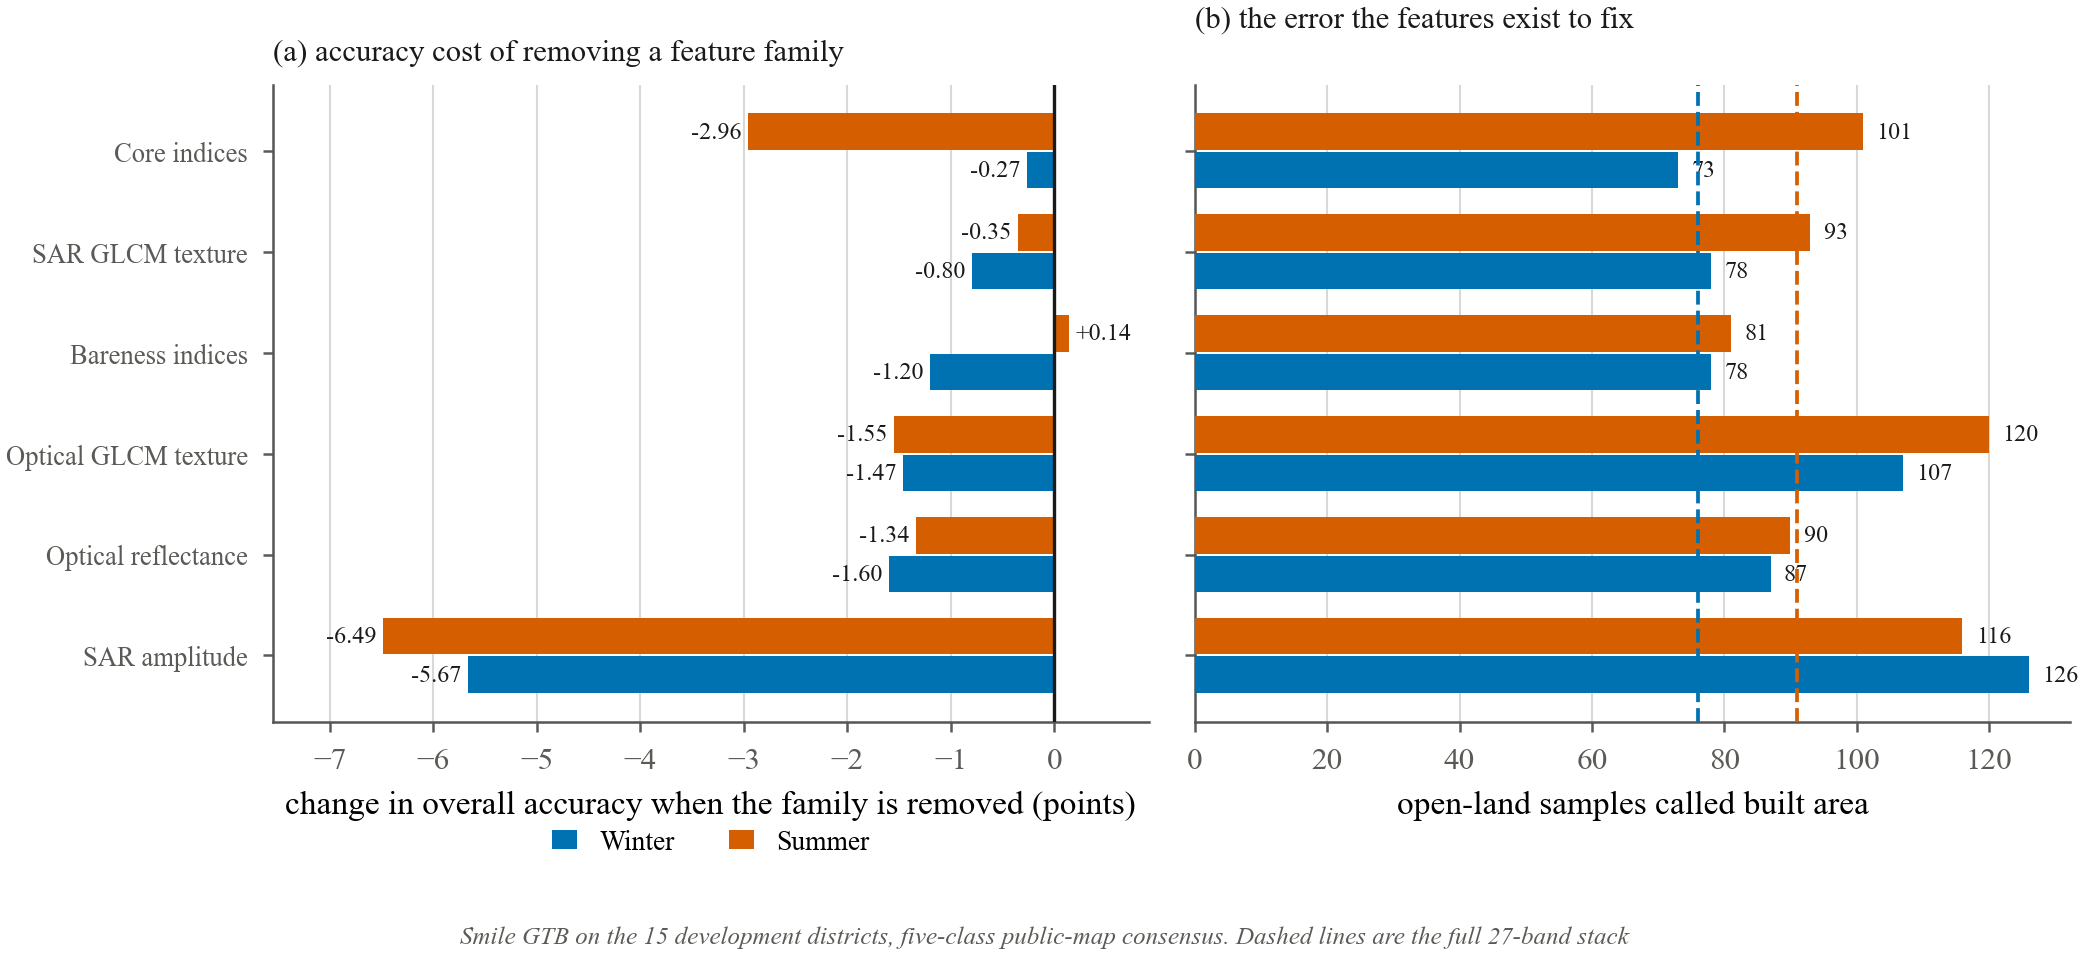
\includegraphics[width=0.92\textwidth]{fig4_feature_ablation.png}
\caption{Leave-one-family-out sweep, Smile GTB on the 15 development districts. Each bar is a change against this sweep's own 27-band baseline, 86.73\% in winter and 74.33\% in summer, so deltas are read within a panel and not against Table~\ref{tab_families}, which is a separate run. (a) Change in overall accuracy when one family is removed: SAR amplitude is the family the stack can least afford to lose in either season, and the bareness indices are the only family whose removal ever helps. (b) The error the stack exists to fix, open-land samples called built area, with dashed lines marking the full stack.}
\label{fig:ablation}
\end{figure*}

A leave-one-band-out sweep over the same districts drops the resolution from families to single bands (Fig.~\ref{fig:band_reduction}a). Its 27-band baseline is 86.67\% in winter and 74.75\% in summer, against 86.93\% and 73.98\% for the same stack in Table~\ref{tab_stacks}. The two differ because this sweep was run before the hyperparameter search of Table~\ref{tab_hyper} and that table after it; the offset is $-0.26$ points in winter and $+0.77$ in summer, so tuning is not a uniform improvement and the sign of the difference is not the same in both seasons. Both figures are recomputed from their own stored matrices in the result archive rather than copied across. The offset is constant within each experiment, so no comparison inside either is affected, but the two must not be quoted side by side as if they were one run. Against the 86.67\% baseline, the bands the stack can least afford to lose are VH (-2.60), SWIRratio (-1.53), B12 (-1.40) in winter and SWIRratio (-2.40), VH (-1.90), NDWI (-1.62) in summer, all quoted as the change in overall accuracy when that band alone is removed. Winter tolerates the loss of only two bands, summer of eight, and no single band is free to remove in both seasons at once, which is the honest answer to whether this stack carries redundant features: on a per-band test, it carries almost none.

\subsection{Reducing the feature stack from 27 bands to 19}
\label{sec:stacks}
The number of bands matters far less than which ones. A leave-one-band-out sweep nominates the bands that can go, and Table~\ref{tab_stacks} scores the stacks those nominations produce, choosing on the 15 development districts and confirming once on the 29 test districts (Fig.~\ref{fig:band_reduction}b). Every stack is trained from one sampled table carrying all 27 bands, so they differ only in which columns the classifier may read and not in which pixels survived sampling. Table~\ref{tab_stackdef} lists those columns for each candidate.

\begin{table*}[!t]
\caption{Contents of the Four Candidate Feature Stacks. Every Stack is a Subset of the Same 27 Columns of Table~\ref{tab_bands}}
\label{tab_stackdef}
\begin{center}
\setlength{\tabcolsep}{4pt}
\begin{tabular}{@{}lcL{2.3cm}L{4.3cm}L{3.7cm}L{4.0cm}@{}}
\toprule
\textbf{Stack} & \textbf{Bands} & \textbf{Reflectance} & \textbf{Spectral indices} & \textbf{Optical GLCM on B8} & \textbf{SAR amplitude; GLCM on VV} \\
\midrule
\texttt{all27} & 27 & B2, B3, B4, B8, B11, B12 & NDVI, NDWI, SAVI, NDBI, UI, IBI, SWIRratio, BSI, BAEI & contrast, variance, IDM, entropy, dissim., ASM & VV, VH, VV$-$VH; contrast, variance, entropy \\
\addlinespace[2pt]
\texttt{b22}   & 22 & B2, B3, B4, B11, B12 & SAVI, UI, IBI, SWIRratio, BSI, BAEI & contrast, variance, IDM, entropy, dissim., ASM & VV, VH, VV$-$VH; contrast, variance \\
\addlinespace[2pt]
\texttt{alt19} & 19 & B3, B11, B12 & UI, IBI, SWIRratio, BSI, BAEI & contrast, variance, IDM, entropy, dissim., ASM & VV, VH, VV$-$VH; contrast, variance \\
\addlinespace[2pt]
\texttt{sel19} & 19 & B4, B8, B11, B12 & NDVI, NDWI, SAVI, UI, IBI, SWIRratio & contrast, variance, IDM & VV, VH, VV$-$VH; contrast, variance, entropy \\
\bottomrule
\end{tabular}

\vspace{2pt}
\parbox{\textwidth}{\footnotesize \texttt{all27} is every candidate feature of Table~\ref{tab_bands}. \texttt{b22} drops B8, NDVI, NDWI, NDBI and the SAR entropy band from it. \texttt{alt19} and \texttt{sel19} are the same size and share thirteen columns: B11, B12, UI, IBI, SWIRratio, the optical GLCM measures contrast, variance and IDM, and the five SAR bands other than entropy. The remaining six are where they part: \texttt{sel19} keeps B4, B8, NDVI, NDWI, SAVI and SAR entropy, and \texttt{alt19} keeps B3, BSI, BAEI and the optical GLCM measures entropy, dissimilarity and ASM in their place. \texttt{sel19} is the stack Table~\ref{tab_bands} marks in bold and the one every accuracy figure in this paper uses.}
\end{center}
\end{table*}


The rule that produces \texttt{sel19} needs stating, because the per-band sweeps of the two seasons do not agree and neither of them alone yields nineteen bands. Winter nominates two bands as free (\texttt{g\_contrast} and the SAR entropy band) and summer nominates eight, and the two sets do not intersect. \texttt{sel19} drops the eight the summer sweep nominates and keeps the two the winter sweep nominates, because the selection rule ranks whole candidate stacks by development accuracy averaged over the two seasons rather than removing any band that a single season happens to tolerate. A stack chosen on one season's sweep alone would have hard-coded that season's phenology, as Section~\ref{sec:tuning} argues.

Two of the candidates keep exactly nineteen bands and share only thirteen of them, which makes them a controlled test of that claim. The stack labelled \texttt{sel19} keeps B4, B8, NDVI, NDWI, SAVI and the SAR entropy band; \texttt{alt19} discards all six and keeps B3, BSI, BAEI and three further optical GLCM measures instead. Ranked by development accuracy averaged over the two seasons, \texttt{sel19} leads at 81.19\% and \texttt{alt19} is last of the four at 77.99\%. Scored once on the held-out test districts, the difference between two stacks of identical size is +1.76 points in winter (95\% CI +1.00 to +2.52) and +4.91 in summer (95\% CI +3.54 to +6.42), paired by district. The stack contrasts form their own pre-specified family, three per season against the selected stack, and Holm's adjustment is applied within it as it is within the classifier family; both winter and summer differences here survive it at $p\le 0.001$.

Against the full stack, \texttt{sel19} is worth +1.93 points in winter (95\% CI +1.27 to +2.59, Holm-adjusted $p<0.001$) and +1.92 in summer (95\% CI +0.49 to +3.54, adjusted $p=0.020$), paired by district. The remaining contrast, against \texttt{b22}, is +1.66 in winter and +3.16 in summer, both adjusted $p\le0.001$; all six are in \texttt{feature\_experiments.csv} and \texttt{paired\_contrasts.csv}. What this shows is that the identity and combination of the retained features matter: the selected 19-band stack outperformed the alternative 19-band stack of the same size and the full candidate set, under the stated development rule. It does not show that a smaller feature count is intrinsically superior, and it does not isolate the relative roles of redundancy, regularisation, feature interactions and finite-sample effects, which this design cannot separate. The Hughes phenomenon \cite{r32} is the explanation usually offered for a reduction that helps, and the ordering here does not follow the pattern a simple dimensionality account would suggest, since \texttt{alt19} is the worst of the four and the full stack second. It does not follow from a dimensionality account that the largest stack must score lowest: \texttt{alt19} is not a subset of the full stack but a different selection, and removing six informative bands can cost more than carrying eight uninformative ones, so a smaller stack scoring worse than a larger one is consistent with dimensionality effects being present. The ordering therefore fails to isolate redundancy as the operative mechanism rather than ruling it out. The per-band sweep points the same way, since no single band can be dropped without measurable loss in both seasons. That is evidence against redundancy being the operative mechanism here; it is not a demonstration of what the operative mechanism is. No wall-clock saving is claimed either, since Earth Engine cost was not measured. A cut chosen on the data it is then reported against would show none of this, because it would score every candidate at its own maximum.

\begin{figure}[!htbp]
\centering
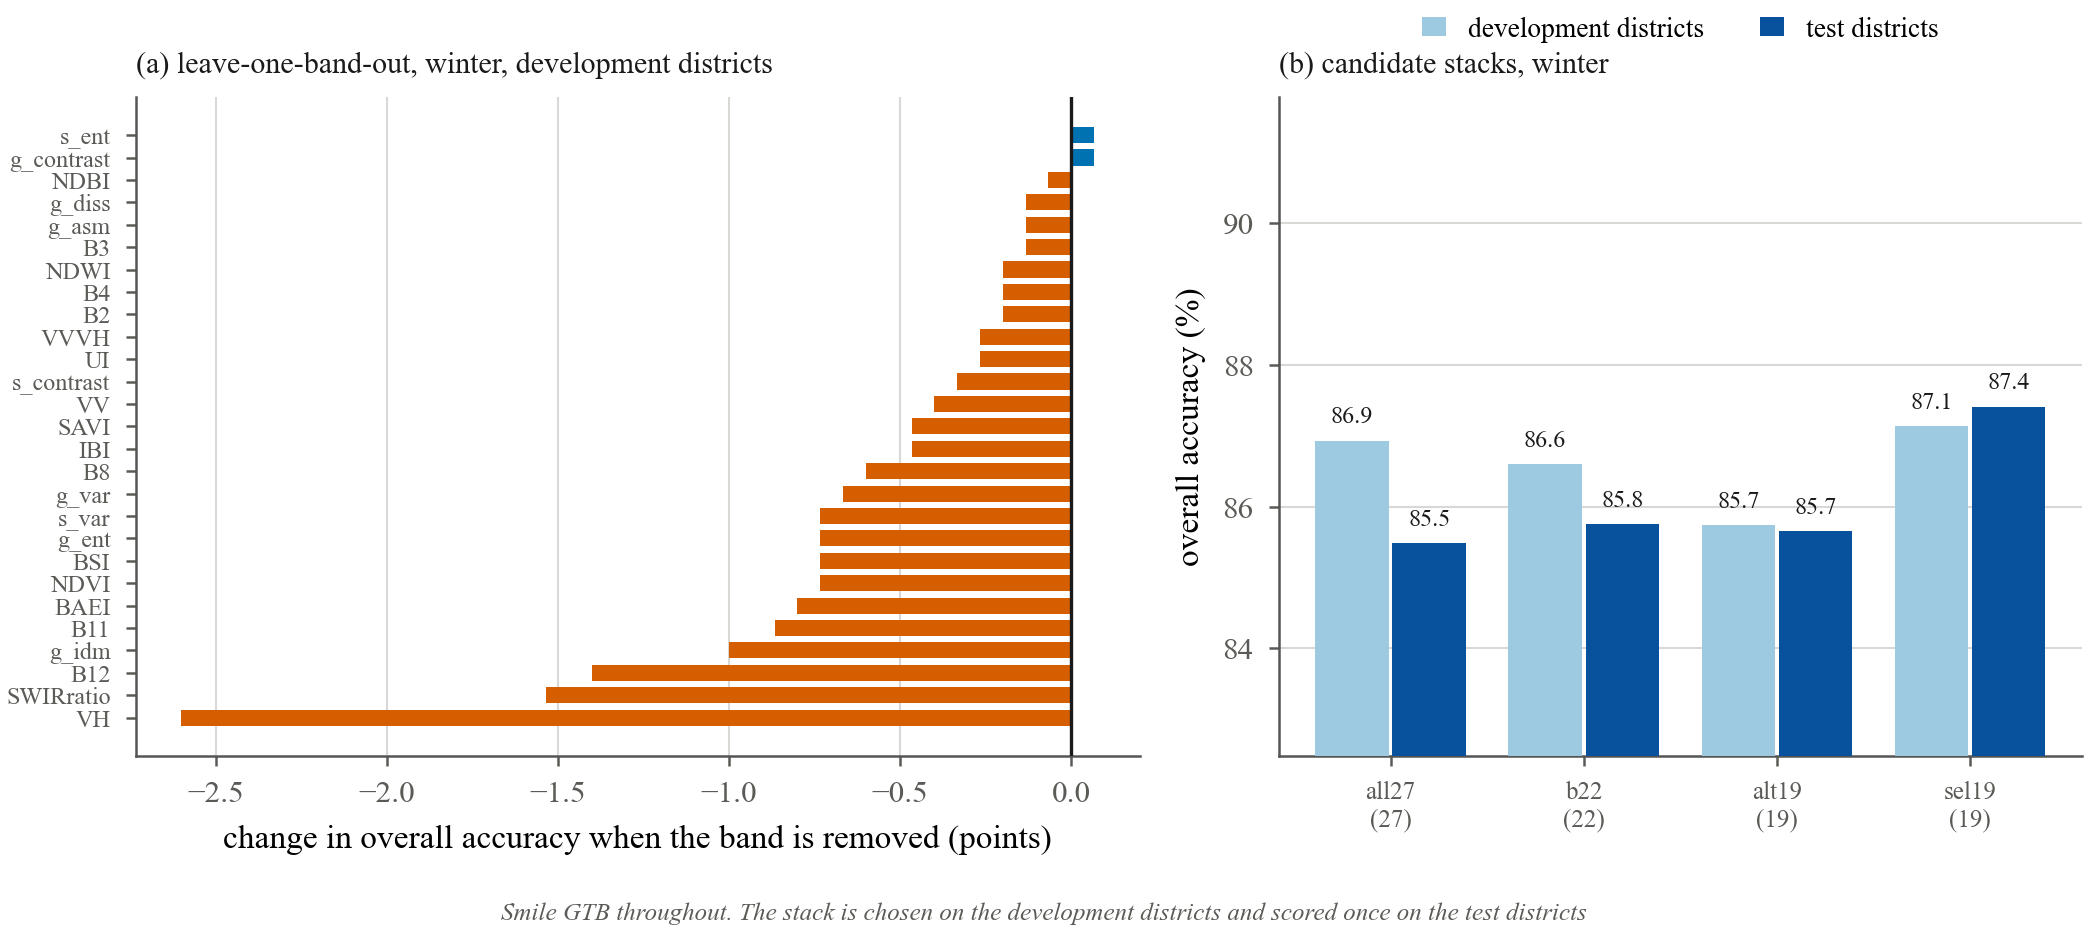
\includegraphics[width=\columnwidth]{fig10_band_reduction.png}
\caption{Choosing the feature stack, Smile GTB, winter. (a) Leave-one-band-out on the 15 development districts: only \texttt{g\_contrast} and the SAR entropy band can be removed at no winter cost, and VH is worth 2.6 points on its own. (b) The candidate stacks those removals suggest, on the development districts that chose them and the test districts that did not, with band counts in parentheses. The two 19-band stacks differ by 1.8 points on test ground despite being the same size.}
\label{fig:band_reduction}
\end{figure}

\begin{table}[!htbp]
\caption{Candidate Feature Stacks, Smile GTB. Each is Chosen on the 15 Development Districts and Scored Once on the 29 Test Districts.}
\label{tab_stacks}
\begin{center}
\setlength{\tabcolsep}{3pt}
\begin{tabular}{llrrrl}
\toprule
\textbf{Season} & \textbf{Stack} & \textbf{Bands} & \textbf{Dev.\ OA} & \textbf{Test OA} & \textbf{Test 95\% CI} \\
\midrule
Winter & \texttt{all27}  & 27 & 86.93\% & 85.48\% & [83.14, 87.90] \\
       & \texttt{b22}    & 22 & 86.60\% & 85.76\% & [83.52, 88.00] \\
       & \texttt{alt19}  & 19 & 85.73\% & 85.66\% & [83.59, 87.93] \\
       & \texttt{sel19}  & 19 & \textbf{87.13\%} & \textbf{87.41\%} & [85.07, 89.69] \\
\midrule
Summer & \texttt{all27}  & 27 & 73.98\% & 71.99\% & [69.17, 74.82] \\
       & \texttt{b22}    & 22 & 71.65\% & 70.77\% & [68.28, 73.26] \\
       & \texttt{alt19}  & 19 & 70.24\% & 68.98\% & [66.32, 71.57] \\
       & \texttt{sel19}  & 19 & \textbf{75.25\%} & \textbf{73.85\%} & [70.81, 76.82] \\
\bottomrule
\end{tabular}

\vspace{2pt}
\parbox{\columnwidth}{\footnotesize All differences quoted in the text are means of per-district differences over the 29 test districts and so do not in general equal the difference of the pooled accuracies in this table, because districts contribute unequal numbers of points; for example \texttt{sel19} minus \texttt{all27} in summer is +1.92 paired by district against +1.86 pooled. \texttt{sel19} is the selected stack of Table~\ref{tab_bands} and the one every other result in this paper uses; its rows are identical to the Smile GTB rows of Table~\ref{tab:statewide_accuracy}. The membership of all four stacks is given in Table~\ref{tab_stackdef}. Intervals resample whole districts, as in Table~\ref{tab:statewide_accuracy}.}
\end{center}
\end{table}

\subsection{Hyperparameter selection and sensitivity}
\label{sec:tuning}
A ranking built on inherited settings partly measures which model happened to inherit a workable configuration rather than which model is better. A grid of 28 configurations in total across the five models (Table~\ref{tab_hyper}: six for Random Forest, six for SVM, eight for Smile GTB, four for CART and four for KNN) was therefore run per season on the 15 development districts, and only there, so that the selected configuration could afterwards be scored once on the test districts and still be an estimate rather than a maximum over a search. Table~\ref{tab_hyper} gives the grid and what it chose. How much this matters differs sharply by model. Across the winter grid, development accuracy spans 4.7 points for Random Forest and 3.3 for SVM, but only 1.3 for Smile GTB and about half a point for KNN and CART; in summer Random Forest spans 9.5 points. The two models most sensitive to their settings are therefore the two that an untuned comparison would misrepresent worst. Tuning narrowed the spread between models on the development districts; whether it would have changed the order at the top cannot be told from this design, because the untuned pipeline was never scored on the test districts and doing so afterwards would have spent the held-out half twice. Winter and summer do not always agree on a configuration---summer prefers a shallower, more heavily shrunk booster and a wider SVM kernel---and one configuration per model, the winter choice, is used in both seasons and in the dashboard, so that a single deployed model is being reported rather than a per-season best.

The two seasons do not agree on which bands to drop, and the disagreement is informative rather than noise. The two disjoint nomination sets are those of Section~\ref{sec:stacks}: winter spares two bands and summer eight, with no overlap, so no band is safely droppable in both. The reason is phenological. In summer the cultivated fields that dominate the state are bare, so the bareness indices carry little class information and can go; in winter they are green, and the same indices are doing work. Selecting on one season alone would therefore have hard-coded that season's phenology into the stack, and the rule used here instead ranks stacks by development accuracy averaged over the two seasons the paper reports.

\subsection{Classifier comparison over 29 held-out test districts}
\label{sec:models}
Table~\ref{tab:statewide_accuracy} reports all five models on the public-map consensus over the 29 test districts (2,900 winter and 2,692 summer samples). The ranking itself was decided on the development districts; these numbers are the consequence of that decision rather than its basis.

\begin{table}[!htbp]
\caption{External Agreement over the 29 Held-Out Test Districts (2,900 Winter and 2,692 Summer Reference Samples), Pooled over Districts}
\label{tab:statewide_accuracy}
\centering
\setlength{\tabcolsep}{3.5pt}
\begin{tabular}{llrlr}
\toprule
\textbf{Season} & \textbf{Model} & \textbf{OA} & \textbf{95\% CI\textsuperscript{*}} & \textbf{Kappa} \\
\midrule
Winter & Smile GTB & 87.41\% & [85.07, 89.69] & 0.843 \\
       & RF        & 86.45\% & [84.17, 88.59] & 0.831 \\
       & SVM (RBF) & 86.38\% & [84.03, 88.59] & 0.830 \\
       & KNN       & 85.28\% & [83.17, 87.55] & 0.816 \\
       & CART      & 80.55\% & [78.28, 82.86] & 0.757 \\
\midrule
Summer & Smile GTB & 73.85\% & [70.81, 76.82] & 0.669 \\
       & RF        & 71.84\% & [68.43, 75.23] & 0.643 \\
       & KNN       & 69.65\% & [66.33, 72.99] & 0.616 \\
       & SVM (RBF) & 68.61\% & [65.87, 71.36] & 0.602 \\
       & CART      & 61.33\% & [58.58, 63.98] & 0.509 \\
\bottomrule
\end{tabular}

\vspace{2pt}
\parbox{\columnwidth}{\textsuperscript{*}\footnotesize Percentile interval over 5,000 bootstrap replicates that resample whole districts, not points. Samples inside one district share landscape, phenology and reference-map error, so a pixel-level interval would be far too narrow. Every value is a pooled count over the 29 districts, run identifiers \texttt{v7-\{season\}-test-after-\{model\}} in \texttt{metrics.csv}; the paired comparisons of Table~\ref{tab_paired} are means of per-district differences instead, and the two aggregations do not in general agree, because districts contribute unequal numbers of points.}
\end{table}

\begin{figure}[!htbp]
\centering
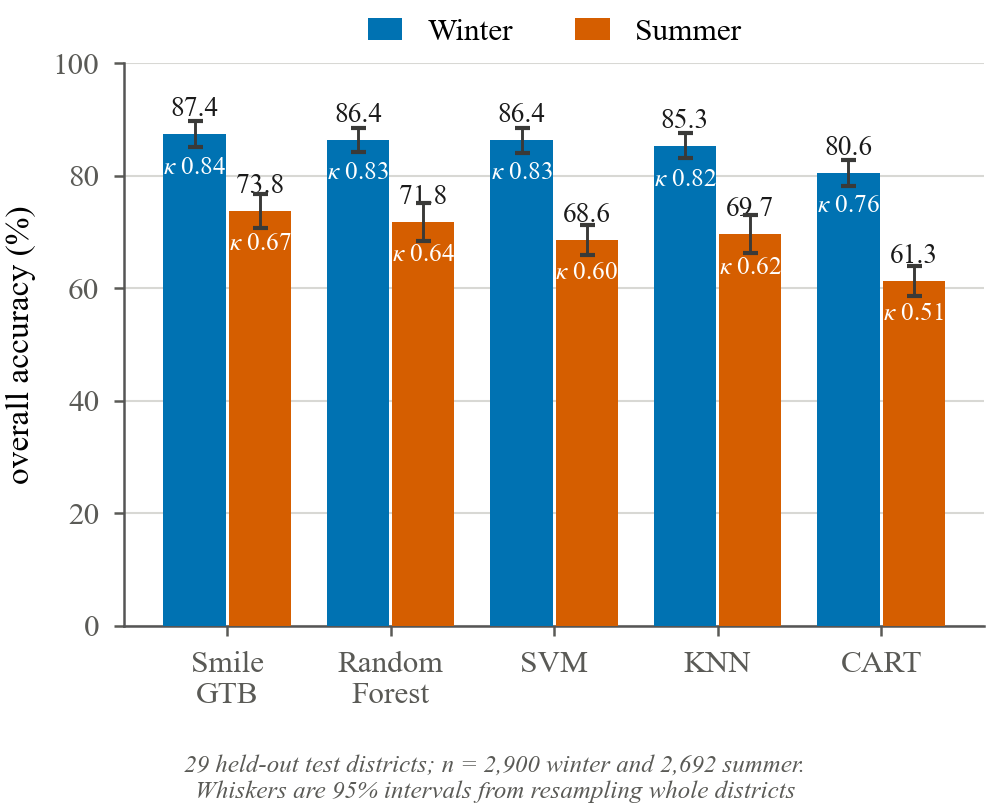
\includegraphics[width=\columnwidth]{fig5_statewide_accuracy.png}
\caption{External accuracy of the five classifiers over the 29 held-out test districts in both seasons, with the Kappa coefficient inset in each bar. Whiskers are 95\% intervals from resampling whole districts; they overlap for the top three classifiers in winter.}
\label{fig:statewide_acc}
\end{figure}

Smile GTB has the highest point estimate in both seasonal test summaries: 87.41\% OA and Kappa 0.843 in winter, 73.85\% and 0.669 in summer (Fig.~\ref{fig:statewide_acc}). These are unweighted accuracies over a sample that takes up to 20 points per class per district and so treats the five classes as roughly equally common, which they are not on the ground. The quota is met exactly in winter and misses only in summer vegetation, so the winter sample is exactly balanced and the summer one is 580 points in four classes against 372 in the fifth. Weighting each stratum by its share of the reference domain gives 75.50\% $\pm$ 3.32 points in winter and 58.67\% $\pm$ 4.01 in summer (Table~\ref{tab_coverage}); the gap between the two pairs of numbers is a property of the sampling design rather than a disagreement about the maps, and Section~\ref{sec:area} sets out what each estimates. The unweighted figures are the ones used for every comparison below, because every comparison is between models scored on the same sample.

Table~\ref{tab_paired} gives the complete set of paired comparisons against the leading model: four contrasts per season, each on the same 29 district identifiers, each with the mean per-district difference, a percentile interval from resampling those identifiers jointly for both models, and the signed-rank $p$ adjusted for multiplicity. The multiplicity family is declared as one season, four contrasts, and that choice is held for both seasons rather than selected after the fact; Holm's step-down procedure \cite{r34} is applied within it. The signed-rank test is reported as a sensitivity analysis alongside the interval, not as the primary quantity: its target is the distribution of signs and ranks, whereas the effect of interest is the mean district difference, so both are given with their disagreements intact.

The winter result is that the leading model is not separated from the two closest comparators. Against SVM the mean per-district difference is +1.03 points with a bootstrap interval of +0.03 to +2.07 that excludes zero, while the signed-rank test on the same 29 districts gives a raw $p=0.062$ and a Holm-adjusted $p=0.125$; against Random Forest the difference is +0.97 points, interval $-0.00$ to +1.97, raw $p=0.103$, adjusted $p=0.125$. The interval and the test disagree because one is a percentile interval on a mean of district differences and the other is a rank test on their signs, and the more conservative reading is the one carried into the abstract and the conclusion. The remaining two winter contrasts do survive adjustment, against KNN (+2.14, adjusted $p=0.003$) and CART (+6.86, adjusted $p<0.001$). In summer all four contrasts survive, the largest adjusted $p$ being 0.019 against Random Forest.

Table~\ref{tab_paired} tests four contrasts, all of them against the leading model, which is the family declared before the test districts were scored. Two statements in this paper are about pairs that family does not contain: that CART is separated from every other classifier, and that the remaining models form a group. Those need the other six contrasts, so Table~\ref{tab_pairwise_all} reports all ten unordered pairs per season under the same procedure, with Holm applied within the larger family of ten. The two tables therefore give different adjusted $p$ for the same raw $p$, and each says which family it used; the four-contrast table remains the pre-specified one and the ten-contrast table is a secondary analysis reported because the claims above require it.

It supports the CART statement and weakens one other. CART is separated from all four other classifiers in both seasons, every adjusted $p$ below 0.001, so that claim survives being tested rather than asserted. Against that, Random Forest and SVM are indistinguishable in winter (+0.07 points, adjusted $p=0.96$), and the summer margin of the leading model over Random Forest, which the pre-specified family reports as adjusted $p=0.019$, does not survive adjustment within the family of ten ($p=0.061$). A reader who wants one classifier declared best in summer should note that the answer depends on how many comparisons are being counted.

The conclusion that follows is a negative one and is stated as such. Smile GTB has the highest point estimate in both seasons. The reported winter differences from SVM and Random Forest are small and are not consistently distinguished by the available inference procedures. This study therefore does not establish a unique best winter classifier, and it equally does not establish statistical equivalence among the leading models: a non-significant paired test on 29 districts is not evidence that two classifiers perform the same, and no equivalence bound was specified or tested. CART is the one model separated from every other in both seasons, and KNN sits between the two groups.

\begin{table}[!htbp]
\caption{All Ten Pairwise Classifier Contrasts, Same 29 Test Districts, Holm-Adjusted within the Family of Ten}
\label{tab_pairwise_all}
\begin{center}
\setlength{\tabcolsep}{2pt}
\footnotesize
\begin{tabular}{@{}llrlrr@{}}
\toprule
\textbf{Season} & \textbf{Contrast} & \textbf{Diff.} & \textbf{95\% CI} & \textbf{Raw $p$} & \textbf{Holm $p$} \\
\midrule
Winter & GTB $-$ RF   & +0.97 & [$-$0.00, +1.97] & 0.103 & 0.250 \\
       & GTB $-$ SVM  & +1.03 & [+0.03, +2.07]   & 0.062 & 0.250 \\
       & GTB $-$ KNN  & +2.14 & [+1.10, +3.17]   & 0.001 & 0.006 \\
       & GTB $-$ CART & +6.86 & [+5.52, +8.28]   & $<$0.001 & $<$0.001 \\
       & RF $-$ SVM   & +0.07 & [$-$1.07, +1.24] & 0.964 & 0.964 \\
       & RF $-$ KNN   & +1.17 & [+0.31, +2.14]   & 0.037 & 0.187 \\
       & RF $-$ CART  & +5.90 & [+4.69, +7.17]   & $<$0.001 & $<$0.001 \\
       & SVM $-$ KNN  & +1.10 & [+0.07, +2.14]   & 0.083 & 0.250 \\
       & SVM $-$ CART & +5.83 & [+4.90, +6.83]   & $<$0.001 & $<$0.001 \\
       & KNN $-$ CART & +4.72 & [+3.72, +5.76]   & $<$0.001 & $<$0.001 \\
\midrule
Summer & GTB $-$ RF   & +1.97 & [+0.52, +3.55]   & 0.019 & 0.061 \\
       & GTB $-$ SVM  & +5.25 & [+3.03, +7.56]   & $<$0.001 & 0.002 \\
       & GTB $-$ KNN  & +4.22 & [+2.17, +6.29]   & $<$0.001 & 0.004 \\
       & GTB $-$ CART & +12.46 & [+10.4, +14.5]  & $<$0.001 & $<$0.001 \\
       & RF $-$ SVM   & +3.29 & [+1.02, +5.59]   & 0.015 & 0.061 \\
       & RF $-$ KNN   & +2.26 & [+0.55, +3.99]   & 0.035 & 0.071 \\
       & RF $-$ CART  & +10.49 & [+8.39, +12.77] & $<$0.001 & $<$0.001 \\
       & SVM $-$ KNN  & $-$1.03 & [$-$2.94, +0.80] & 0.387 & 0.387 \\
       & SVM $-$ CART & +7.20 & [+5.54, +8.90]   & $<$0.001 & $<$0.001 \\
       & KNN $-$ CART & +8.23 & [+6.00, +10.62]  & $<$0.001 & $<$0.001 \\
\bottomrule
\end{tabular}

\vspace{2pt}
\parbox{\columnwidth}{\footnotesize Procedure, seed and interval as in Table~\ref{tab_paired}; only the multiplicity family differs, being all ten pairs of a season rather than the four against the leader. Computed by \texttt{scripts/all\_pairwise\_contrasts.py} from \texttt{district\_confusion\_matrices.csv} and stored in \texttt{pairwise\_contrasts\_all.csv}.}
\end{center}
\end{table}

\begin{table}[!htbp]
\caption{Every Paired Contrast against the Leading Model, over the Same 29 Test Districts}
\label{tab_paired}
\begin{center}
\setlength{\tabcolsep}{2pt}
\footnotesize
\begin{tabular}{@{}llrlrr@{}}
\toprule
\textbf{Season} & \textbf{Contrast} & \textbf{Diff.} & \textbf{95\% CI} & \textbf{Raw $p$} & \textbf{Holm $p$} \\
\midrule
Winter & GTB $-$ RF   & +0.97 & [$-$0.00, +1.97] & 0.103 & 0.125 \\
       & GTB $-$ SVM  & +1.03 & [+0.03, +2.07]   & 0.062 & 0.125 \\
       & GTB $-$ KNN  & +2.14 & [+1.10, +3.17]   & 0.001 & 0.003 \\
       & GTB $-$ CART & +6.86 & [+5.52, +8.28]   & $<$0.001 & $<$0.001 \\
\midrule
Summer & GTB $-$ RF   & +1.97 & [+0.52, +3.55]   & 0.019 & 0.019 \\
       & GTB $-$ SVM  & +5.25 & [+3.03, +7.56]   & $<$0.001 & 0.001 \\
       & GTB $-$ KNN  & +4.22 & [+2.17, +6.29]   & 0.001 & 0.002 \\
       & GTB $-$ CART & +12.46 & [+10.4, +14.5] & $<$0.001 & $<$0.001 \\
\bottomrule
\end{tabular}

\vspace{2pt}
\parbox{\columnwidth}{\footnotesize Differences are means of per-district overall-accuracy differences, in percentage points. Intervals are percentile intervals over 5,000 replicates that resample the 29 district identifiers once and apply the same resample to both models, with seed 20260901, so the interval is on the paired effect. $p$ values are two-sided Wilcoxon signed-rank on the 29 district differences, with zero differences dropped; in winter 7 districts tie against RF, 4 against SVM, 1 against KNN and none against CART, and in summer 7, 3, 1 and none. Tied absolute differences are present in every contrast, so SciPy's asymptotic normal approximation is used throughout rather than the exact permutation distribution. Holm's step-down adjustment is applied within each season, treating that season's four contrasts as one family. Non-significance is not equivalence: no equivalence margin is specified or tested anywhere in this paper.}
\end{center}
\end{table}

Independently of any of that, there is a floor on how sharply this evidence can separate two classifiers, and it has to be measured rather than inferred. Two quantities are involved and the paper keeps them apart. The intervals of Table~\ref{tab:statewide_accuracy} and the paired intervals of Table~\ref{tab_paired} are district sampling uncertainty: they say how much the answer depends on which districts were drawn, conditional on the fitted models. They say nothing at all about how much the fitted models themselves move, because every replicate resamples the same stored predictions. That second quantity is fitting variability, and it is reported here separately.

Two records bear on it. The first is a rebuild of the whole evaluation months later---the same seeded reference sample, reclassified---which does not reproduce the stored run exactly. The difference is published in \texttt{reproduction\_check.csv} as a matrix redistribution statistic $D$, defined at Eq.~\eqref{eq:matrixdist}: 531 for Smile GTB against 1 each for Random Forest, SVM, KNN and CART, all four in the same district. $D$ is a lower bound on the number of changed point predictions and not a count of them, and the frozen run stored confusion matrices rather than per-point predictions, so the exact pointwise figure cannot be recovered from that comparison. What that rebuild changed was everything at once: the image request, the consensus construction, the stratified sample, the feature table and the fit.

The second record isolates the fit, and it contradicts the reading the rebuild invited. The evaluation table was sampled once at the 2{,}900 stored test locations and held fixed; the training table was then supplied to four successive fits of each classifier in three ways, and every fit was compared with the others prediction by prediction rather than by its pooled score alone.

Given the same training table, the fit is exactly reproducible. In all three modes, and for all five classifiers, four repeats returned the same pooled agreement to three decimal places and not one of the 2{,}900 point predictions changed. There is no unseeded generator inside these classifiers.

Sampling the training table freshly from Earth Engine before each fit also reproduces exactly, and reproduces the frozen run: Smile GTB returns 87.414\% four times, which is the stored figure of Table~\ref{tab:statewide_accuracy} to every digit the archive holds, and SVM likewise returns 86.379\%. Random Forest, KNN and CART differ from their stored figures by one or two reference points out of 2{,}900. On this comparison the model the earlier rebuild singled out as unstable is one of the two that reproduce exactly, which is the clearest evidence that the rebuild's $D=531$ was not a property of the classifier.

What does move the fit is a change to the training table that ought to be immaterial. Permuting the order of the 5{,}000 rows, changing no value, moves pooled agreement over a range of 0.38 points for Smile GTB and Random Forest, 0.76 for SVM and 0.03 for CART, and leaves KNN untouched as a lazy learner should be; 119, 79, 26 and 8 individual predictions change. Merely round-tripping the same table through a client-side representation, which alters nothing but the way the numbers are transported, moves Smile GTB from 87.414\% to 87.241\%. Those displacements are the size of the winter margins the ranking rests on, $+1.03$ over SVM and $+0.97$ over Random Forest.

The correct statement is therefore narrower and firmer than the one this paper previously made. The classifiers are deterministic; the fit is a sensitive function of a training table whose exact composition, order and numeric representation nothing in this workflow pins across sessions; and the size of that sensitivity is comparable to the differences being used to rank models. \texttt{refit\_variability.json} carries every fit and every changed-prediction count.

The band rescaling of Section~\ref{sec:features} is what makes that ranking meaningful at all. Measured on a benchmark that pools the 15 development and 29 test districts, and so is reported here only for this preprocessing comparison, the two distance-based classifiers scored 71.34\% (SVM) and 73.68\% (KNN) in winter when GLCM variance entered on its raw scale, placing them last. Mapping every band onto a common $[0, 1]$ range moves SVM by 12.76 percentage points and KNN by 9.48 on that same benchmark, and lifts both into the group they occupy here. The effect is a property of the preprocessing, not of the classifiers: the tree-based models, which split on one feature at a time, barely move.

Comparing five classifiers on one reference set and then reporting the winner's score from that same set makes the reported figure a maximum over five choices rather than an estimate of skill. The design here avoids that. The districts are partitioned once, by spatial block and before anything is selected, into 15 development and 29 test districts, with the four districts that hold training points withheld from both. Model settings, candidate feature stacks and the planned comparisons were fixed before the final evaluation records were examined; the test half was then used to estimate performance and to report those pre-specified contrasts, and was not used to choose a new configuration. Reporting several frozen models on that set, as Table~\ref{tab:statewide_accuracy} does, does not mechanically spend it: what would spend it is letting a test outcome determine a further choice, and no choice in this paper was made that way. Any analysis influenced by earlier access to the same records is identified as exploratory, which here means the distance regression of Section~\ref{sec:spatial}. The analysis chronology and the split manifest accompany the archive.

Two honest qualifications go with that. Earlier statewide evaluations were run before this partition existed, on a population that included what are now test districts; they informed the decision to partition at all, contributed no feature, model or hyperparameter choice, and none of their numbers appears in this paper. And the family-ablation and leave-one-band-out experiments of Section~\ref{sec:families} were run before the hyperparameter search of Table~\ref{tab_hyper} and therefore under the pre-search settings, which is the source of the 0.26-point winter and 0.77-point summer offsets recorded in Section~\ref{sec:families}. That offset does not apply between Table~\ref{tab_stacks} and Table~\ref{tab:statewide_accuracy}: both report the frozen post-search pipeline, and the \texttt{sel19} test entries of the first are identical to the Smile GTB entries of the second at 87.41\% and 73.85\%.

\subsection{Per-class scores}
Table~\ref{tab_f1} and Fig.~\ref{fig:per_class_f1} list per-class F1. Water is the easiest class for every classifier in both seasons, and agriculture the hardest, but the ordering of the middle three is not constant: it changes with the season. For Smile GTB in winter the order is water (0.981), vegetation (0.934), built area (0.856), open land (0.800), agriculture (0.790). In summer it is water (0.919), built area (0.854), open land (0.633), vegetation (0.594), agriculture (0.572). Vegetation moves from second place to fourth, and the size of the move is the single largest per-class change between the seasons: its recall falls from 91.03\% to 44.09\%, a drop of 46.9 points, against 16.7 points for open land and 15.2 for agriculture. Any account of the seasonal gap that centres on the built-area and open-land pair, as the design rationale of this paper does, therefore describes winter and not summer. Fig.~\ref{fig:confusion_matrices} shows where the residual error goes for the leading model, row-normalised so each row is read as the fate of one reference class.

\begin{table}[!htbp]
\caption{Per-Class F1 over the 29 Held-Out Test Districts, Pooled over Districts. Run Identifiers \texttt{v7-\{season\}-test-after-\{model\}} in \texttt{metrics.csv}}
\label{tab_f1}
\begin{center}
\setlength{\tabcolsep}{3.5pt}
\begin{tabular}{@{}llrrrrr@{}}
\toprule
\textbf{Season} & \textbf{Model} & \textbf{Veg.} & \textbf{Water} & \textbf{Built} & \textbf{Open} & \textbf{Agri.} \\
\midrule
Winter & Smile GTB     & 0.934 & 0.981 & 0.856 & 0.800 & 0.790 \\
       & Random Forest & 0.907 & 0.973 & 0.855 & 0.802 & 0.778 \\
       & KNN           & 0.928 & 0.971 & 0.824 & 0.753 & 0.772 \\
       & CART          & 0.829 & 0.954 & 0.819 & 0.729 & 0.675 \\
       & SVM           & 0.940 & 0.977 & 0.836 & 0.753 & 0.802 \\
\midrule
Summer & Smile GTB     & 0.594 & 0.919 & 0.854 & 0.633 & 0.572 \\
       & Random Forest & 0.515 & 0.896 & 0.850 & 0.643 & 0.521 \\
       & KNN           & 0.510 & 0.958 & 0.823 & 0.600 & 0.452 \\
       & CART          & 0.335 & 0.854 & 0.728 & 0.495 & 0.342 \\
       & SVM           & 0.377 & 0.956 & 0.835 & 0.589 & 0.458 \\
\bottomrule
\end{tabular}
\end{center}
\end{table}

\begin{figure*}[!t]
\centering
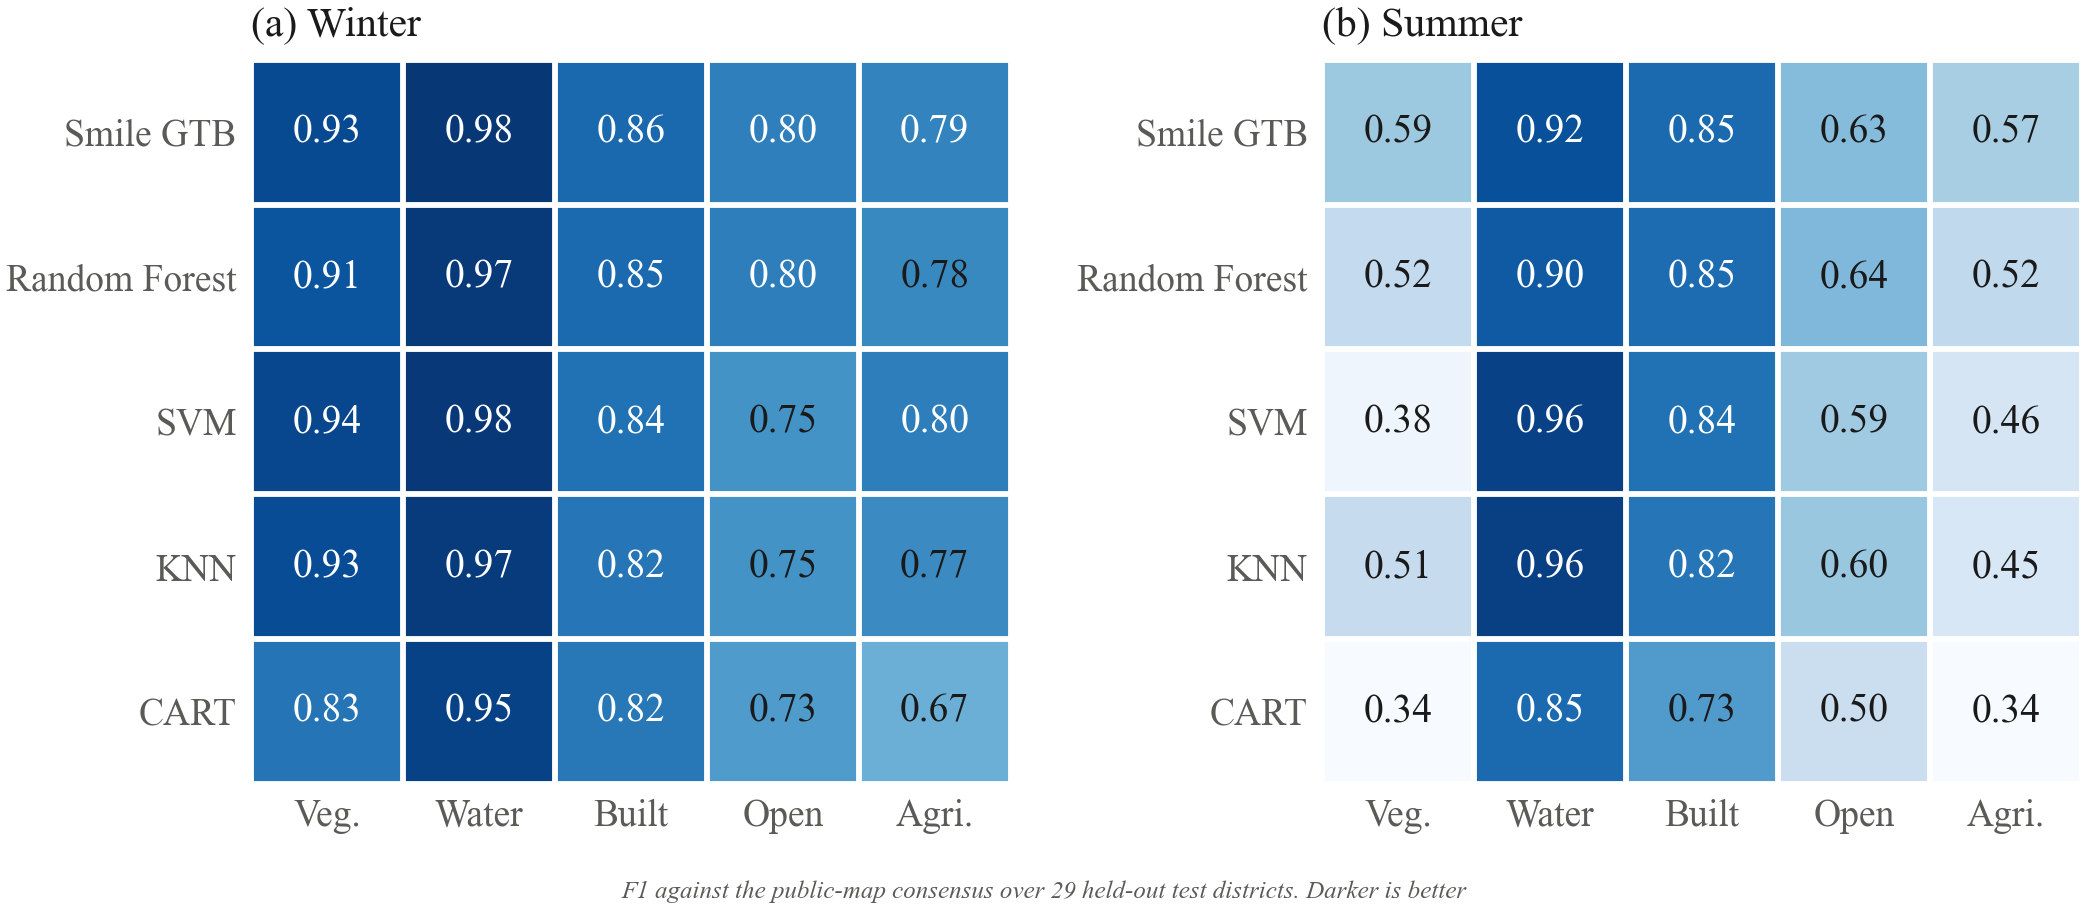
\includegraphics[width=0.95\textwidth]{fig6.png}
\caption{Per-class F1 for every classifier against the public-map consensus over the 29 held-out test districts. (a) Winter. (b) Summer. The class order is stable across classifiers, and the winter-to-summer fall is concentrated in vegetation and agriculture, the two classes that exchange members with the season.}
\label{fig:per_class_f1}
\end{figure*}

\begin{figure*}[!t]
\centering
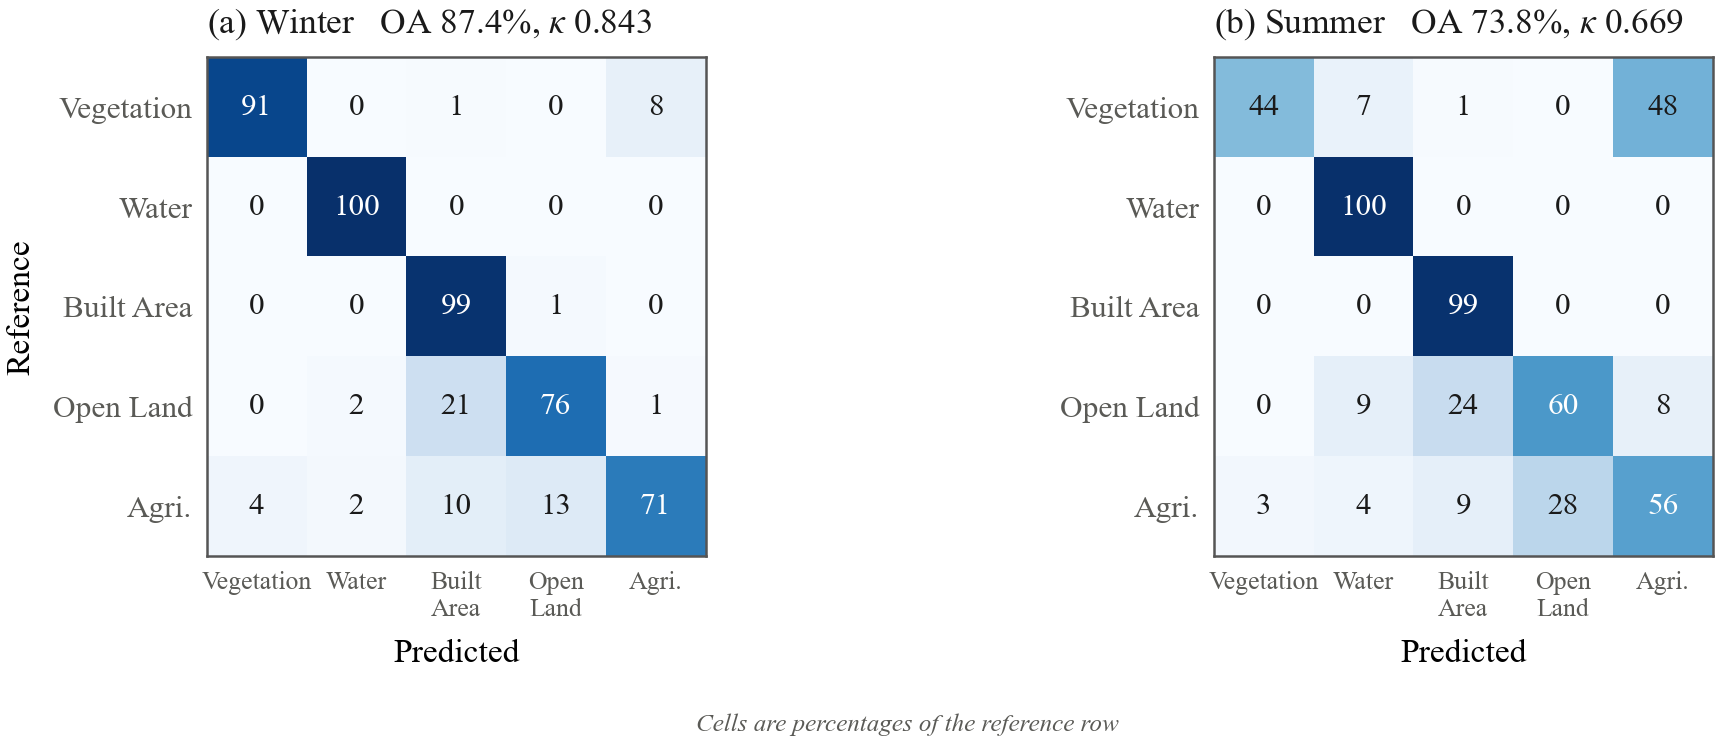
\includegraphics[width=0.95\textwidth]{fig7.png}
\caption{Smile GTB confusion matrices over the 29 held-out test districts, row-normalised to the reference row. (a) Winter, OA 87.4\%, $\kappa=0.843$: the open-land and agriculture rows carry 305 of 365 errors, and 21\% of open land is called built area. (b) Summer, OA 73.8\%, $\kappa=0.669$: the largest single confusion is vegetation into agriculture (48.4\% of the vegetation row), not open land into built area, so the error the feature stack was designed against is not the dominant summer error.}
\label{fig:confusion_matrices}
\end{figure*}

The summer vegetation failure deserves its own statement, because it is the largest error in the paper and it is not the error the feature stack was designed against. Of the 372 summer vegetation reference points, 180 are classified as agriculture and only 164 as vegetation. Three things hold at once and this design cannot separate them. The reference itself nearly vanishes for this class in summer, from 2,039\,km$^2$ of eligible area to 121\,km$^2$, so the 372 surviving points are whatever the consensus still accepted rather than a representative sample of the state's woody vegetation; deciduous canopy over central India is at its most senescent in the April--May window, so the spectral distinction from a bare or stubbled field is genuinely weakest then; and the training labels for this class were interpreted on a winter composite in four districts. Which of the three dominates is not measured here. What can be said is that the surviving 0.12\% of eligible area is a residue selected by the consensus rule, so the 44.09\% recall is an agreement figure over that residue and should not be read as a summer vegetation accuracy for Madhya Pradesh.

\subsection{What the two seasons actually rest on}
\label{sec:seasonal_support}
Matched windows and matched granule counts are scene-level statements. Two per-pixel quantities decide whether they support the interpretation usually put on them, and both were measured on four test districts spanning the state (Anuppur, Chhatarpur, Gwalior and Sagar), at 300\,m over the whole district.

The first is observation depth. Counting Sentinel-2 observations that survive both the scene-level cloud filter and the QA60 mask, the district means run 14.9 to 22.4 in winter and 13.7 to 17.4 in summer, averaging 17.5 against 15.4, and the fifth percentile of the per-pixel count falls from 7--10 in winter to 7--9 in summer. Summer therefore rests on about 12\% fewer usable optical observations per pixel than winter, a difference the matched granule counts of Section~\ref{sec:seasons} do not show, because a granule intersecting a district is not an observation of a pixel. Sentinel-1 depth is identical between seasons in every district audited, 5.0 to 6.9 scenes, as the orbit geometry implies.

The second is clipping. The scaling bounds of Table~\ref{tab_scales} are fitted on winter and applied to summer, so the obvious worry is that summer values run past a winter tail and are tied together. Measured, the asymmetry runs the other way. The most clipped band is optical GLCM contrast, and it is clipped in 7.3\% of winter pixels against 1.7\% of summer pixels; SAR contrast is clipped in 2.7\% against 2.0\%; every other rescaled band clips under 1\% in both seasons, and SWIRratio never reaches its bound. Winter, the season the bounds were fitted on, is the season that saturates more, which is consistent with the bounds being 99th percentiles of a winter sample rather than maxima. Shared scaling is thus not supported as a mechanism by this audit, which is a weaker statement than ruling it out and is the one the measurement licenses. The rates above are district-wide aggregates at 300\,m over four of the 29 test districts, pooled across all land covers. A clipping rate that is low overall can still be high within one class, and it is the class-conditional rate that would matter for a class-specific accuracy drop; that quantity was not measured, and neither was any interaction between clipping and the distance-based classifiers. The audit shows that the obvious form of the scaling worry does not appear in the aggregate, and no more than that.

Taken together: the seasonal difference is not a pure phenology effect. It combines seasonal spectral ambiguity, a reference sample that is smaller and differently composed in summer (Section~\ref{sec:accuracy}), and a genuine if modest reduction in per-pixel optical observation depth. Section~\ref{sec:fixed} removes the second of those three by comparing the seasons at fixed reference locations, and roughly two thirds of the pooled fall survives that control; the remaining two contributions are not separated here. The audit covers four of the 29 test districts and is reported as such; \texttt{seasonal\_support\_audit.json} carries the per-district figures.

\subsection{The seasonal comparison at fixed locations}
\label{sec:fixed}
The headline seasonal comparison changes the imagery and the reference population at the same time, so it cannot say how much of the fall is phenology and how much is a different set of pixels being asked about. One subset of the sample separates them. The agriculture stratum is static by construction, as Section~\ref{sec:accuracy} sets out, and the stratified draw is seeded, so a large part of the sample is drawn at the same coordinates in both windows. Over the 29 test districts, 1{,}350 locations are sampled in both seasons and carry the same reference label in both; none has to be dropped for a changed label. They are 580 agriculture, 273 open land, 258 built area, 235 water and 4 vegetation.

On that fixed set the leading model falls from 83.56\% to 74.89\%, a drop of 8.67 points, against the 13.56-point pooled and 15.70-point class-balanced falls of the full samples. The drop is therefore real with the reference held fixed and it is smaller than the headline figure; the two are not subtractable, because the fixed subset has its own class composition, but the direction is unambiguous. It is concentrated where the design predicts: agriculture 70.34\% to 56.38\% and open land 82.05\% to 69.96\%, while water is unchanged at 100.00\% and built area moves by 0.39 points. All five classifiers fall on this set, by 8.67 points (Smile GTB) to 19.48 (CART), and the leading model falls least.

Two limits of the control are as important as the result. It holds the reference fixed but not the model: each season's classifier is refitted on that season's composite under the same frozen configuration, so what is measured is imagery-plus-refit at a fixed reference rather than imagery alone. And with 4 vegetation locations it says nothing about the class whose collapse dominates the headline gap, precisely because that class is the one the summer consensus stops accepting. One provenance note belongs with the numbers. The frozen evaluation stored confusion matrices and no per-point predictions, so a location-matched comparison can only be built from the row-level audit record, and these figures are therefore computed on the re-run predictions of \texttt{predictions.csv} rather than on the frozen run. The re-run reproduces the frozen pooled winter accuracy to 0.17 points, and what is compared here is one season against the other within that same record, so the comparison is internally consistent even where its level differs slightly from Table~\ref{tab:statewide_accuracy}. \texttt{fixed\_location\_seasonal.json} carries the per-class figures for all five models.

\subsection{The raster the dashboard delivers}
\label{sec:delivered}
Every accuracy above describes the raw per-pixel classification. The product a user of the dashboard receives is not that raster: it has passed a $3\times3$ majority filter, and until now it carried no measured agreement figure of any kind. Scoring it on the same reference locations closes that gap.

On the 2{,}900 winter test points the filtered raster agrees with the consensus on 88.24\% against the raw raster's 87.24\% on the same run, a gain of 1.00 point, with 110 of the 2{,}900 points relabelled by the filter. The gain is not uniform: vegetation recall rises from 90.34\% to 93.10\%, agriculture from 70.34\% to 72.93\% and built area from 98.97\% to 99.66\%, water is unchanged at 100\%, and open land is the one class that falls, from 76.55\% to 75.52\%. Smoothing removes isolated misclassified pixels more often than it removes correct ones, which is what a majority filter is for, and the class it costs is the one whose true patches are smallest. Summer behaves the same way and slightly more so: 74.89\% filtered against 73.85\% raw, a gain of 1.04 points with 174 of 2{,}692 points relabelled, and every class improves, vegetation from 44.09\% to 46.51\% and open land from 59.66\% to 61.55\%. This comparison classifies the raster and samples it, where the frozen evaluation classified sampled feature rows; the two paths agree exactly in summer and differ by 0.17 points in winter, five reference points out of 2{,}900. What is contrasted here is the filtered against the unfiltered raster within one run, so that difference does not enter it.

Agreement is not the only thing the filter changes, and the other thing it changes is why the filtered product still needs its own validation. Measured over the Jabalpur polygon at 30\,m, the filter moves winter class areas by up to a seventh: water falls from 321.44 to 274.33\,km$^2$, a loss of 14.7\%, open land by 2.3\% and vegetation by 2.2\%, while agriculture gains 4.7\% and built area 1.1\%. A three-pixel-wide river is exactly the feature a $3\times3$ majority vote erases, so the raster that scores better against a point sample is also the raster that under-reports the surface water in the scene. The summer losses are milder, water $-1.2$\% and open land $-3.0$\%, on a summer map that assigns water twice the area the winter one does---itself a result that belongs to the delivered product and is not covered by any agreement figure in this paper. Any area statistic taken from the delivered map inherits that, and no figure in this paper other than this paragraph describes it.

Two differences between the assessed and the served product are still not measured here. The dashboard may widen its window to the 2024--2025 archive when a user's polygon returns no imagery in the requested one, and no accuracy is claimed for that path. And its render scale is the polygon's width divided by at most 2{,}048 pixels, so for a polygon wider than about 20\,km the texture bands are computed over a coarser neighbourhood than the model was fitted on (Section~\ref{sec:texture_grid}). \texttt{delivered\_map\_eval\_\{season\}.json} carries the per-class figures and the class areas.

\subsection{Spatial pattern and the validation protocol}
\label{sec:spatial}
In an exploratory analysis over all 44 evaluation districts, no statistically clear monotonic association was detected between distance from Jabalpur and winter sample agreement: regressing per-district winter overall accuracy on great-circle distance gives a slope of $+0.55$ points per 100\,km (95\% CI $-0.81$ to $+1.90$, $R^2=0.015$, $p=0.43$), with the nearest quartile of districts averaging 84.4\% and the farthest 87.8\%.

That fit pools the development and test halves, so it is exploratory in the strict sense as well as the loose one, and the held-out fit is reported beside it rather than merged into it. On the 29 test districts alone the winter slope is $+1.49$ points per 100\,km (95\% CI $-0.35$ to $+3.32$, $p=0.12$), and the summer slope is $+2.42$ (95\% CI $+0.12$ to $+4.73$, $p=0.049$). The sign is positive in every one of these fits: what little association the data show runs towards \emph{higher} agreement further from the labelled area, which is not the direction a transfer argument would predict and is not a result this paper leans on. The summer test fit is nominally significant at 0.05 on a single unadjusted test chosen after the pooled analysis had been seen, and it should be read as a reason to look again rather than as a finding.

None of this establishes distance invariance, and geographic distance alone does not measure environmental novelty: a district 400\,km away on the same plateau may present the model with less that is new than one 100\,km away in the Chambal ravines. Repeating the regression per class shows the two largest slopes pointing in opposite directions, open-land recall at $-1.45$ points per 100\,km and agriculture recall at $+3.11$, which would explain a flat aggregate by cancellation; neither slope is significant on its own ($p=0.42$ and $p=0.23$), so that is a plausible reading of the residual structure and not a demonstrated one. Every per-district distance and accuracy, and both fits, are in \texttt{spatial\_transfer.csv}.

\begin{table}[!htbp]
\caption{Validation Protocol on the Production Stack: Eight Contiguous Block Realisations with Matched Training Budgets}
\label{tab_protocols}
\centering
\setlength{\tabcolsep}{2.4pt}
\footnotesize
\begin{tabular}{@{}llrrrr@{}}
\toprule
\textbf{Season} & \textbf{Model} & \textbf{Random} & \textbf{Blocked} & \textbf{Effect} & \textbf{Effect} \\
 & & OA \% & OA \% & OA pp & Bal.\ pp \\
\midrule
Winter & Smile GTB & 94.57 & 89.48 & $+5.09\pm3.46$ & $+7.78$ \\
       & RF        & 93.78 & 88.47 & $+5.31\pm3.57$ & $+7.51$ \\
       & SVM       & 93.85 & 90.45 & $+3.41\pm3.37$ & $+4.73$ \\
       & KNN       & 92.93 & 87.72 & $+5.21\pm3.87$ & $+5.25$ \\
       & CART      & 87.43 & 78.08 & $+9.35\pm8.54$ & $+7.72$ \\
\midrule
Summer & Smile GTB & 92.19 & 82.87 & $+9.33\pm4.21$ & $+12.37$ \\
       & RF        & 91.33 & 83.04 & $+8.29\pm4.62$ & $+11.54$ \\
       & SVM       & 90.21 & 82.87 & $+7.34\pm5.86$ & $+10.52$ \\
       & KNN       & 89.21 & 80.35 & $+8.86\pm6.11$ & $+11.29$ \\
       & CART      & 80.75 & 65.83 & $+14.92\pm10.64$ & $+12.44$ \\
\midrule
\multicolumn{6}{@{}l}{\emph{For scale: the public-map consensus, 29 test districts}} \\
Winter & Smile GTB & 87.41 & \multicolumn{3}{l}{external reference} \\
       & CART      & 80.55 & \multicolumn{3}{l}{external reference} \\
\bottomrule
\end{tabular}

\vspace{2pt}
\parbox{\columnwidth}{\footnotesize Both labelled-set protocols run on the production \texttt{sel19} stack and the frozen hyperparameters of Table~\ref{tab_hyper}. The blocked partition is ten contiguous longitudinal bands across the labelled extent, three held out; the eight realisations rotate which three, so the ``Random'' and ``Blocked'' columns are means over eight fits and the $\pm$ is the standard deviation of the per-realisation effect, not a confidence interval. Each realisation matches the two protocols on training rows (budgets 1{,}754 to 4{,}722 across realisations) and on held-out size, so what differs is the geometry of the partition. ``Effect Bal.'' is the same contrast on class-balanced accuracy, which is invariant to the fold's class mixture. The external rows score a different reference and are shown for scale only. Every fit is in \texttt{protocol\_comparison.csv} and \texttt{jabalpur\_split\_protocols\_v3.json}.}
\end{table}

\begin{figure*}[!t]
\centering
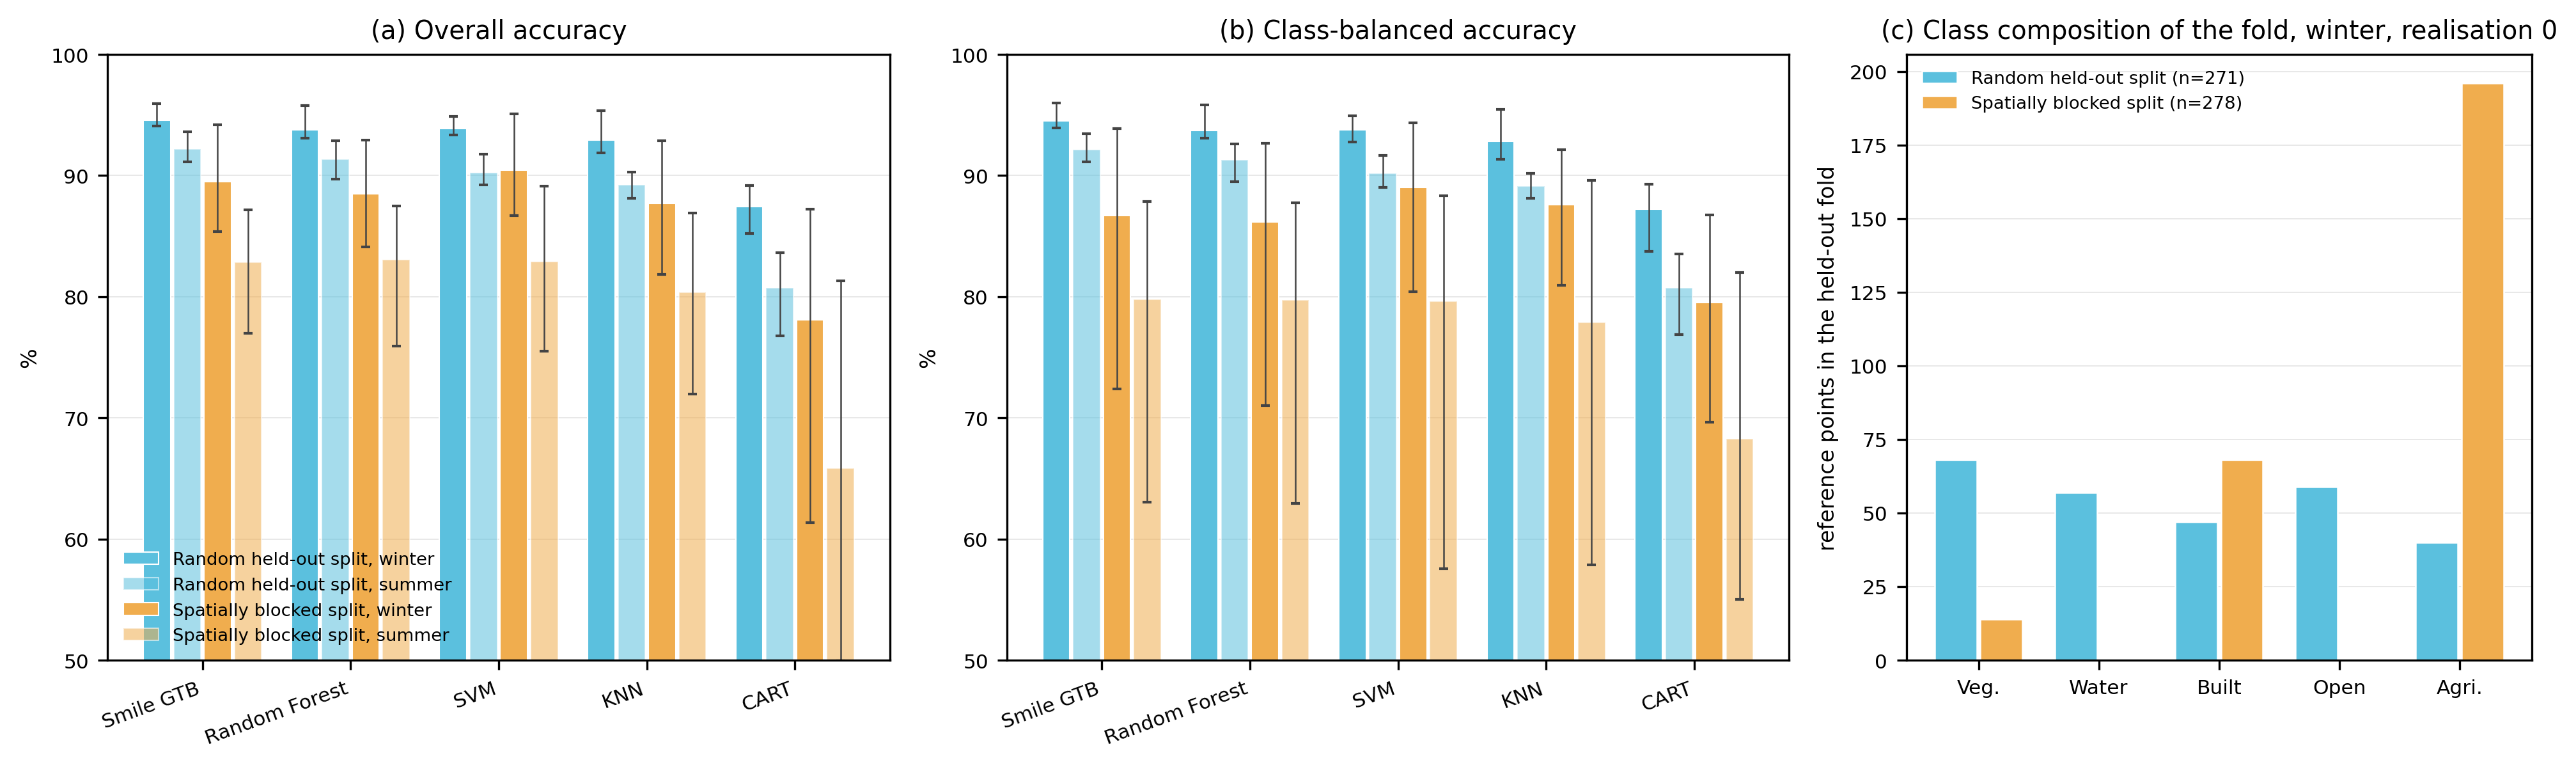
\includegraphics[width=0.95\textwidth]{fig_protocols.png}
\caption{The validation protocol over eight realisations. (a) Overall accuracy of all five classifiers under a random and a contiguous spatially blocked partition of the same labelled points, in both seasons; each bar is the mean over the eight rotations of the held-out bands and the whisker their full range. (b) The same runs by class-balanced accuracy. (c) Why one realisation is not enough: realisation~0 holds out a band that is almost entirely agriculture, against a random fold of the same size that inherits the training set's balance, so part of any single-realisation difference in (a) is a difference in what is being classified. Every count is read from \texttt{jabalpur\_split\_protocols\_v3.json}, which stores each confusion matrix beside the metrics derived from it.}
\label{fig:protocols}
\end{figure*}

Table~\ref{tab_protocols} and Fig.~\ref{fig:protocols} report the same five models under a random and a spatially blocked partition of the same labelled points, on the production \texttt{sel19} stack and the frozen hyperparameters of Table~\ref{tab_hyper}. Three things about the design decide what the numbers mean. The blocked partition is ten contiguous longitudinal bands across the labelled extent, $0.1204^\circ$ or about 12.3\,km wide, with three held out, so it controls autocorrelation over a whole band rather than leaking at every cell boundary as the hashed 0.1-degree assignment of earlier versions did. The experiment is repeated over eight rotations of the held-out window, so one arbitrary choice of ground is not mistaken for the effect. And in each realisation both protocols are given the same number of training rows and the same held-out size, so training budget is not confounded with partition geometry.

Under that design the protocol effect in winter is $+5.09$ points for the leading model, standard deviation 3.46 across realisations, and between $+3.41$ and $+9.35$ across the five classifiers, a mean of $+5.67$. In summer it is $+9.33 \pm 4.21$ for the leading model and $+9.75$ on average across classifiers. Two features of that are as important as the means. The effect is much larger than the $+3.41$ winter figure the hashed-block design produced, which confirms in measurement what that design predicted in principle: a partition that leaks at every boundary understates the protocol effect. And the spread across realisations is wide---the winter effect ranges from $-1.54$ to $+11.53$ points for the same classifier depending on which bands are held out, and CART reaches $+26.54$ in one realisation---so a protocol effect quoted from a single blocked split is not a stable quantity. That is the reason this table reports eight.

Two qualifications keep the comparison honest. First, both labelled-set protocols score agreement with the project's own labels while the external rows score an independent reference, so the distance between the two blocks of the table is a change of yardstick as well as of protocol, and the external assessment additionally changes geography, reference construction and sample design. Second, the two partitions still do not hold out the same class mixture: a contiguous band of the labelled region has whatever composition that ground has, and realisation~0 holds out 195 agriculture points and no water or open land at all, against a random fold of the same size that inherits the training set's balance (Fig.~\ref{fig:protocols}c). Class-balanced accuracy, which is invariant to that mixture, does not remove the effect and in this design slightly increases it: $+7.78$ points for the leading model in winter and $+12.37$ in summer, against $+5.09$ and $+9.33$ on overall accuracy. The protocol effect survives standardisation.

\section{Discussion}

\subsection{What the feature families contribute}
The ablation of Section~\ref{sec:families} puts a number on something usually asserted: optical bands and their core indices alone reach 75.9\% overall accuracy on the development districts but only 42.0\% recall for open land, and adding five further bareness and built-up indices moves that recall down rather than up. That is the diagnostic result, and it is consistent with a straightforward reading: indices built from the same six reflectance bands add no measurement that those bands did not already carry. What the ablation then shows is that the two families measuring something other than per-pixel brightness---grey-level texture and radar---are where the open-land recall comes from, 16.6 points and 16.0 points respectively in winter. The mechanism usually offered for the radar half is double-bounce scattering from a wall-and-ground corner, which has no reflectance analogue. That is a plausible account and the one the feature was chosen for, but the experiment measures predictive contribution on this reference and does not isolate a scattering mechanism; the season-dependence is the reason to be careful about the stronger reading, since the same family is worth 16.0 points of open-land recall in winter and 1.3 in summer, which a purely geometric explanation would not predict. One further qualification applies to every open-land number in this paper and is not a matter of degree. The independent arbiter of Table~\ref{tab_arbiter} agrees with the consensus open-land label on 28.1\% of winter points and 17.4\% of summer ones, calling most of the rest cropland. The ablation therefore measures how much texture and radar improve agreement with a label that a comparable product mostly rejects, and whether a model that called those pixels cropland instead would be closer to the ground is a question this design cannot reach. 

\subsection{Texture and radar act on different errors}
Texture and radar move different parts of the same confusion, and the ablation separates them. Adding optical GLCM texture raises built-area precision from 57.5\% to 62.5\% while lifting open-land recall by 16.6 points, which is consistent with it declining to call a smooth surface built. Adding radar then lifts open-land recall by a further 16.0 points at a built-area precision of 73.1\%. Neither substitutes for the other in these measurements, and the leave-one-family-out sweep of Fig.~\ref{fig:ablation} agrees: removing either costs accuracy in both seasons, and removing SAR amplitude costs the most of any family. All of these are predictive contributions measured against the consensus reference on the development districts, and none is a physical measurement of a surface property. 

\subsection{Re-evaluating accuracy assessment paradigms}
\label{sec:protocols}
Table~\ref{tab_protocols} carries a result worth stating carefully rather than broadly. The same models, on the same composite and the same feature stack, give answers that differ by about five points in winter and about ten in summer according only to how the held-out set was drawn. That is enough to make a randomly split figure and a spatially split figure incomparable. It is not enough to support the stronger claim that the protocol matters more than the classifier: on these same folds the five classifiers span 7.14 points on the random partition and 12.37 on the blocked one in winter, against a 5.67-point protocol effect, and 11.44 and 17.21 in summer against 9.75.

The mechanism is measurable in this label set: the median nearest-neighbour distance within the open-land class is 29\,m, and 984 of its 1,000 points lie within 100\,m of another point of the same class. On a 10\,m grid that median is under three cells, and 100\,m is ten, so a random split routinely places a training point and a test point within a few pixels of each other, and what the reported figure measures is partly the model's ability to interpolate between neighbours it has already seen. This is not a defect peculiar to this dataset \cite{r18}, \cite{r19}. Any label set collected by digitising polygons has the same structure, and a randomly split accuracy from such a set is not comparable with a spatially blocked one, whatever the two numbers look like side by side.

What the repeated realisations add is a warning about how such an effect is usually reported. A single blocked split of this label set gives a winter protocol effect anywhere between $-1.5$ and $+11.5$ points for one classifier, depending on which ground it happens to hold out. A study that runs one blocked split and quotes its gap is quoting a draw from that distribution. The standard deviations in Table~\ref{tab_protocols}, 3.4 to 10.6 points, are the honest width of the claim.

The further step, from either local protocol to the external consensus over 29 held-out districts, changes geography, reference construction and sampling design at the same time, so its size is not attributable to the validation protocol and is not claimed to be.

\subsection{Limitations and future directions}
\label{sec:limits}
These results are bounded by the following limits, and each is a property of the design rather than a caveat added afterwards.

\begin{enumerate}
    \item The reference is an agreement domain formed from existing maps rather than an independently interpreted field or very-high-resolution sample, and the agreement required of a pixel depends on which class it is a candidate for (Eq.~\eqref{eq:refrules}). Shared source data, product-epoch differences, excluded classes and unequal per-class screening can introduce correlated and selective reference error, and the selection is not neutral between classes: agriculture enters the reference on the weakest condition and occupies the most area, while vegetation enters on the strictest and nearly vanishes in summer. Because Dynamic World is itself derived from Sentinel-2, the reference and the classifiers also share an observation source, so agreement between them is not independent evidence. The class-specific arbiter comparison of Table~\ref{tab_arbiter} puts the sharpest version of this limit on record: open land, the class the feature stack exists to separate, carries a reference label an independent product of comparable standing assigns to only 28.1\% of the same points in winter and 17.4\% in summer. That is disagreement between two products and identifies neither as correct, but it means no open-land figure here can be read as an accuracy. No experiment reported here separates a classifier error from a reference-screening artefact, and none of the figures is corrected for reference error. The consensus-rejected half of the state is sampled only by a three-district, 120-point pilot, and no independently interpreted audit has been carried out at all. Every accuracy in this paper is therefore conditional map agreement.
    \item The reference epochs do not match the 2025 composites and are not uniform among themselves: 2018 for the built-surface specialist, 2021 for WorldCover and WorldCereal, 2024 for the arbiter. Rapidly changing urban peripheries are where that spread will show.
    \item Training labels are spatially clustered inside four historical districts, and the median nearest-neighbour distance within the open-land class is 29\,m. Their original per-point interpretation metadata were not retained: no interpreter, source image or date attribute survives on the assets, so per-point provenance cannot be reconstructed and no second-annotator agreement can be computed after the fact. Open-land labels in particular come from one region, and targeted labels elsewhere would probably buy more than uniform additional labelling.
    \item The hyperparameter grid is deliberately small and covers the capacity controls that matter most for these five models. It is not an exhaustive search, and a wider one on the same development districts could still move the ranking among the top three, which this evidence already cannot separate.
    \item The reported figures carry a fitting band that the sampling intervals do not describe. Given a fixed training table every classifier here reproduces exactly, and a fresh native re-run reproduces the stored winter figure exactly for Smile GTB and SVM; but permuting the training rows, or merely transporting the same values through a different representation, moves pooled agreement by up to 0.38 points for the leading model and 0.76 for SVM, changing over a hundred individual predictions. Nothing in this workflow pins the composition, order and numeric representation of the training table across sessions, so the headline figure carries a band of that order, comparable to the winter margins separating it from the next two classifiers. The $D=531$ discrepancy in the archived rebuild is not explained by this and remains unexplained.
    \item Neither agreement estimate describes Madhya Pradesh. The unweighted one describes a landscape that is one fifth water by design, and the area-weighted one describes the consensus domain, which is 56.5\% of the test districts' area and 95.86\% agriculture by area in winter. That composition is an artefact of Eq.~\eqref{eq:refrules}---the least strictly screened class is also the largest---and it is why a constant agriculture predictor outscores the trained pipeline on the weighted estimator, and why weighted user's accuracy for built area and open land is under 5\% (Section~\ref{sec:area}, Table~\ref{tab_weighted_class}). No conclusion about mapping those two classes can rest on the weighted figures, and a genuine map-wide estimate would need a fresh sample stratified on the map's own classes.
    \item The protocol comparison of Table~\ref{tab_protocols} now runs on the production stack, over contiguous bands, with matched training budgets and eight realisations, but one band width was tested and not several. The bands are the labelled extent divided by ten, $0.1204^\circ$ of longitude or about 12.3\,km, so the design controls autocorrelation at that scale and says nothing about what a 25\,km or 50\,km block would show. The realisation spread is also wide enough (standard deviations of 3.4 to 10.6 points) that eight realisations pin the mean effect only loosely. A sweep over block widths, with more realisations at each, is the remaining work on this question.
    \item The texture footprint is now measured rather than assumed (Section~\ref{sec:texture_grid}), and what the measurement shows is a property of the workflow that no accuracy figure removes: the composite carries a default projection, so the GLCM neighbourhood is fixed by the request rather than by the feature code. Training and evaluation both request 10\,m and both therefore see a 70\,m footprint, which is what the reported results rest on. The delivered dashboard raster does not: its render scale is the drawn polygon's width divided by at most 2,048 pixels, so an area wider than about 20\,km is classified from texture measured over a coarser neighbourhood than the model was fitted on. That is a mismatch between the assessed product and the served one, and it is not corrected here. Pinning the grey-level images to an explicit grid with \texttt{reproject} would remove it at a compute cost that has not been measured.
    \item The summer evaluation sample is not class-balanced. The consensus yields 372 vegetation points against 580 of each other class, so pooled summer agreement of 73.85\% and class-balanced summer accuracy of 71.71\% are different quantities and both are reported; the winter sample is balanced and its two figures coincide. The two seasons are also not scored on the same reference domain, the summer vegetation stratum having fallen to 0.12\% of the covered area. Section~\ref{sec:fixed} recovers a fixed-location, fixed-label comparison from the 1{,}350 points the two samples share, and the fall there is 8.67 points against 13.56 pooled; but that subset holds four vegetation points, so the control cannot speak to the class that drives the headline gap, and it still refits the model per season rather than holding it fixed.
    \item Results cover two 2025 seasons within Madhya Pradesh and should not be generalised to other states or years without further testing. The differences between seasons also include changes in reference coverage and sample composition, not phenology alone.
    \item Reported accuracy applies to the raw per-pixel classification. The majority-filtered raster the dashboard delivers is now measured separately (Section~\ref{sec:delivered}) and agrees slightly better with the reference sample while losing 14.7\% of the mapped water area in Jabalpur, so the two products are not interchangeable for area statistics. Two further properties of the served path remain unmeasured: the temporally widened window it may fall back to when a polygon returns no imagery, and its coarser texture footprint for polygons wider than about 20\,km.
\end{enumerate}

Two directions follow from these limits rather than from the results. The first, and the one that would change most, is a small independent reference audit outside the mechanism that built the consensus: reference locations chosen by a declared probability design from both consensus-accepted and consensus-rejected areas, before any model prediction is inspected, interpreted on dated 2025 high-resolution imagery by two readers with predictions hidden, with inclusion probabilities, disagreements and adjudicated labels retained. A planning budget of 500 to 800 locations across 8 to 12 geographically diverse test districts is illustrative rather than power-derived, and would support inference only over the sampled domain; at 100 points the worst-case independent-binomial 95\% half-width is already about 9.8 percentage points, and clustering would widen it. That is the only route from a bounded reference-uncertainty figure to a corrected accuracy. The second is active learning over the open-land class specifically: it is the class the feature stack exists to repair, the one whose recall is weakest away from the labelled area, and the one for which the training labels come from a single region, so targeted labels in Malwa, Chambal and Bundelkhand should buy more than uniform additional labelling anywhere else.

\FloatBarrier
\section{Conclusion}
This paper assessed a five-class land use/land cover workflow in Google Earth Engine, driven by machine learning on Sentinel-2 and Sentinel-1 and evaluated under a spatial partition that keeps every modelling choice off the data used to report it. Three results survive that partition. Optical reflectance and the indices built from it do not separate dry open land from built area on this reference, reaching 42.0\% open-land recall in winter, and adding five further bareness and built-up indices does not repair it; grey-level texture and Sentinel-1 backscatter take that recall to 73.3\% in winter, though the incremental radar contribution is much smaller in summer. Feature composition matters more than feature count: two 19-band stacks of identical size differ by 1.76 points in winter and 4.91 in summer on ground neither was chosen on. Smile GTB reached 87.41\% sample agreement (95\% CI 85.07--89.69\%) and Kappa 0.843 in winter across 29 held-out test districts, on a winter sample that is exactly class-balanced so that the pooled and class-balanced readings coincide, against 73.85\% pooled and 71.71\% class-balanced in summer, a margin that multiplicity-adjusted paired district tests do not separate from SVM or Random Forest, and which is therefore not a claim that Smile GTB is the best classifier nor that the three are equivalent. Two independent facts point the same way: the adjusted $p$ values against both comparators are 0.125, and permuting the order of the training rows, changing no value, moves the model's own accuracy by 0.38 points and 119 individual predictions, which is the size of the margin being argued over. Area-weighted over the domain the reference actually covers, which is 56.5\% of those districts' area and 95.86\% of it agriculture, the same result is 75.50\% $\pm$ 3.32, below the 95.86\% a constant agriculture predictor scores on that estimator; the weighted figure describes agreement over a reference-defined domain and not the usefulness of the map.

Two of those numbers carry further than any of the accuracies. The difference between the sample-weighted and area-weighted readings of one set of predictions is larger than the difference between any two classifiers here, so how a reference sample is weighted decides more than which model is trained. And on the same labelled points, the same composite, the same feature stack and the same frozen configuration, moving from a random partition to a contiguous spatially blocked one costs a mean of 5.67 points in winter and 9.75 in summer, over eight rotations of the held-out bands with the training budget matched in each. That effect is real, and it is larger than the 3.41 points a hashed 0.1-degree block assignment reported, which is what a partition that leaks at every cell boundary does to a protocol contrast. It is not, however, larger than the effect of choosing a classifier: in winter the five classifiers span 7.14 points on the random partition and 12.37 on the blocked one, and in summer 11.44 and 17.21, against protocol effects of 5.67 and 9.75. The other thing eight realisations show is how loosely a single blocked split pins any of this down: for one classifier the winter effect ranges from $-1.5$ to $+11.5$ points depending only on which bands are held out. The honest statement is the narrow one, that on this label set a contiguous spatial partition moved the reported accuracy by several points in the same direction for every classifier, that the size of that move is not stable across realisations, and that it remains smaller than the spread between classifiers. What none of this establishes is verified accuracy: the reference is a consensus of public maps that shares its observation sources with the classifiers and excludes the pixels those maps dispute, so every figure here is conditional agreement over a stated domain, and an independent reference audit remains the work that would change the answer rather than the wording.

\section*{Data and Code Availability}
The source satellite and public-map products are available from the providers identified in the reference inventory. The optical composites come from \texttt{COPERNICUS/S2\_SR\_HARMONIZED} and the radar from \texttt{COPERNICUS/S1\_GRD}. District boundaries are FAO GAUL 2015 level~2. The reference consensus is built from ESA WorldCover v200, Dynamic World, OPERA DSWx-HLS, the JRC GHSL P2023A built-surface layer and ESA WorldCereal 2021, at the epochs and native grids given in Section~\ref{sec:accuracy}, and is audited against the ESRI 10\,m Annual Land Cover product for 2024. The legend crosswalk that turns those products into the five classes, including the classes deliberately left unassigned, is Table~\ref{tab_crosswalk}; the consensus cannot be rebuilt without it. The public availability of the source imagery alone is not sufficient for reproduction: that also requires the manually interpreted training points, the district split, the reference-generation rules, the preprocessing configuration and the evaluation scripts.

Every number, table and figure in this paper is generated from a frozen archive of flat files rather than transcribed. The archive sits beside the code that reads it, under \texttt{doc/assets/result\_archive/} at the commit recorded in \texttt{experiment\_manifest.csv}, \texttt{b394786}. \emph{[Author action before submission: a citable location for that commit---a repository URL or a deposited archive with a DOI---belongs here. File names without a location are not a reproduction package, and this section is not complete without one.]} The files are these:

\begin{itemize}
    \item \texttt{experiment\_manifest.csv} --- one row per run, with the training season, feature stack, hyperparameters, evaluation population, selection objective and whether the run influenced any choice.
    \item \texttt{district\_split.csv} --- every GAUL ADM2 unit with its role, block identifier, centroid, per-season sample count, district area and consensus-covered area.
    \item \texttt{district\_confusion\_matrices.csv} --- the full $5\times5$ matrix for every district, season and model, with its source file and schema version.
    \item \texttt{metrics.csv} --- pooled overall accuracy, Kappa, macro F1 and per-class precision, recall and F1 for every run, each recomputed from the matrix above.
    \item \texttt{stratum\_areas.csv} --- eligible area and sample count for every (season, district, consensus class) stratum, with the exclusion reason where a stratum has area and no sample.
    \item \texttt{reference\_domain\_coverage.csv} --- district area, covered area and both agreement estimates with the uncertainty method, per season and population.
    \item \texttt{paired\_contrasts.csv} --- all eight paired comparisons with interval, raw and Holm-adjusted $p$, tie and zero counts, and the test variant used.
    \item \texttt{feature\_experiments.csv} --- every cumulative, leave-one-band-out, leave-one-family-out and candidate-stack run, each with its source file and whether it predates the hyperparameter search, so that two figures for ``the same stack'' can be told apart.
    \item \texttt{spatial\_transfer.csv} --- per-district distance from Jabalpur and accuracy, with the distance regression fitted separately on all 44 evaluation districts and on the 29 test districts alone.
    \item \texttt{predictions.csv} --- one row per sampled reference pixel, with its coordinates, stratum, reference label and one predicted label per model, so that a stratum weight can be recomputed, the sample re-stratified, or a single disputed pixel located. This file is the \emph{re-run} audit record and not the frozen evaluation: the frozen run preserved confusion matrices and no per-point predictions, and the two are deliberately kept as separate records rather than merged.
    \item \texttt{reproduction\_check.csv} --- the stored evaluation against an independent re-run of the same sample, district by district and model by model.
    \item \texttt{protocol\_comparison.csv} --- every model under both split protocols in both seasons, with training size, fold size and fold class composition.
    \item \texttt{reference\_inventory.csv} --- each reference product with its asset identifier, version, epoch, native grid, specialist condition and remap.
    \item \texttt{pairwise\_contrasts\_all.csv} --- all ten pairwise classifier contrasts per season, with the family used for the multiplicity adjustment.
\end{itemize}

Five records were added for this revision and sit beside the archive rather than in it, because each answers one audit question rather than feeding a table:

\begin{itemize}
    \item \texttt{texture\_grid\_audit.json} --- the projection, transform and nominal scale of every stage of the feature stack, the texture values at five request scales, and the render scale of the delivered raster by polygon width.
    \item \texttt{refit\_variability.json} --- every repeated fit, under a frozen table, a permuted row order and a re-sampled table, with the changed-prediction counts.
    \item \texttt{fixed\_location\_seasonal.json} --- the 1{,}350 locations sampled in both seasons under an unchanged reference label, per class and per model.
    \item \texttt{reference\_shortfall\_audit.json} --- every stratum that missed the sampling quota, with its eligible area and what was drawn.
    \item \texttt{delivered\_map\_eval\_\{season\}.json} and \texttt{rejected\_domain\_audit.json} --- the agreement of the majority-filtered raster the dashboard serves over all 29 test districts, and the three-district pilot comparing the consensus-accepted and consensus-rejected halves of the state against an independent product.
\end{itemize}

The completed \texttt{predictions.csv} contains 9{,}281 rows over all 96 district-seasons and all eight frozen model/stack columns. The audit reconstruction differs from the stored confusion matrices by a redistribution statistic of 535. That quantity has to be named precisely, because it is not a count of point-level prediction changes. What the rebuild computes is
\begin{equation}
D \;=\; \tfrac{1}{2}\sum_{a,b}\bigl|\,C^{\mathrm{rerun}}_{ab}-C^{\mathrm{stored}}_{ab}\,\bigr|,
\label{eq:matrixdist}
\end{equation}
the half $L_1$ distance between two confusion matrices of equal total. $D$ counts how much probability mass moved between cells, not how many individual pixels changed label, and the two differ: if two sampled pixels of the same reference class exchange predicted labels, both predictions have changed and $D$ is zero. Under matched samples and matched reference labels $D$ is a lower bound on the number of changed predictions, and it is reported here as such. The exact pointwise figure cannot be recovered from this archive, because the frozen run preserved confusion matrices and not per-point predictions; \texttt{predictions.csv} carries a \texttt{sample\_id} for every row of the re-run, so the join that would give the exact count is available prospectively but has no stored counterpart to join against. Reconstructing the frozen run at row level, and reporting the true pointwise disagreement, is outstanding work.

The rebuild asserts, for every matrix it prints a metric from, that $n$ is the matrix sum, that overall accuracy is the trace over that sum, and that each per-class precision, recall and F1 is the corresponding ratio of counts, so a figure and a table cannot report different values for one run. Superseded records are retained rather than overwritten: the split-protocol experiment appears as both its original archive and the re-run that stores confusion matrices, and the two are distinct files.

Four of the records added for this revision---the fixed-location seasonal comparison, the repeat-fit experiment, the delivered-raster evaluation and the rejected-domain audit---are computed on predictions generated for them rather than restored from the frozen run, because the frozen run preserved matrices and not per-point predictions. Each is labelled as such where it is reported, and none of them changes a headline accuracy: they are audits of what the headline figures mean.

Two of those files are records of different kinds, and the distinction is worth stating. What this paper reports is the frozen evaluation, and it stays that way: re-running a held-out evaluation after its results have been read, and then reporting the re-run, is how a held-out set stops being held out whatever the intention. The row-level table is an audit record drawn afterwards, by rebuilding the same seeded sample and classifying it again.

It does not reproduce the stored run to the last pixel, and \texttt{reproduction\_check.csv} publishes the difference rather than absorbing it. The difference is concentrated: $D=1$ for each of Random Forest, SVM, KNN and CART, in the same district, against $D=531$ for Smile GTB. Section~\ref{sec:models} reports the controlled experiment that this comparison could not substitute for. Its result is that the fit is deterministic given a fixed training table, that a fresh native re-run reproduces the stored Smile GTB figure to every digit, and that the fit moves when the table's row order or representation does not hold. The rebuild is an uncontrolled comparison, so it locates a discrepancy rather than explaining one, and no claim is made here about the reproducibility of Earth Engine studies in general. And the archive's own provenance is weaker than it should be, since \texttt{experiment\_manifest.csv} records its \texttt{code\_commit} field by reference to the repository history rather than as an immutable commit hash; the commit is \texttt{b394786}, and pinning it in the manifest itself is a correction this version makes.

Three further details fix parts of the protocol that a description alone would leave ambiguous. The seasonal windows are the half-open intervals of Section~\ref{sec:seasons}. The development/test partition is deterministic and seedless: each district centroid falls in a one-degree block, and a block joins the development half when the sum of its integer row and column indices is divisible by three, which spreads development blocks across the state's full longitude range instead of carving off a corner. All bootstrap intervals are percentile intervals over 5{,}000 replicates that resample whole districts with replacement, drawn with seed 20260901; the area-weighted intervals are design-based and are not bootstrapped.

Model settings, candidate feature stacks and planned comparisons were fixed before the final evaluation records were examined. The test set was used to estimate performance and to report those pre-specified contrasts; it was not used to choose a new configuration. Any analysis influenced by earlier access to the same records is identified as exploratory, which in this paper means the distance regression of Section~\ref{sec:spatial}. Earlier statewide evaluations were run before the present split existed, and they informed the decision to partition the districts at all; they contributed no feature, model or hyperparameter choice, and none of their numbers is reported here.

The 5,000 labelled training points are the only non-public input. They are five Earth Engine feature collections under a private asset root---\texttt{jabalpur\_\{forest,water,building,barren\}\_points} and \texttt{jabalpur\_agriculture\_points\_labelled}---each carrying an integer class label, and they are not currently released. \emph{[Author action before submission: state the access mechanism the authors are willing to commit to---deposit, sharing on request, or none---since the reviewer's objection is to the absence of a stated mechanism, not to the labels being private.]} Their class counts, spatial extent, distinct-location counts and nearest-neighbour statistics are reported in Section~\ref{sec:labels} so that a comparable set can be constructed independently, but that is a substitute for the labels and not the labels themselves, and this paper does not claim to be reproducible end to end without them.

\section*{Corrections to the Previous Version}
Correction notices that were previously carried inline are collected here so that the body of the paper states what it now finds rather than what it used to. Nothing in this list is needed to read the results.

\begin{enumerate}
    \item \textbf{Reference construction.} The crosswalk caption said a pixel unassigned in either general product cannot enter the reference. Agriculture never consults Dynamic World, so only WorldCover exclusions apply to it. The text also attributed seasonal change in the agriculture reference to Dynamic World; the agriculture mask is static in its entirety and its eligible area is identical in both windows, district by district.
    \item \textbf{Texture grid.} The GLCM footprint was described and not verified. Section~\ref{sec:texture_grid} now records the projection at every stage and measures the footprint, and reports the mismatch between the assessed raster and the raster the dashboard delivers for a large polygon.
    \item \textbf{Area weights.} The stratum areas that weight the design-based estimator were measured at 30\,m for a sample drawn at 10\,m. They are now measured on the sampling grid and every weighted figure, coverage percentage and interval is recomputed from them. The weighted overall estimates barely move, 75.50\% and 58.67\% against 75.50\% and 58.69\%, but the minority classes gain the domain share the coarse grid hid, the two summer accounting defects disappear, and one conclusion reverses: the apparent sampling anomaly in Bhind was an artefact of the 30\,m measurement.
    \item \textbf{Reproducibility.} The difference between the frozen run and its rebuild was described as a count of changed point predictions. It is a confusion-matrix redistribution statistic, and it is now named as one. The assertion that Smile GTB is not run-to-run reproducible is replaced by the controlled repeat-fit experiment of Section~\ref{sec:models}, which shows the fit deterministic given a fixed training table and shows a fresh native re-run reproducing the stored Smile GTB figure exactly.
    \item \textbf{Protocol comparison.} It ran on the \texttt{alt19} stack, under a 0.1-degree block assignment scrambled by an integer hash, on one realisation, and was captioned as \texttt{sel19}. It now runs on \texttt{sel19}, over contiguous bands, with matched training budgets, on eight realisations.
    \item \textbf{Summer vegetation shortfall.} Attributed first to agriculture and open-land disagreement, then to scarcity in the reference. Both were incomplete: Table~\ref{tab_shortfall} audits it per district.
    \item \textbf{Baselines and the weighted estimator.} The constant-class baseline on the pooled summer sample is 21.55\%, not 20\%. The weighted estimator is not maximised by a constant agriculture map---perfect agreement would score 100\%---it merely ranks that map above the trained one.
    \item \textbf{Scaling bounds.} Described as 1st-to-99th percentile stretches. The implemented lower bound is exactly zero and the upper bound is a rounded 99th percentile, held fixed across every fold, which is also declared as a small leak in the labelled-fold protocols.
    \item \textbf{Distance conversion.} On a 10\,m grid 100\,m is ten pixels, not three.
    \item \textbf{Classifier contrasts.} The statement that CART is separated from every other classifier was made from a family that contained no CART-versus-non-leader contrast. All ten pairs are now tested (Table~\ref{tab_pairwise_all}), which supports that statement and weakens the summer separation of the leading model from Random Forest.
    \item \textbf{Reference error by class.} Only the aggregate arbiter agreement was reported. Table~\ref{tab_arbiter} gives it by class, where open land turns out to be contested at a rate the aggregate hides entirely.
    \item \textbf{Figure~\ref{fig:methodology}} said ``compute 19 features'' and ``48 districts'' against a caption describing 27 candidates and 29 test districts, and drew no development or test lane. It has been redrawn.
    \item \textbf{Smaller corrections.} Table~\ref{tab_lit} listed a single-classifier study as a multi-classifier comparison; the per-class F1 ordering was misreported; a 0.26-point offset was claimed between two tables that their own rows contradict; wetland, flooded-vegetation and mangrove codes were shown as mapped into water and vegetation, which the implementation never did; physical claims about double-bounce scattering and about cloud contamination being shared between seasons are now qualified to what was measured; and the availability section now names the commit and marks the citable location and the label-access mechanism as author actions rather than leaving the omission silent.
\end{enumerate}

\clearpage
\begin{thebibliography}{00}
\bibitem{r1} J. W. Rouse et al., ``Monitoring vegetation systems in the Great Plains with ERTS,'' \textit{NASA Special Publication}, vol. 351, p. 309, 1974.
\bibitem{r2} C. J. Tucker, ``Red and photographic infrared linear combinations for monitoring vegetation,'' \textit{Remote Sens. Environ.}, vol. 8, no. 2, pp. 127--150, May 1979.
\bibitem{r3} Z. Zhao et al., ``Comparison of three machine learning algorithms using Google Earth Engine for land use land cover classification,'' \textit{Rangel. Ecol. Manag.}, vol. 92, pp. 129--137, Jan. 2024.
\bibitem{r4} M. Drusch et al., ``Sentinel-2: ESA's optical high-resolution mission for GMES operational services,'' \textit{Remote Sens. Environ.}, vol. 120, pp. 25--36, May 2012.
\bibitem{r5} D. Phiri et al., ``Sentinel-2 data for land cover/use mapping: a review,'' \textit{Remote Sens.}, vol. 12, no. 14, p. 2291, Jul. 2020.
\bibitem{r6} R. Torres et al., ``GMES Sentinel-1 mission,'' \textit{Remote Sens. Environ.}, vol. 120, pp. 9--24, May 2012.
\bibitem{r7} M. Pal and P. M. Mather, ``Support vector machines for classification in remote sensing,'' \textit{Int. J. Remote Sens.}, vol. 26, no. 5, pp. 1007--1011, Mar. 2005.
\bibitem{r8} A. E. Maxwell, T. A. Warner, and F. Fang, ``Implementation of machine-learning classification in remote sensing: an applied review,'' \textit{Int. J. Remote Sens.}, vol. 39, no. 9, pp. 2784--2817, May 2018.
\bibitem{r9} P. O. Gislason, J. A. Benediktsson, and J. R. Sveinsson, ``Random forests for land cover classification,'' \textit{Pattern Recognit. Lett.}, vol. 27, no. 4, pp. 294--300, Mar. 2006.
\bibitem{r10} N. Gorelick et al., ``Google Earth Engine: planetary-scale geospatial analysis for everyone,'' \textit{Remote Sens. Environ.}, vol. 202, pp. 18--27, Dec. 2017.
\bibitem{r11} L. Breiman, ``Random forests,'' \textit{Mach. Learn.}, vol. 45, no. 1, pp. 5--32, Oct. 2001.
\bibitem{r12} C. Cortes and V. Vapnik, ``Support-vector networks,'' \textit{Mach. Learn.}, vol. 20, no. 3, pp. 273--297, Sep. 1995.
\bibitem{r13} T. Chen and C. Guestrin, ``XGBoost: a scalable tree boosting system,'' in \textit{Proc. 22nd ACM SIGKDD}, Aug. 2016, pp. 785--794.
\bibitem{r14} D. Zanaga et al., ``ESA WorldCover 10 m 2021 v200,'' Zenodo, 2022.
\bibitem{r15} C. F. Brown et al., ``Dynamic World, near real-time global 10 m land use land cover mapping,'' \textit{Sci. Data}, vol. 9, p. 251, Jun. 2022.
\bibitem{r16} J. Van Tricht et al., ``WorldCereal: a dynamic open-source system for global-scale, seasonal, and reproducible crop and irrigation mapping,'' \textit{Earth Syst. Sci. Data}, vol. 15, no. 12, pp. 5491--5515, Dec. 2023.
\bibitem{r17} P. Olofsson et al., ``Good practices for estimating area and assessing accuracy of land change,'' \textit{Remote Sens. Environ.}, vol. 148, pp. 42--57, May 2014.
\bibitem{r18} D. R. Roberts et al., ``Cross-validation strategies for data with temporal, spatial, hierarchical, or phylogenetic structure,'' \textit{Ecography}, vol. 40, no. 8, pp. 913--929, Aug. 2017.
\bibitem{r19} P. Ploton et al., ``Spatial validation reveals poor predictive performance of large-scale ecological mapping models,'' \textit{Nat. Commun.}, vol. 11, p. 4540, Sep. 2020.
\bibitem{r20} R. M. Haralick, K. Shanmugam, and I. Dinstein, ``Textural features for image classification,'' \textit{IEEE Trans. Syst. Man Cybern.}, vol. SMC-3, no. 6, pp. 610--621, Nov. 1973.
\bibitem{r21} Y. Zha, J. Gao, and S. Ni, ``Use of normalised difference built-up index in automatically mapping urban areas from TM imagery,'' \textit{Int. J. Remote Sens.}, vol. 24, no. 3, pp. 583--594, Feb. 2003.
\bibitem{r22} S. K. McFeeters, ``The use of the normalised difference water index (NDWI) in the delineation of open water features,'' \textit{Int. J. Remote Sens.}, vol. 17, no. 7, pp. 1425--1432, May 1996.
\bibitem{r23} H. Xu, ``A new index for delineating built-up land features in satellite imagery,'' \textit{Int. J. Remote Sens.}, vol. 29, no. 14, pp. 4269--4276, Jul. 2008.
\bibitem{r24} A. R. Huete, ``A soil-adjusted vegetation index (SAVI),'' \textit{Remote Sens. Environ.}, vol. 25, no. 3, pp. 295--309, Aug. 1988.
\bibitem{r25} A. Rikimaru, P. S. Roy, and S. Miyatake, ``Tropical forest cover density mapping,'' \textit{Tropical Ecology}, vol. 43, no. 1, pp. 39--47, 2002.
\bibitem{r26} A. Rasul et al., ``Applying built-up and bare-soil indices from Landsat 8 to cities in dry climates,'' \textit{Land}, vol. 7, no. 3, p. 81, Jul. 2018.
\bibitem{r27} J. H. Friedman, ``Greedy function approximation: a gradient boosting machine,'' \textit{Ann. Statist.}, vol. 29, no. 5, pp. 1189--1232, Oct. 2001.
\bibitem{r28} J. Cohen, ``A coefficient of agreement for nominal scales,'' \textit{Educ. Psychol. Meas.}, vol. 20, no. 1, pp. 37--46, Apr. 1960.
\bibitem{r29} M. Kawamura, S. Jayamana, and Y. Tsujiko, ``Relation between social and environmental conditions in Colombo, Sri Lanka, and the urban index estimated by satellite remote sensing data,'' \textit{Int. Arch. Photogramm. Remote Sens.}, vol. 31, pt. B7, pp. 321--326, 1996.
\bibitem{r30} S. Bouzekri, A. A. Lasbet, and A. Lachehab, ``A new spectral index for extraction of built-up area using Landsat-8 data,'' \textit{J. Indian Soc. Remote Sens.}, vol. 43, no. 4, pp. 867--873, Dec. 2015.
\bibitem{r31} W. R. Tobler, ``A computer movie simulating urban growth in the Detroit region,'' \textit{Econ. Geogr.}, vol. 46, sup1, pp. 234--240, Jun. 1970.
\bibitem{r32} G. F. Hughes, ``On the mean accuracy of statistical pattern recognizers,'' \textit{IEEE Trans. Inf. Theory}, vol. 14, no. 1, pp. 55--63, Jan. 1968.
\bibitem{r33} G. De Luca, J. M. N. Silva, S. Di Fazio, and G. Modica, ``Integrated use of Sentinel-1 and Sentinel-2 data and open-source machine learning algorithms for land cover mapping in a Mediterranean region,'' \textit{Eur. J. Remote Sens.}, vol. 55, no. 1, pp. 52--70, Dec. 2022.
\bibitem{r34} S. Holm, ``A simple sequentially rejective multiple test procedure,'' \textit{Scand. J. Statist.}, vol. 6, no. 2, pp. 65--70, 1979.
\end{thebibliography}

\end{document}
